% TODO L04 FEATURE MODELING

\ifuniversity{recording}{\date{April 26, 2023}\setpicture[50]{ovgu-autumn3}\setcopyright{Photo: Hannah Theile (OVGU)}}
\ifuniversity{ulm}{\date{May 4, 2023}\setpicture[200]{may21-south}}
\ifuniversity{magdeburg}{\setpicture[50]{ovgu-autumn3}\setcopyright{Photo: Hannah Theile (OVGU)}}

\author{Elias Kuiter, Thomas Thüm, Timo Kehrer}
\lecture{Feature Modeling}{modeling}

\section{Feature Models and Configurations}
\input{content/04a-featuremodels} % this part is required to compile Part b
\lessonslearned{
	\item features, dependencies between features, and configurations
	\item feature models: abstract and concrete features, tree and cross-tree constraints
	\item tree constraints: optional, mandatory, or group, alternative group
}{ % TODO unify literature pointer (see Lecture 1-3)
	\item \fospl\mysection{2.3}\mypages{26--39}\\--- introduction to feature modeling
	\item Thorsten Berger et al. (2013): \href{https://doi.org/10.1145/2430502.2430513}{A Survey of Variability Modeling in Industrial Practice} % TODO is this really a good fit?

	\item Damir Nešić et al. (2019): \href{https://doi.org/10.1145/3338906.3338974}{Principles of Feature Modeling}
	% TODO refer to Kang et al. for introducing feature models? more references to other SPL books?
}{
	\begin{enumerate}
		\item sketch a feature model with features $A, B, C, D, E, F$ that has exactly those 5 valid configurations (pen and paper preferred):\\~

			\begin{mycolumns}[t,columns=3,animation=none]
				$\{A,B\}$\\
				$\{A,B,D\}$\\~
			\mynextcolumn
				$\{A,C,E\}$\\
				$\{A,C,F\}$\\
			\mynextcolumn
				$\{A,C,E,F\}$\\
			\end{mycolumns}

		\item discuss in groups whether your feature models are syntactically correct and specify exactly the above configurations
	\end{enumerate}

	\uploadpractice
}

\section{Transforming Feature Models}
\subsection{Representations and Transformations}

\begin{frame}[label=FeatureModelRepresentations]{\myframetitle}
	\begin{fancycolumns}[b]
		\begin{example}{Natural Language}
			\tiny ``A \feat{configurable database} has an API that allows for at least one of the request types \feat{Get}, \feat{Put}, or \feat{Delete}.
			Optionally, the database can support \feat{transactions}, provided that the API allows for Put or Delete requests.
			Also, the database targets a supported operating system, which is either \feat{Windows} or \feat{Linux}.''
		\end{example}
		\begin{example}{Configuration Map}
			\tiny
			\begin{fancycolumns}[animation=none]
				$\{C,G,W\}$\\
				\hspace{4mm}\vdots\\[1ex]
				$\{C,G,P,D,T,W\}$
			\nextcolumn
				$\{C,G,L\}$\\
				\hspace{4mm}\vdots\\[1ex]
				$\{C,G,P,D,T,L\}$
			\end{fancycolumns}
		\end{example}
		\begin{exampletight}{Feature Diagram (Graphical Feature Model)}
			\centering\tiny
			\featureDiagramConfigurableDatabase
		\end{exampletight}
	\nextcolumn
		\centering
		\sffamily
		\begin{tikzpicture}
			\tikzstyle{every edge}=[font=\tiny,draw,color=blue]
			\node (fd) at (2,0) [align=center] {Feature Model\\[-1ex]{\uncover<3->{\tiny\color{lecturered}Feature Diagram, \textbf{P1}}}};
			\node (nat) at (0,-2) [align=center] {Natural Language\\[-1ex]{\tiny\color{lecturered}Thoughts, Plain Text}};
			\node (cfg) at (4,-2) [align=center] {Configuration Map\\[-1ex]{\tiny\color{lecturered}Excel, Set of Sets}};

			\path [->] (fd) edge[bend left] node[sloped,yshift=1mm] {toString} (nat);
			\uncover<5->{\path [dotted, ->] (nat) edge[bend left] node[sloped,yshift=1mm] {\textbf{P3}} (fd);}
			
			\uncover<4->{\path [->] (fd) edge[bend left] node[sloped,yshift=1mm] {\textbf{P2}} (cfg);}
			\uncover<5->{\path [dotted, ->] (cfg) edge[bend left] node[sloped,yshift=1mm] {\textbf{P3}} (fd);}

			\node (trans) at (-1,-2.8) {};
			\node (trans2) at (2,-2.8) {};
			\node (trans3) at (-1,-3.1) {};
			\node (trans4) at (2,-3.1) {};
			\path [->] (trans) edge node[yshift=1mm] {Automated Transformation} (trans2);
			\path [dotted, ->] (trans3) edge[yshift=5mm] node[yshift=1mm] {Semi-Automated Transformation} (trans4);
		
			\node (bottomleft2) at (-0.2,-3.3) {\tiny\color{lecturered}Concrete Format};
		\end{tikzpicture}

		\begin{note}{Problems}
			\begin{enumerate}
				\item<3->[P1] How to express feature models \emph{textually}?
				\item<4->[P2] How to (a) validate configurations and (b) get all valid configurations \emph{automatically}?
				\item<5->[P3] \color{gray}{(How to reverse engineer feature models?)}
			\end{enumerate}
		\end{note}
	\end{fancycolumns}
\end{frame}

\subsection{UVL, the Universal Variability Language}

\begin{frame}[fragile]{\myframetitle\ \mytitlesource{\uvlwebsite}}
	\begin{fancycolumns}
\begin{uvltight}[basicstyle=\normalsize]{}
features
	ConfigDB
		mandatory
			API {abstract}
				or
					Get
					Put
					Delete

		optional
			Transactions
		mandatory
			OS {abstract}
				alternative
					Windows
					Linux

constraints
	Transactions => Put | Delete
\end{uvltight}
	\nextcolumn
		\begin{exampletight}{A Feature Model ``Sideways''}
			\centering
			\pic[width=\linewidth]{varied-model}
			$Transactions \pimplies Put \por Delete$
		\end{exampletight}
		\begin{note}{Universal Variability Language (UVL)}
			\begin{itemize}
				\item textual language for feature modeling
				\item adds advanced modeling constructs (e.g.,~attributes, cardinalities, submodels, \ldots)
			\end{itemize}
		\end{note}
	\end{fancycolumns}
\end{frame}

\begin{frame}{Representations and Transformations}
	\begin{fancycolumns}
		\centering
		\sffamily
		\begin{tikzpicture}
			\tikzstyle{every edge}=[font=\tiny,draw,color=blue]
			\node (fd) at (2,0) [align=center] {Feature Model\\[-1ex]{\tiny\color{lecturered}Feature Diagram, UVL}};
			\node (nat) at (0,-2) [align=center] {Natural Language\\[-1ex]{\tiny\color{lecturered}Thoughts, Plain Text}};
			\node (cfg) at (4,-2) [align=center] {Configuration Map\\[-1ex]{\tiny\color{lecturered}Excel, Set of Sets}};

			\path [->] (fd) edge[bend left] node[sloped,yshift=1mm] {toString} (nat);
			\path [dotted, ->] (nat) edge[bend left] node[sloped,yshift=1mm] {\textbf{P3}} (fd);
			
			\path [->] (fd) edge[bend left] node[sloped,yshift=1mm] {\textbf{P2}} (cfg);
			\path [dotted, ->] (cfg) edge[bend left] node[sloped,yshift=1mm] {\textbf{P3}} (fd);

			\node (trans) at (-1,-2.8) {};
			\node (trans2) at (2,-2.8) {};
			\node (trans3) at (-1,-3.1) {};
			\node (trans4) at (2,-3.1) {};
			\path [->] (trans) edge node[yshift=1mm] {Automated Transformation} (trans2);
			\path [dotted, ->] (trans3) edge[yshift=5mm] node[yshift=1mm] {Semi-Automated Transformation} (trans4);
		
			\node (bottomleft2) at (-0.2,-3.3) {\tiny\color{lecturered}Concrete Format};
		\end{tikzpicture}
	\nextcolumn
		\begin{note}{Problems}
			\begin{enumerate}
				\item[P1] How to express feature models \emph{textually}?
				\item[P2] How to (a) validate configurations and (b) get all valid configurations \emph{automatically}?
				\item[P3] \color{gray}{(How to reverse engineer feature models?)}
			\end{enumerate}
		\end{note}
		\begin{note}{Solutions}
			\begin{enumerate}
				\item[P1] Universal Variability Language $\Rightarrow$ \emph{Syntax}
				\item[P2] \emph{Semantics}?
				\item[P3] \color{gray}{--}
			\end{enumerate}
		\end{note}
	\end{fancycolumns}
\end{frame}
% TODO first show the simpler version of the tikz picture, then animate towards the above, animate together with text
% TODO do we really need this slide? semantics was already defined in Part 4a for feature models

\subsection{Propositional Formulas}

\subsubsection*{Recap}

\begin{frame}{\myframetitle}
	\begin{fancycolumns}
		\begin{definition}{Syntax of Propositional Formulas}
			Inductive definition of \emph{propositional formulas} \deutsch{aussagenlogische Formeln}
			\begin{itemize}
				\item the \emph{Boolean truth values} $\top$, $\bot$
				\item any \emph{Boolean variable} $X$
    			\item any \emph{negation} $\pnot \phi$ of a formula $\phi$
    			\item any \emph{conjunction} $(\phi \pand \psi)$ of formulas $\phi$ and $\psi$
				\item any \emph{disjunction} $(\phi \por \psi)$, \emph{implication} $(\phi \pimplies \psi)$, or \emph{biimplication} $(\phi \pequals \psi)$
			\end{itemize}
		\end{definition}
	\nextcolumn
		\begin{definition}{Informal Semantics of Propositional Formulas}
			\vspace*{-3ex}
			\begin{equation*}
				\begin{rcases}
					\top                \\
					\bot                \\
					\pnot \phi          \\
					\phi \pand \psi     \\
					\phi \por \psi      \\
					\phi \pimplies \psi \\
					\phi \pequals \psi
				\end{rcases} \text{ means } \begin{cases}
					\text{``true'' (or \emph{tautology})} \\
					\text{``false'' (or \emph{contradiction})} \\
					\text{``not $\phi$''} \\
					\text{``$\phi$ and $\psi$''} \\
					\text{``$\phi$ or $\psi$'' (inclusive or!)} \\
					\text{``if $\phi$, then $\psi$'' (and else?)} \\
					\text{``$\phi$ if and only if $\psi$''}
				\end{cases}
			\end{equation*}
		\end{definition}
		\begin{example}{Operator Precedence: $\pnot$, $\pand$, $\por$, $\pimplies$, $\pequals$}
			\vspace*{-3ex} % TODO Benno: why is this hack needed?
			\begin{align*}
				           &~Transactions \pimplies (Put \por Delete) \\
				\equiv     &~Transactions \pimplies Put \por Delete \\
				\not\equiv &~(Transactions \pimplies Put) \por Delete
			\end{align*}
		\end{example}
	\end{fancycolumns}
\end{frame}

\subsubsection*{Example}

\begin{frame}{\myframetitle}
	\begin{fancycolumns}[animation=none]
		\only<13|handout:2>{\addtocounter{framenumber}{+1}}\only<1-|handout:1-2>{
			\begin{exampletight}{A Feature Model $FM$ \ldots}
				\centering\tiny
				\featureDiagramConfigurableDatabase[_phi]
				\featureDiagramOverlay{
					\only<1|handout:0>{
						\featureDeemph{(API_phi),(Get_phi),(Put_phi),(Delete_phi),(Transactions_phi),(OS_phi),(Windows_phi),(Linux_phi)}
						\featureEmph{(ConfigDB_phi)}
					}
					\only<2|handout:0>{
						\featureDeemph{(Get_phi),(Put_phi),(Delete_phi),(Transactions_phi),(OS_phi),(Windows_phi),(Linux_phi)}
						\featureEmph{(ConfigDB_phi)(API_phi)}
					}
					\only<3|handout:0>{
						\featureDeemph{(Get_phi),(Put_phi),(Delete_phi),(API_phi),(OS_phi),(Windows_phi),(Linux_phi)}
						\featureEmph{(ConfigDB_phi)(Transactions_phi)}
					}
					\only<4|handout:0>{
						\featureDeemph{(Get_phi),(Put_phi),(Delete_phi),(API_phi),(Transactions_phi),(Windows_phi),(Linux_phi)}
						\featureEmph{(ConfigDB_phi)(OS_phi)}
					}
					\only<5|handout:0>{
						\featureDeemph{(ConfigDB_phi),(Transactions_phi),(Windows_phi),(Linux_phi),(OS_phi)}
						\featureEmph{(Get_phi)(Put_phi)(Delete_phi)(API_phi)}
					}
					\only<6-7|handout:0>{
						\featureDeemph{(Get_phi),(Put_phi),(Delete_phi),(API_phi),(Transactions_phi),(ConfigDB_phi)}
						\featureEmph{(Windows_phi)(Linux_phi)(OS_phi)}
					}
					\only<8|handout:0>{
						\featureDeemph{(ConfigDB_phi)(Transactions_phi)(Windows_phi)(Linux_phi)(OS_phi)(Get_phi)(Put_phi)(Delete_phi)(API_phi)}
					}
					\only<9-12|handout:1>{
						\featureSelected{(ConfigDB_phi),(API_phi),(Get_phi),(OS_phi),(Windows_phi)}
						\featureDeselected{(Put_phi)(Delete_phi),(Transactions_phi),(Linux_phi)}
					}
					\only<13-|handout:2>{
						\featureSelected{(ConfigDB_phi),(API_phi),(Get_phi)}
						\featureDeselected{(Put_phi)(Delete_phi)(Windows_phi)(Linux_phi),(Transactions_phi)(OS_phi)}
					}
				}
			\end{exampletight}
			\begin{exampletight}{\ldots as a Propositional Formula $\Phi(FM)$}
				\vspace*{-1.5ex}
				\small
				\begin{align*}
					\Phi(FM) = &~ConfigDB \\
					\uncover<2->{\pand &~(API \pequals ConfigDB) \\}
					\uncover<3->{\pand &~(Transactions \pimplies ConfigDB) \\}
					\uncover<4->{\pand &~(OS \pequals ConfigDB) \\}
					\uncover<5->{\pand &~(Get \por Put \por Delete \pequals API) \\}
					\uncover<6->{\pand &~(Windows \por Linux \pequals OS) \\}
					\uncover<7->{\pand &~\pnot (Windows \pand Linux) \\}
					\uncover<8->{\pand &~(Transactions \pimplies Put \por Delete)}
				\end{align*}
			\end{exampletight}
		}
	\nextcolumn
		\only<9-|handout:1-2>{
			\begin{example}{Is This a Valid Configuration?}
				\vspace*{-3ex}
				\only<9-12|handout:1>{
					\begin{align*}
								&~\Phi(FM)({\{C, A, G, O, W\}}) \\
						\equiv	&~\Phi(FM)(\cfg[2-]{C, A, G, O, W}{P, D, T, L}) \\
						\uncover<10->{\equiv &~\fs{C} \pand (\fs{A} \pequals \fs{C}) \pand (\fd{T} \pimplies \fs{C}) \pand (\fs{O} \pequals \fs{C}) \\
								&~\pand (\fs{G} \por \fd{P} \por \fd{D} \pequals \fs{A}) \pand (\fs{W} \por \fd{L} \pequals \fs{O}) \\
								&~\pand \pnot (\fs{W} \pand \fd{L}) \pand (\fd{T} \pimplies \fd{P} \por \fd{D}) \\}
						\uncover<11->{\equiv &~\fs{\top} \pand (\fs{\top} \pequals \fs{\top}) \pand (\fd{\bot} \pimplies \fs{\top}) \pand (\fs{\top} \pequals \fs{\top}) \\
								&~\pand (\fs{\top} \por \fd{\bot} \por \fd{\bot} \pequals \fs{\top}) \pand (\fs{\top} \por \fd{\bot} \pequals \fs{\top}) \\
								&~\pand \pnot (\fs{\top} \pand \fd{\bot}) \pand (\fd{\bot} \pimplies \fd{\bot} \por \fd{\bot}) \\}
						\uncover<12->{\equiv &~\fs{\top} \pand \fs{\top} \pand \fs{\top} \pand \fs{\top} \pand \fs{\top} \pand \fs{\top} \pand \fs{\top} \pand \fs{\top} \\
						\equiv	&~\fs{\top}}
					\end{align*}
					\uncover<12->{\emph{$\leadsto$ configuration is valid}\\
					\phantom{$\leadsto$ }(read-only database on Windows)}
				}
				\only<13-|handout:2>{
					\begin{align*}
								&~\Phi(FM)({\{C, A, G\}}) \\
						\equiv	&~\Phi(FM)(\cfg[2-]{C, A, G}{P, D, T, O, W, L}) \\
						\uncover<14->{\equiv&~\fs{C} \pand (\fs{A} \pequals \fs{C}) \pand (\fd{T} \pimplies \fs{C}) \pand (\fd{O} \pequals \fs{C}) \\
								&~\pand (\fs{G} \por \fd{P} \por \fd{D} \pequals \fs{A}) \pand (\fd{W} \por \fd{L} \pequals \fd{O}) \\
								&~\pand \pnot (\fd{W} \pand \fd{L}) \pand (\fd{T} \pimplies \fd{P} \por \fd{D}) \\}
						\uncover<15->{\equiv&~\fs{\top} \pand (\fs{\top} \pequals \fs{\top}) \pand (\fd{\bot} \pimplies \fs{\top}) \pand (\fd{\bot} \pequals \fs{\top}) \\
								&~\pand (\fs{\top} \por \fd{\bot} \por \fd{\bot} \pequals \fs{\top}) \pand (\fd{\bot} \por \fd{\bot} \pequals \fd{\bot}) \\
								&~\pand \pnot (\fd{\bot} \pand \fd{\bot}) \pand (\fd{\bot} \pimplies \fd{\bot} \por \fd{\bot}) \\}
						\uncover<16->{\equiv&~\fs{\top} \pand \fs{\top} \pand \fs{\top} \pand \fd{\bot} \pand \fs{\top} \pand \fs{\top} \pand \fs{\top} \pand \fs{\top} \\
						\equiv	&~\fd{\bot}} % TODO: only show \pand and phi(fm) = and parentheses at the end
					\end{align*}
					\uncover<16->{\emph{$\leadsto$ configuration is invalid}\\
					\phantom{$\leadsto$ }($\lightning$ no operating system)}
				}
			\end{example}
		}
	\end{fancycolumns}
\end{frame}

\subsubsection*{Algorithm}

\newcommand{\featureDiagramFn}[4]{#1\left(~\parbox{#2}{\centering\scalebox{0.8}{\featureDiagram{#3}}}~\right) &= #4}
\newcommand{\featureDiagramPhantom}[4]{\vphantom{#1\left(~\parbox{#2}{\centering\scalebox{0.8}{\featureDiagram{#3}}}~\right)}}

\begin{frame}{\myframetitle}
	\begin{fancycolumns}[animation=none]
		\begin{definition}{Algorithm: Translate $FM$ Into $\Phi(FM)$}
			\begin{enumerate}
				\item<2-> translate each tree constraint
				\begin{itemize}
					\item<3-> \emph{Root feature}: $R$ is always required
						\item<4-> \emph{Optional feature}: $C$ requires $P$
						\item<5-> \emph{Mandatory feature}:\\
							Optional + $P$ requires $C$
						\item<6-> \emph{Or group}:\\
							Optional + $P$ requires at least one $C_i$
						\item<7-> \emph{Alternative group}:\\
							Optional + $P$ requires exactly one $C_i$
				\end{itemize}
				\item<8-> conjoin translated tree constraints\\
					$\Phi(TC) \gets \bigwedge_{tc \in TC} \Phi(tc)$
				\item<9-> conjoin \emph{cross-tree constraints}\\
					$\Phi(CTC) \gets \bigwedge_{ctc \in CTC} ctc$
				\item<10-> $\Phi(FM) \gets \Phi(TC) \pand \Phi(CTC)$
			\end{enumerate}
		\end{definition}
	\nextcolumn
		\begin{definition}{}
			\vspace*{-3ex}
			\begin{align*}
				\uncover<3->{\featureDiagramFn{\Phi}{6ex}{Root,concrete}{Root}}\\
				\uncover<4->{\featureDiagramFn{\Phi}{6ex}{P,concrete[C,optional,concrete]}{C \pimplies P}}\\
				\uncover<5->{\featureDiagramFn{\Phi}{6ex}{P,concrete[C,mandatory,concrete]}{C \pequals P}}\\
				\uncover<6->{\featureDiagramFn{\Phi}{15ex}{P,concrete[$C_1$,or,concrete][\ldots,concrete][$C_n$,concrete]}{\bigvee_{1 \leq i \leq n} C_i \pequals P}}\\
				\uncover<7->{\featureDiagramFn{\Phi}{15ex}{P,concrete[$C_1$,alternative,concrete][\ldots,concrete][$C_n$,concrete]}{\bigvee_{1 \leq i \leq n} C_i \pequals P}}\\
				\uncover<7->{& \pand \bigwedge_{1 \leq i < j \leq n} \pnot (C_i \pand C_j)}
			\end{align*}
		\end{definition}
	\end{fancycolumns}
\end{frame}

\subsection{CNF as a Universal Formula Language}

\begin{frame}{\myframetitle} % TODO unmotivated topic switch after prior slide?
	\begin{fancycolumns}[animation=none]
		\begin{definition}{Recap: Conjunctive Normal Form}
			\begin{itemize}
				\item a \emph{literal} $L$ is a variable $X$ or its negation $\pnot X$
				\item a \emph{clause} $\clause{C}$ is a disjunction of literals $\clause{\bigvee_{j} L_j}$
				\item a \emph{conjunctive normal form (CNF)} is a conjunction of clauses $\bigwedge_{i} \clause{C_i} = \bigwedge_{i} \clause{\bigvee_{j} L_j}$
				\item intuitively: a set of ``rules'' to be satisfied
				\item any formula $\phi$ can be transformed into a CNF $\phi'$ that is logically equivalent ($\phi \mequals \phi'$)
			\end{itemize}
		\end{definition}
		\uncover<2->{
			\begin{definition}{Recap: Laws of Propositional Logic}
				\begin{itemize}
					\item<3-> implication: $\phi \pimplies \psi \mequals \pnot \phi \por \psi$
					\item<3-> biimplication: $\phi \pequals \psi \mequals (\pnot \phi \por \psi) \pand (\pnot \psi \por \phi)$
					\item<4-> De Morgan's laws: $\pnot (\phi \pand \psi) \mequals \pnot \phi \por \pnot \psi$
					\item<5-> distributivity:\,$(\phi \pand \psi) \por \chi \mequals (\phi \por \chi) \pand (\psi \por \chi)$
				\end{itemize}
			\end{definition}
		}
	\nextcolumn
		\uncover<2->{
			\begin{example}{Transforming Part of $\Phi(FM)$ into $CNF(\Phi(FM))$}
				\vspace*{-1.5ex}
				\small
				% TODO: use color-blind friendly colors
				\begin{fancycolumns}[animation=none]
					\begin{align*}
						\uncover<2->{&~\clause{C} \\
						\pand &~(T \pimplies C) \\
						\pand &~(O \pequals C) \\
						\pand &~(W \por L \pequals O) \\
						\pand &~\pnot (W \pand L)}
					\end{align*}
				\nextcolumn
					\begin{align*}
						\uncover<3->{&~\clause{C} \\
						\pand &~\clause{(\pnot T \por C)} \\
						\pand &~\clause{(\pnot O \por C)} \pand \clause{(\pnot C \por O)} \\
						\pand &~(\pnot (W \por L) \por O) \\
						\pand &~\clause{(\pnot O \por W \por L)} \\
						\pand &~\pnot (W \pand L)}
					\end{align*}
				\end{fancycolumns}
				\begin{fancycolumns}[animation=none]
					\begin{align*}
						\uncover<4->{&~\clause{C} \\
						\pand &~\clause{(\pnot T \por C)} \\
						\pand &~\clause{(\pnot O \por C)} \pand \clause{(\pnot C \por O)} \\
						\pand &~((\pnot W \pand \pnot L) \por O) \\
						\pand &~\clause{(\pnot O \por W \por L)} \\
						\pand &~\clause{(\pnot W \por \pnot L)}}
					\end{align*}
				\nextcolumn
					\begin{align*}
						\uncover<5->{&~\clause{C} \\
						\pand &~\clause{(\pnot T \por C)} \\
						\pand &~\clause{(\pnot O \por C)} \pand \clause{(\pnot C \por O)} \\
						\pand &~\clause{(\pnot W \por O)} \pand \clause{(\pnot L \por O)} \\
						\pand &~\clause{(\pnot O \por W \por L)} \\
						\pand &~\clause{(\pnot W \por \pnot L)}}
					\end{align*}
				\end{fancycolumns}
			\end{example}
		}
	\end{fancycolumns}
\end{frame} % TODO would be more intuitive to me if clauses are green (as they are good to go)

\subsubsection*{DIMACS}

\begin{frame}[fragile]{\myframetitle}
 	\begin{fancycolumns}[columns=3,widths={25,25,50}]
		\vspace*{14ex}
		\begin{align*}
			&~C \\
			\pand &~(\pnot T \por C) \\
			\pand &~(\pnot O \por C) \pand (\pnot C \por O) \\
			\pand &~(\pnot W \por O) \pand (\pnot L \por O) \\
			\pand &~(\pnot O \por W \por L) \\
			\pand &~(\pnot W \por \pnot L)
		\end{align*}
 	\nextcolumn
\begin{dimacstight}[basicstyle=\large]{}
c 1 C
c 2 T
c 3 O
c 4 W
c 5 L
p cnf 5 8
1 0
-2 1 0
-3 1 0 -1 3 0
-4 3 0 -5 3 0
-3 4 5 0
-4 5 0
\end{dimacstight}
	\nextcolumn
		\begin{definition}{DIMACS Format\mysource{\dimacsformat}}
			\begin{itemize}
				\item de facto industry standard for storing CNF
				\item machine-readable, automated analyses, \ldots
				\item comments start with \texttt{c \ldots}
				\item problem line:\\
					\texttt{p cnf \#variables \#clauses}
				\item clause $\bigvee_{i} L_i$ translates to \texttt{L1 \ldots\ Ln 0}
				\item intuitively:
					\begin{equation*}
						\begin{rcases}
							\texttt{0}\\
							\texttt{\textvisiblespace}\\
							\texttt{-}
						\end{rcases} \text{ means } \begin{cases}
							\pand \\
							\por \\
							\pnot
						\end{cases}
					\end{equation*}
			\end{itemize}
		\end{definition}
 	\end{fancycolumns}
\end{frame}

\subsection*{Representations and Transformations}
\begin{frame}[label=FeatureModelTransformations]{\myframetitle}
	\begin{fancycolumns}[widths={52,48}]
		\centering
		\sffamily
		\begin{tikzpicture}
			\tikzstyle{every edge}=[font=\tiny,draw,color=blue]

			\node (topleft) at (-1.4,0) {};
			\node (bottomleft) at (-1.4,-4) {};
			
			\node (fd) at (2,0) [align=center] {Feature Model\\[-1ex]{\tiny\color{lecturered}Feature Diagram, UVL}};
			\node (nat) at (0,-2) [align=center] {Natural Language\\[-1ex]{\tiny\color{lecturered}Thoughts, Plain Text}};
			\node (phi) at (2,-2) [align=center] {Formula\\[-1ex]{\tiny\color{lecturered}Infix Notation}};
			\node (cfg) at (4,-4) [align=center] {Configuration Map\\[-1ex]{\tiny\color{lecturered}Excel, Set of Sets}};
			\node (cnf) at (2,-4) [align=center] {CNF\\[-1ex]{\tiny\color{lecturered}DIMACS}};

			\path [dashed, thick, ->] (topleft) edge node[left, rotate=90, yshift=2mm, xshift=10mm] {Loss of Structure} (bottomleft);
		
			\path [->] (fd.south west) edge[bend left=15] node[sloped,yshift=1mm] {toString} (nat);
			\path [dotted, ->] (nat) edge[bend left=15] node[sloped,yshift=1mm] {(i)} (fd.south west);
			
			\path [->] (fd.south) edge[bend left=15] node[sloped,yshift=1mm,rotate=90] {$\Phi$} (phi);
			\path [dotted, ->] (phi) edge[bend left=15] node[sloped,yshift=2mm,rotate=270] {(ii)} (fd.south);

			\path [->] (phi) edge[bend left=15] node[sloped,yshift=1mm] {CNF} (cnf);
			\path [dotted, ->] (cnf) edge[bend left=15] node[sloped,yshift=2mm,rotate=270] {(ii)} (phi);
		
			\path [->] (cfg) edge[bend right=15] node[sloped,yshift=1mm] {CNF} (cnf);
			\path [->] (cnf.south) edge[bend right=15] node[sloped,yshift=1mm] {\textbf{P2(b)}} (cfg);

			\node (trans) at (-1,-4.6) {};
			\node (trans2) at (2,-4.6) {};
			\node (trans3) at (-1,-4.9) {};
			\node (trans4) at (2,-4.9) {};
			\path [->] (trans) edge node[yshift=1mm] {Automated Transformation} (trans2);
			\path [dotted, ->] (trans3) edge[yshift=5mm] node[yshift=1mm] {Semi-Automated Transformation} (trans4);
		
			\node (bottomleft2) at (-0.2,-5) {\tiny\color{lecturered}Concrete Format};
		\end{tikzpicture} % TODO would prefer another color for concrete formats, as they have nothing to do with the red boxes on thoses slides. what about green? needs to be changed consistently in all slides of this lecture
	\nextcolumn
		\begin{note}{Problems}
			\begin{enumerate}
				\item[P1] How to express feature models \emph{textually}?
				\item[P2] How to 
				\begin{itemize}
					\item[(a)] validate configurations and
					\item[(b)] get all valid configurations
				\end{itemize}
				\emph{automatically}?
				\item[P3] \color{gray}{(How to reverse engineer feature models?)}
			\end{enumerate}
		\end{note}
		\begin{note}{Solutions}
			\begin{enumerate}
				\item[P1] Universal Variability Language $\Rightarrow$ \emph{Syntax}
				\item[P2] Propositional Formulas $\Rightarrow$ \emph{Semantics}
				\begin{itemize}
					\item[(a)] evaluate feature-model formula
					\item[(b)] \lecturemodeling\partc{}
				\end{itemize}
				\item[P3] \color{gray}{(i) e.g., \bakarnaturallanguage\\(ii) e.g., \czarneckithereandbackagain}
			\end{enumerate}
		\end{note}
	\end{fancycolumns}
\end{frame}

% removed the following slide. could be confusing to use Excel in two different ways.
% \begin{frame}{\myframetitle}
% 	\centering
% 	\picDark[width=.8\linewidth,trim=10 10 0 10,clip]{constraints-in-excel}

% 	\textbf{``It's installed anyway.''}
% \end{frame}

\lessonslearned{
	\item to understand large configuration spaces, we need formal semantics and machine-readable representations
	\item propositional formulas satisfy many (though not all) needs for such a representation
}{ % TODO unify literature pointer (see Lecture 1-3)
	\item Don Batory (2005): \href{https://doi.org/10.1007/11554844_3}{Feature Models, Grammars, and Propositional Formulas}
	\item \uvlwebsite\ --- official website for the Universal Variability Language with examples, grammar, literature pointers
	\item Alexander Knüppel et al. (2017): \href{https://doi.org/10.1145/3106237.3106252}{Is There a Mismatch Between Real-World Feature Models and Product-Line Research?}
}{
	\begin{enumerate}
		\item translate the following feature diagram into a propositional formula:

			\begin{center}
				\featureDiagramABCDE

				$D \pimplies B$
			\end{center}

		\item check formulas of your colleagues
	\end{enumerate}

	\uploadpractice
}

\section{Analyzing Feature Models}
\usetikzlibrary{arrows,positioning}

\subsection{Configurators in the Wild}

\subsubsection*{Notebooks}

\begin{frame}{\myframetitle}
	\begin{mycolumns}[widths={70,30}]
		\myexampletight{Configuring a Notebook}{
			\only<1,3->{\pic[width=\linewidth]{thinkpad-x1-yoga-display}}\only<2|handout:0>{\pic[width=\linewidth]{thinkpad-x1-yoga-display-invalidconf}}
		}
	\mynextcolumn
		\mynote{}{
			can detect mistakes, but provides no explanations or fixes
		}
	\end{mycolumns}
\end{frame}

\begin{frame}{\myframetitle}
	\begin{mycolumns}[widths={70,30}]
		\myexampletight{Still Configuring a Notebook}{
			\pic[width=\linewidth]{thinkpad-x1-yoga-office}
		}
	\mynextcolumn
		\mynote{}{
			allows some feature combinations and not others, prices are opaque
		}
	\end{mycolumns}
\end{frame}

\subsubsection*{Cars}

\begin{frame}{\myframetitle}
	\begin{mycolumns}[widths={40,60},animation=none]
	\mynextcolumn
		\myexampletight{Configuring a Car}{
			\pic[width=\linewidth]{toyota-aygo-wheels}
		}
	\end{mycolumns}
\end{frame}

\begin{frame}{\myframetitle}
	\begin{mycolumns}[widths={40,60},reverse]
		\mynote{}{
			it is possible to create inconsistent states, leading to an invalid product
		}
	\mynextcolumn
		\myexampletight{Configuring a Car with a Weird Price}{
			\centering\pic[width=.55\linewidth]{toyota-aygo-costs}
		}
	\end{mycolumns}
\end{frame}

\begin{frame}{\myframetitle}
	\begin{mycolumns}[widths={40,60},reverse]
		\mynote{}{
			What happens if we ordered this \ldots?
		}
	\mynextcolumn
		\myexampletight{Configuring a Car with 8 Wheels!}{
			\includegraphics[width=\linewidth]{toyota-aygo-costs3}
		}
	\end{mycolumns}
\end{frame}

\begin{frame}{\myframetitle}
	\begin{mycolumns}[widths={70,30}]
		\myexampletight{Configuring a German Car}{
			\includegraphics[width=\linewidth]{bmw-series1-confassistant-bluetooth}
		}
	\mynextcolumn
		\mynote{}{
			Why does the telephone conflict with Microsoft Office?
		}
	\end{mycolumns}
\end{frame}

\subsubsection*{Linux Kernel}

\begin{frame}{\myframetitle}
	\begin{mycolumns}[widths={60,40}]
		\myexampletight{}{
			\pic[width=\textwidth]{linux-menuconfig} % sudo apt install make flex bison libncurses5-dev && make menuconfig
		}
	\mynextcolumn
		\mynote{make menuconfig}{
			\begin{itemize}
				\item configures KConfig models
				\item generates a \texttt{.config} file
				\item widely used to configure Linux
				\item still: it is possible to create invalid products
			\end{itemize}
		}
	\end{mycolumns}
\end{frame}

\subsection{Automated Analysis of Feature Models}

\begin{frame}{\myframetitle}
	\begin{mycolumns}
		\mynote{Open Questions}{
			\begin{itemize}
				\item How do such configurators work?
				\item How to avoid inconsistencies?
				\item How to provide explanations and fixes?
    			\item How to get all valid configurations automatically? (\emph{P2(b)})
			\end{itemize}
		}
		\mydefinition{Automated Analysis of Feature Models}{
			\begin{itemize}
				\item up until now: \emph{creation} and \emph{transformation} of feature models
				\item now: \emph{analysis} of feature models to improve our understanding of a configuration space
				\item for brevity: product = valid configuration
			\end{itemize}
		}
	\mynextcolumn
		\myexample{Asking Questions About Feature Models}{
			\begin{itemize}
				\item Is a given configuration valid?
				\item Is there any product at all?\\
					How many/which products are there?\\
				\item Is a given feature (de-)selectable at all?\\
					How many/which products include it?\\
				\item Is a given partial configuration consistent?\\
					How many/which products include it?\\
				\item \color{gray}{(Which features always occur together?)}
				\item \color{gray}{(Is a given constraint redundant?)}
				\item \color{gray}{(How do two feature model versions differ?)}
				\item \color{gray}{(Why is \ldots? How to fix \ldots?)}
			\end{itemize}
		}
	\end{mycolumns}
\end{frame}

\subsection{SAT, \ssat{}, and AllSAT Solvers}

\begin{frame}{\myframetitle}
	\begin{mycolumns}
		\mydefinition{Recap: Boolean Satisfiability Problem (SAT)}{
			\begin{itemize}
				\item \emph{decision problem}: is there any assignment that satisfies a given formula?
				\item formally: $SAT(\phi) \mequals \exists A \colon \phi(A) = \top$
				\item known to be \emph{NP-complete}:\\
					in theory, difficult to solve if $P \neq NP$;\\
					in practice, solvability depends on domain
				\item answered by \emph{SAT solvers}:\\
					highly-optimized, off-the-shelf tools;\\
					competitively developed over several decades;\\
					takes a CNF in DIMACS format as input
			\end{itemize}
		}
		\myexample{}{
			\begin{itemize}
				\item $X \pimplies Y$ is satisfiable
				\item $X \por \pnot X$ is satisfiable (even tautological)
				\item $X \pand \pnot X$ is not satisfiable (why?)
			\end{itemize}
		}
	\mynextcolumn
		\mydefinition{Sharp Satisfiability Problem (\ssat{})}{
			\begin{itemize}
				\item \emph{counting problem}: how many assignments satisfy a given formula?
				\item $\ssat(\phi) = \abs{\{A \mid \phi(A) = \top\}}$
				\item known to be \emph{\texttt{\#}P-complete}:\\
					at least as hard as SAT (probably harder)
				\item answered by \emph{\ssat{} solvers}
			\end{itemize}
		}
		\mydefinition{Solution Enumeration Problem (AllSAT)}{
			\begin{itemize}
				\item \emph{enumeration problem}: which assignments satisfy a given formula?
				\item $AllSAT(\phi) = \{A \mid \phi(A) = \top\}$
				\item at least as hard as \ssat{} (probably harder)
				\item answered by \emph{AllSAT solvers}
			\end{itemize}
		}
	\end{mycolumns}
\end{frame}

\begin{frame}{Automated Analysis of Feature Models}
	\begin{mycolumns}
		\myexample{Asking Questions About Feature Models}{
			\begin{itemize}
				\item Is a given configuration valid? $\Rightarrow$ \emph{evaluate}
				\item \emph{Is} there any valid configuration at all?\\
					\emph{How many}/\emph{which} valid configurations are there?\\
				\item \emph{Is} a given feature (de-)selectable at all?\\
					\emph{How many}/\emph{which} valid configurations include it?\\
				\item \emph{Is} a given partial configuration consistent?\\
					\emph{How many}/\emph{which} valid configurations include it?\\
			\end{itemize}
		}
		\mynote{Choosing the Right Solver}{
			\begin{itemize}
				\item ``is?''~~~~~~~~~~~~$\approx$ SAT solver query
				\item ``how many?''~$\approx$ \ssat{} solver query
				\item ``which?''~~~~~~\,$\approx$ AllSAT solver query
			\end{itemize}
		}
	\mynextcolumn
		\mydefinition{Typical Feature-Model Analysis Process}{
			\centering
			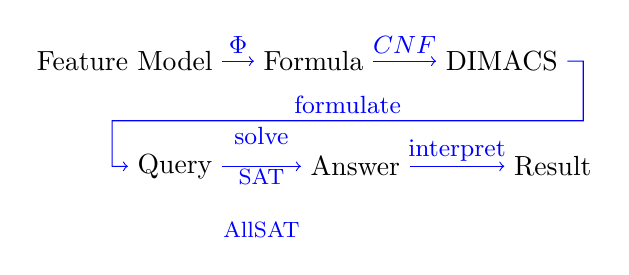
\begin{tikzpicture}
				\tikzset{block/.style={align=center,minimum height=5mm}}
				\node [block] (fm) {Feature Model};
				\node [block, right =4mm of fm] (formula) {Formula};
				\node [block, right =8mm of formula] (cnf) {DIMACS};
				\node [block, below right =8mm and -12mm of fm] (query) {Query};
				\node [block, right =10mm of query] (answer) {Answer};
				\node [block, right =12mm of answer] (result) {Result};
				\node [coordinate, below right =5mm and 2mm of cnf] (right) {};
				\node [coordinate, above left =3mm and 2mm of query] (left) {};
				\path[draw,->,color=blue] (fm) edge node[yshift=2mm] {\small $\Phi$} (formula)
							(formula) edge node[yshift=2mm] {\small $CNF$} (cnf)
							(cnf.east) -| (right) -- node[yshift=2mm] {\small formulate} (left) |- (query)
							(query) edge node[yshift=-2mm,align=center,font={\footnotesize}] {{\small solve}\\[1.5ex]SAT\\\ssat{}\\AllSAT} (answer)
							(answer) edge node [yshift=2mm]{\small interpret} (result);
			\end{tikzpicture}
		}
		\mynote{}{
			for brevity, we assume that $\phi = CNF(\Phi(FM))$ for a given feature model $FM$
		}
	\end{mycolumns}
\end{frame}

\subsection{Consistency, Cardinality, and Enumeration Queries}

\subsubsection{Feature Model}

\begin{frame}{\myframetitle}
	\begin{mycolumns}[t]
		\emph{Consistency of Feature Models (SAT)}
		\mydefinition{Void/Consistent Feature Model}{
			\begin{itemize}
				\item are there grave modeling errors?
				\item is it possible to configure any product at all?
			\end{itemize}
			\centering
			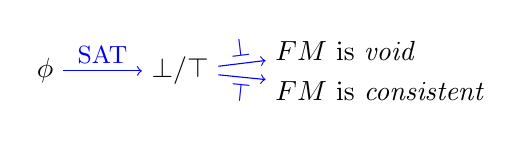
\begin{tikzpicture}
				\tikzset{block/.style={align=center,minimum height=5mm}}
				\node [block] (query) {$\phi$};
				\node [block, right =10mm of query] (answer) {$\bot/\top$};
				\node [block, above right =-3mm and 6mm of answer] (void) {$FM$ is \emph{void}};
				\node [block, below right =-3mm and 6mm of answer] (notvoid) {$FM$ is \emph{consistent}};
				\path[draw,->,color=blue] (query) edge node[yshift=2mm] {\small SAT} (answer)
							(answer) edge node [yshift=2mm,sloped]{\small $\bot$} (void)
							(answer) edge node [yshift=-2mm,sloped]{\small $\top$} (notvoid);
			\end{tikzpicture}
		}
		\mynextcolumn
		\emph{Cardinality of Feature Models (\ssat{})}
		\mydefinition{How Many Products Are There?}{
			\centering
			\begin{tikzpicture}
				\tikzset{block/.style={align=center,minimum height=5mm}}
				\node [block] (query) {$\phi$};
				\node [block, right =10mm of query] (answer) {$\abs{C}$};
				\path[draw,->,color=blue] (query) edge node[yshift=2mm] {\small \ssat{}} (answer);
			\end{tikzpicture}
		}
		\mydefinition{Variability Factor: Share of Products?}{
			\centering
			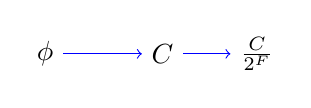
\begin{tikzpicture}
				\tikzset{block/.style={align=center,minimum height=5mm}}
				\node [block] (query) {$\phi$};
				\node [block, right =10mm of query] (answer) {$\abs{C}$};
				\node [block, right =6mm of answer] (num) {$\frac{\abs{C}}{2^{\abs{F}}}$};
				\path[draw,->,color=blue] (query) edge node[yshift=2mm] {\small \ssat{}} (answer)
							(answer) edge node [yshift=2mm,sloped]{} (num);
			\end{tikzpicture}
		}
	\end{mycolumns}
	\begin{mycolumns}[t]
		\myexampletight{}{
			\leftandright{
				\centering
				{\small\featureDiagram{Root,concrete[X,concrete,alternative][Y,concrete]}\\$\pnot (X \por Y)$}

				void
			}{
				\centering
				{\small\featureDiagram{Root,concrete[X,concrete,alternative][Y,concrete]}\\$X \por Y$}

				consistent
			}
		}
		\mynextcolumn
		\myexampletight{}{
			\leftandright{
				\centering
				{\small\featureDiagram{Root,concrete[X,concrete,alternative][Y,concrete]}\\$\pnot (X \por Y)$}

				$0$ products, VF $0$
			}{
				\centering
				{\small\featureDiagram{Root,concrete[X,concrete,alternative][Y,concrete]}\\$X \por Y$}

				$2$ products, VF $\frac{2}{8}$
			}
		}
	\end{mycolumns}
\end{frame}

\begin{frame}{\myframetitle}
	\begin{mycolumns}[t]
		\emph{Feasibility of SAT-Based Analyses}

		\mynote{Is Sat-Based Analysis ``Easy''?}{
			\begin{itemize}
				\item provocative claim: \mycite{SAT-based analysis of feature models is easy} \mysource{\href{https://dl.acm.org/doi/10.5555/1753235.1753267}{Mendonca~et~al.~2009}}
				\item easy $=$ performs much better than expected (although NP-complete)
				\item easy $=$ fast?
				\begin{itemize}
					\item what about formulating the query?\\
						(e.g., CNF transformation)
					\item what about many queries?\\
						(e.g., what we discuss next)
				\end{itemize}
			\end{itemize}
		}
	\mynextcolumn
		\emph{Feasibility of \ssat{}-Based Analyses}
	
		\myexampletight{Time to Count Products of Linux}{
			\includegraphics[width=\linewidth,page=4]{linux-plots}
		}
	\end{mycolumns}
\end{frame}


\begin{frame}{\myframetitle}
	\begin{mycolumns}
		\emph{Enumeration of Feature Models (AllSAT)}
		\mydefinition{Which Products Are There?}{
			\begin{itemize}
				\item \emph{P2(b)}: How to get all products?
			\end{itemize}
			\centering
			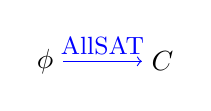
\begin{tikzpicture}
				\tikzset{block/.style={align=center,minimum height=5mm}}
				\node [block] (query) {$\phi$};
				\node [block, right =10mm of query] (answer) {$C$};
				\path[draw,->,color=blue] (query) edge node[yshift=2mm] {\small AllSAT} (answer);
			\end{tikzpicture}
		}
		\mynote{}{
			AllSAT does not scale to realistic feature models!\\
			50 features, configurations \`a 1 Byte $\approx$ 1 Petabyte
		}
		\myexampletight{}{
			\leftandright{
				\centering
				{\small\featureDiagram{Root,concrete[X,concrete,alternative][Y,concrete]}\\$\pnot (X \por Y)$}

				$\varnothing$
			}{
				\centering
				{\small\featureDiagram{Root,concrete[X,concrete,alternative][Y,concrete]}\\$X \por Y$}

				$\{\{Root, X\},\{Root, Y\}\}$
			}
		}
	\mynextcolumn
		\centering
		\sffamily
		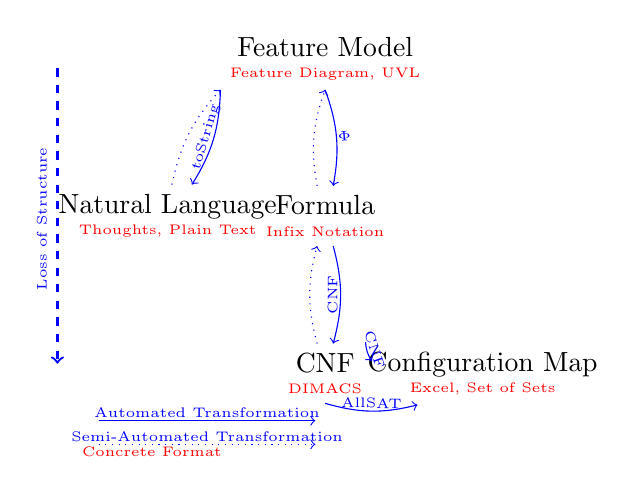
\begin{tikzpicture}
			\tikzstyle{every edge}=[font=\tiny,draw,color=blue]

			\node (topleft) at (-1.4,0) {};
			\node (bottomleft) at (-1.4,-4) {};
			
			\node (fd) at (2,0) [align=center] {Feature Model\\[-1ex]{\tiny\color{red}Feature Diagram, UVL}};
			\node (nat) at (0,-2) [align=center] {Natural Language\\[-1ex]{\tiny\color{red}Thoughts, Plain Text}};
			\node (phi) at (2,-2) [align=center] {Formula\\[-1ex]{\tiny\color{red}Infix Notation}};
			\node (cfg) at (4,-4) [align=center] {Configuration Map\\[-1ex]{\tiny\color{red}Excel, Set of Sets}};
			\node (cnf) at (2,-4) [align=center] {CNF\\[-1ex]{\tiny\color{red}DIMACS}};

			\path [dashed, thick, ->] (topleft) edge node[left, rotate=90, yshift=2mm, xshift=10mm] {Loss of Structure} (bottomleft);
		
			\path [->] (fd.south west) edge[bend left=15] node[sloped,yshift=1mm] {toString} (nat);
			\path [dotted, ->] (nat) edge[bend left=15] node[sloped,yshift=1mm] {} (fd.south west);
			
			\path [->] (fd.south) edge[bend left=15] node[sloped,yshift=1mm,rotate=90] {$\Phi$} (phi);
			\path [dotted, ->] (phi) edge[bend left=15] node[sloped,yshift=2mm,rotate=270] {} (fd.south);

			\path [->] (phi) edge[bend left=15] node[sloped,yshift=1mm] {CNF} (cnf);
			\path [dotted, ->] (cnf) edge[bend left=15] node[sloped,yshift=2mm,rotate=270] {} (phi);
		
			\path [->] (cfg) edge[bend right=15] node[sloped,yshift=1mm] {CNF} (cnf);
			\path [->] (cnf.south) edge[bend right=15] node[sloped,yshift=1mm] {AllSAT} (cfg);

			\node (trans) at (-1,-4.6) {};
			\node (trans2) at (2,-4.6) {};
			\node (trans3) at (-1,-4.9) {};
			\node (trans4) at (2,-4.9) {};
			\path [->] (trans) edge node[yshift=1mm] {Automated Transformation} (trans2);
			\path [dotted, ->] (trans3) edge[yshift=5mm] node[yshift=1mm] {Semi-Automated Transformation} (trans4);
		
			\node (bottomleft2) at (-0.2,-5) {\tiny\color{red}Concrete Format};
		\end{tikzpicture}
	\end{mycolumns}
\end{frame}

\subsubsection{Features}

\begin{frame}{\myframetitle}
	\begin{mycolumns}[t]
		\emph{Consistency of Features (SAT)}
		\mydefinition{Core/Dead Feature}{
			\begin{itemize}
				\item can a feature $F$ be (de-)selected at all?
			\end{itemize}
			\centering
			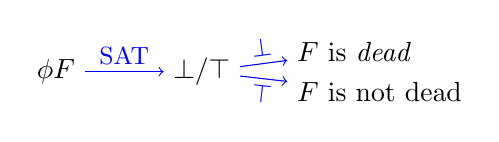
\begin{tikzpicture}
				\tikzset{block/.style={align=center,minimum height=5mm}}
				\node [block] (query) {$\phi \pand F$};
				\node [block, right =10mm of query] (answer) {$\bot/\top$};
				\node [block, above right =-3mm and 6mm of answer] (void) {$F$ is \emph{dead}};
				\node [block, below right =-3mm and 6mm of answer] (notvoid) {$F$ is not dead};
				\path[draw,->,color=blue] (query) edge node[yshift=2mm] {\small SAT} (answer)
							(answer) edge node [yshift=2mm,sloped]{\small $\bot$} (void)
							(answer) edge node [yshift=-2mm,sloped]{\small $\top$} (notvoid);
			\end{tikzpicture}
			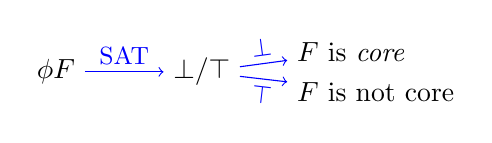
\begin{tikzpicture}
				\tikzset{block/.style={align=center,minimum height=5mm}}
				\node [block] (query) {$\phi \pand \pnot F$};
				\node [block, right =10mm of query] (answer) {$\bot/\top$};
				\node [block, above right =-3mm and 6mm of answer] (void) {$F$ is \emph{core}};
				\node [block, below right =-3mm and 6mm of answer] (notvoid) {$F$ is not core};
				\path[draw,->,color=blue] (query) edge node[yshift=2mm] {\small SAT} (answer)
							(answer) edge node [yshift=2mm,sloped]{\small $\bot$} (void)
							(answer) edge node [yshift=-2mm,sloped]{\small $\top$} (notvoid);
			\end{tikzpicture}
		}
		\mynextcolumn
		\emph{Cardinality of Features (\ssat{})}
		\mydefinition{How Many Products Include Feature $F$?}{
			\centering
			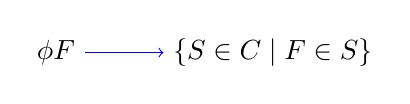
\begin{tikzpicture}
				\tikzset{block/.style={align=center,minimum height=5mm}}
				\node [block] (query) {$\phi \pand F$};
				\node [block, right =10mm of query] (answer) {$\abs{\{S \in C \mid F \in S\}}$};
				\path[draw,->,color=blue] (query) edge node[yshift=2mm] {\small \ssat{}} (answer);
			\end{tikzpicture}
		}
		\mydefinition{Commonality: How Dead is This Feature?}{
			\centering
			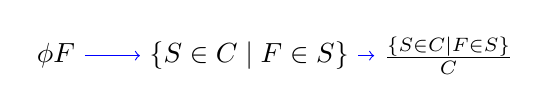
\begin{tikzpicture}
				\tikzset{block/.style={align=center,minimum height=5mm}}
				\node [block] (query) {$\phi \pand F$};
				\node [block, right =7mm of query] (answer) {$\abs{\{S \in C \mid F \in S\}}$};
				\node [block, right =2mm of answer] (num) {$\frac{\abs{\{S \in C \mid F \in S\}}}{\abs{C}}$};
				\path[draw,->,color=blue] (query) edge node[yshift=2mm] {\small \ssat{}} (answer)
							(answer) edge node [yshift=2mm,sloped]{} (num);
			\end{tikzpicture}
		}
	\end{mycolumns}
	\begin{mycolumns}[t]
		\myexampletight{}{
			\centering
			{\small\featureDiagram{Root,concrete[X,concrete,alternative][Y,concrete]}\\$\pnot X$}

			$X$ is dead, $Root$ and $Y$ are core
		}
		\mynextcolumn
		\myexampletight{}{
			\centering
			{\small\featureDiagram{Root,concrete[X,concrete,alternative][Y,concrete]}\\$\pnot X$}

			$X$: 0 products, $Root$ and $Y$: 1 products
		}
	\end{mycolumns}
\end{frame}

\subsubsection{Partial Configurations}

\begin{frame}{\myframetitle}
	\begin{mycolumns}[t]
		\emph{Consistency of Partial Configurations (SAT)}
		\mydefinition{Valid Partial Configuration}{
			\begin{itemize}
				\item does a partial configuration $C = ({\color{green}S}, {\color{red}D})$ contain a mistake?
			\end{itemize}
			\centering
			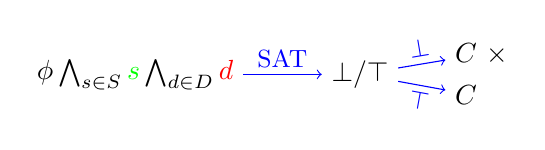
\begin{tikzpicture}
				\tikzset{block/.style={align=center,minimum height=5mm}}
				\node [block] (query) {$\phi \pand \bigwedge_{s \in S} {\color{green}s} \pand \bigwedge_{d \in D} {\color{red}\pnot d}$};
				\node [block, right =10mm of query] (answer) {$\bot/\top$};
				\node [block, above right =-3mm and 6mm of answer] (void) {$C$ $\times$};
				\node [block, below right =-3mm and 6mm of answer] (notvoid) {$C$ \checkmark};
				\path[draw,->,color=blue] (query) edge node[yshift=2mm] {\small SAT} (answer)
							(answer) edge node [yshift=2mm,sloped]{\small $\bot$} (void)
							(answer) edge node [yshift=-2mm,sloped]{\small $\top$} (notvoid);
			\end{tikzpicture}
		}
		\mynextcolumn
		\emph{Cardinality of Partial Configurations (\ssat{})}
		\mydefinition{How Many Products Are Still Configurable for $C$?}{
			\centering
			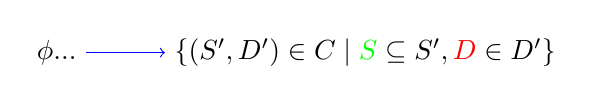
\begin{tikzpicture}
				\tikzset{block/.style={align=center,minimum height=5mm}}
				\node [block] (query) {$\phi \pand ...$};
				\node [block, right =10mm of query] (answer) {$\abs{\{(S', D') \in C \mid {\color{green}S} \subseteq S', {\color{red}D} \in D'\}}$};
				\path[draw,->,color=blue] (query) edge node[yshift=2mm] {\small \ssat{}} (answer);
			\end{tikzpicture}
		}
	\end{mycolumns}
	\begin{mycolumns}[t]
		\myexampletight{}{
			\centering
			{\small\featureDiagram{Root,concrete[X,concrete,optional][Y,concrete,optional]}\\$X \pimplies Y$}

			\cfg{Root}{X} \checkmark
		}
		\mynextcolumn
		\myexampletight{}{
			\centering
			{\small\featureDiagram{Root,concrete[X,concrete,optional][Y,concrete,optional]}\\$X \pimplies Y$}

			\cfg{Root}{X}: 2 products
		}
	\end{mycolumns}
\end{frame}

\subsection{Automated Analyses in FeatureIDE}

\subsubsection*{Feature-Model Editor}

\begin{frame}{\myframetitle}
	\begin{mycolumns}[widths={60,40}]
		\myexampletight{}{
			\pic[width=\textwidth]{featureide-feature-model-editor-waffle}
		}
	\mynextcolumn
		\myexampletight{}{
			\pic[width=\textwidth]{featureide-feature-model-statistics}
		}
	\end{mycolumns}
\end{frame}

\subsubsection*{Configuration Editor}

\begin{frame}{\myframetitle}
	\begin{mycolumns}[widths={60,40}]
		\myexampletight{}{
			\centering
			\pic[width=.27\textwidth]{featureide-configuration-editor-step1}
			$\Rightarrow$
			\pic[width=.63\textwidth]{featureide-configuration-editor-step2}
		}
	\mynextcolumn
		\mynote{Decision Propagation}{
			\begin{itemize}
				\item after each decision (i.e., click) \ldots
				\begin{itemize}
					\item \ldots{} select features that are now \emph{conditionally core}
					\item \ldots{} deselect features that are now \emph{conditionally dead}
				\end{itemize}
				\item this way it is impossible to configure an invalid product
				\item explanations for all propagated decisions
			\end{itemize}
		}
	\end{mycolumns}
\end{frame}

\begin{frame}{Automated Analysis of Feature Models}
	\begin{mycolumns}
		\mydefinition{The Road So Far \ldots}{
			\centering
			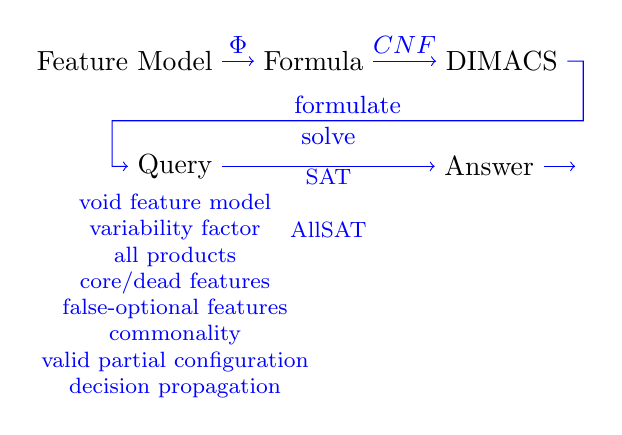
\begin{tikzpicture}
				\tikzset{block/.style={align=center,minimum height=5mm}}
				\node [block] (fm) {Feature Model};
				\node [block, right =4mm of fm] (formula) {Formula};
				\node [block, right =8mm of formula] (cnf) {DIMACS};
				\node [block, below right =8mm and -12mm of fm] (query) {Query};
				\node [block, below =-.5mm of query,align=center,color=blue,font={\footnotesize}] (query2) {void feature model\\variability factor\\all products\\core/dead features\\false-optional features\\commonality\\valid partial configuration\\decision propagation};
				\node [block, right =27mm of query] (answer) {Answer};
				\node [block, right =4mm of answer] (result) {};
				\node [coordinate, below right =5mm and 2mm of cnf] (right) {};
				\node [coordinate, above left =3mm and 2mm of query] (left) {};
				\path[draw,->,color=blue] (fm) edge node[yshift=2mm] {\small $\Phi$} (formula)
							(formula) edge node[yshift=2mm,align=center] {\small $CNF$} (cnf)
							(cnf.east) -| (right) -- node[yshift=2mm] {\small formulate} (left) |- (query)
							(query) edge node[yshift=-2mm,align=center,font={\footnotesize}] {{\small solve}\\[1.5ex]SAT\\\ssat{}\\AllSAT} (answer)
							(answer) edge (result);
			\end{tikzpicture}
		}
	\mynextcolumn
		\mydefinition{\ldots and Beyond}{
			\centering
			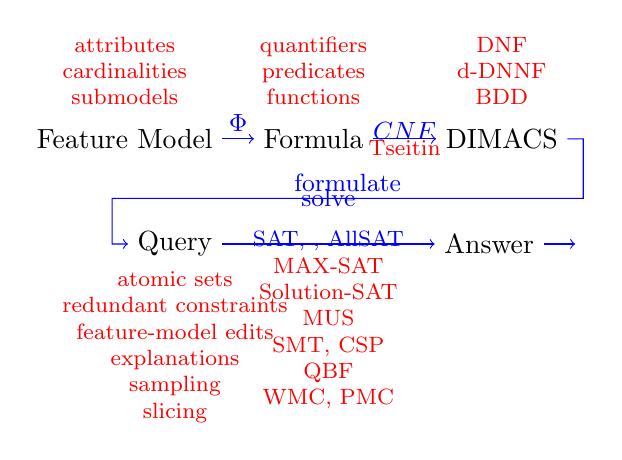
\begin{tikzpicture}
				\tikzset{block/.style={align=center,minimum height=5mm}}
				\node [block,align=center,color=red,font={\footnotesize}] (fm2) {attributes\\cardinalities\\submodels};
				\node [block, below =.5mm of fm2] (fm) {Feature Model};
				\node [block, right =4mm of fm] (formula) {Formula};
				\node [block, above =.5mm of formula,align=center,color=red,font={\footnotesize}] (formula2) {quantifiers\\predicates\\functions};
				\node [block, right =8mm of formula] (cnf) {DIMACS};
				\node [block, above =.5mm of cnf,align=center,color=red,font={\footnotesize}] (cnf2) {DNF\\d-DNNF\\BDD};
				\node [block, below right =8mm and -12mm of fm] (query) {Query};
				\node [block, below =-.5mm of query,align=center,color=red,font={\footnotesize}] (query2) {atomic sets\\redundant constraints\\feature-model edits\\explanations\\sampling\\slicing};
				\node [block, right =27mm of query] (answer) {Answer};
				\node [block, right =4mm of answer] (result) {};
				\node [coordinate, below right =5mm and 2mm of cnf] (right) {};
				\node [coordinate, above left =3mm and 2mm of query] (left) {};
				\path[draw,->,color=blue] (fm) edge node[yshift=2mm] {\small $\Phi$} (formula)
							(formula) edge node[yshift=0mm,align=center] {\small $CNF$\\{\footnotesize\color{red}Tseitin}} (cnf)
							(cnf.east) -| (right) -- node[yshift=2mm] {\small formulate} (left) |- (query)
							(query) edge node[yshift=-7mm,align=center,font={\footnotesize}] {{\small solve}\\[1.5ex]SAT, \ssat{}, AllSAT\\{\color{red}MAX-SAT}\\{\color{red}Solution-SAT}\\{\color{red}MUS}\\{\color{red}SMT, CSP}\\{\color{red}QBF}\\{\color{red}WMC, PMC}} (answer)
							(answer) edge (result);
			\end{tikzpicture}
			\vspace*{-4ex}
			\begin{itemize}
				\item develop new analyses
				\item improve efficiency of existing analyses
				\item investigate correctness and compositionality
			\end{itemize}
		}
	\end{mycolumns}
\end{frame}
\lessonslearned{
	\item with solvers, we can build reliable configurators for product lines
	\item SAT-based analyses: void feature model, core/dead features, decision propagation
	\item \ssat{}-based analyses: variability factor, feature commonality
}{ % TODO unify literature pointer (see Lecture 1-3)
	\item \fospl\mysection{10.1}\mypages{244--254}\\--- introduction to feature-model analysis
	\item David Benavides et al. (2010): \href{https://doi.org/10.1016/j.is.2010.01.001}{Automated Analysis of Feature Models 20 Years Later: A Literature Review}\\--- old but extensive literature survey
	\item Chico Sundermann et al. (2021): \href{https://doi.org/10.1145/3442391.3442404}{Applications of \#SAT Solvers on Feature Models}\\--- experiments on the scalability of \ssat{} solvers % TODO replace by EMSE paper?
	% TODO we could add the paper about web configurators here
}{
	\begin{center}
		\featureDiagramABCDE
	\end{center}

	think of a constraint that would make exactly one feature dead
%	How can you \ldots
%	\begin{enumerate}
%		\item make this feature model void
%		\item make exactly one feature dead
%	\end{enumerate}
%	\ldots{} by adding one constraint, respectively?
%
%	Name a partial configuration for which only two products exist.
}

\faq{
	\item What is feature modeling? When is it needed?
	\item How can we specify valid combinations of features?
	\item What is a complete, partial, valid, invalid configuration?
	\item What are (dis-)advantages of natural language, configuration map, and feature models?
	\item What is the graphical syntax and semantics of feature models?
	\item Give an example feature model!
}{
	\item What representations of feature models are available? Are they equivalent?
	\item How to represent feature models textually?
	\item What is UVL (used for)?
	\item How to identify whether a configuration is valid?
	\item How to translate feature model into a propositional formula?
	\item What are DIMACS and KConfig (used for)?
	\item Would you recommend Excel for feature model? Why (not)?
}{
	\item Why can configuration become challenging?
	\item How can we identify problems with feature models and configurations?
	\item How can feature models by analyzed? What analyses are available?
	\item What solvers can be used to analyze feature models?
	\item What is the difference between SAT, \ssat, and ALLSAT?
	\item Why are solvers useful when creating configurations?
}

\mode<beamer>{
	\begin{frame}{\inserttitle}
		\lectureseriesoverview
	\end{frame}

	\contentoverview
}


% TODO L05 CONDITIONAL COMPILATION

\ifuniversity{recording}{\date{April 23, 2023}\setpicture[75]{may21-north2}\setcopyright{}}
\ifuniversity{ulm}{\date{May 11, 2023}\setpicture[75]{may21-north2}}
\ifuniversity{magdeburg}{\setpicture[300]{magdeburg-river}\setcopyright{}}

\author{Thomas Thüm, Elias Kuiter, Timo Kehrer}
\lecture{Conditional Compilation}{conditional}

% TODO shall we use conditional compilation with build systems (preprocessors) instead? would require numerous changes in this lecture
\section{Features with Build Systems}
\subsection{How to Implement Features?}
\begin{frame}{\myframetitle}
	\begin{mycolumns}
		\begin{exampletight}{Given a feature model for graphs \ldots}
			\centering\featureDiagramGraphs
			%\featureDiagramLegend
		\end{exampletight}
		\begin{example}{\ldots\ we can derive a valid configuration}
			\small
			\begin{mycolumns}[columns=3,animation=none]
				$\{G\}$\\
				$\{G,C\}$\\
				$\{G,D\}$\\
				$\{G,C,D\}$\\
			\mynextcolumn
				$\{G,W\}$\\
				$\{G,C,W\}$\\
				$\{G,D,W\}$\\
				$\{G,C,D,W\}$\\
			\mynextcolumn
				$\{G,W,S\}$\\
				$\{G,C,W,S\}$\\
				$\{G,D,W,S\}$\\
				$\{G,C,D,W,S\}$\\
			\end{mycolumns}
		\end{example}
	\mynextcolumn
		\vspace{-10mm}\pause
		\begin{exampletight}{How to Generate Products Automatically?}
			\centering\foreach \page in {2,12,4,14,6,16,8,18,10,20,42,44}{\pic[width=.23\linewidth,page=\page]{graphs} }
		\end{exampletight}
		\begin{note}{Goals}
			\begin{itemize}
				\item descriptive specification of a product (i.e., a configuration, a selection of features)
				\item automated generation of a product with compile-time variability
			\end{itemize}
			Focus of the next three lectures \ldots
		\end{note}
	\end{mycolumns}
\end{frame}

\subsection{Problems of Ad-Hoc Approaches for Variability}

\subsubsection{Features with Runtime Variability?}
\againframe<2>{GraphWithGlobalVariables}

\begin{frame}{\myframetitle}
	\begin{mycolumns}[b,widths={36}]
		\picDark[width=\linewidth]{preferences-eclipse}

		\begin{definition}{How to? -- Preference Dialog}
			\begin{itemize}
				\item implement runtime variability
				\item compile the program
				\item run the program
				\item \emph{manually adjust preferences based on configuration}
			\end{itemize}
		\end{definition}
	\mynextcolumn
		\begin{mycolumns}[widths={41},animation=none]
			\pic[width=\linewidth]{runtime-parameters-win10-cmd-dir}
		\mynextcolumn
			\picDark[width=\linewidth]{configfile-eclipse-ini}
		\end{mycolumns}

		\begin{definition}{How to? -- Command-Line Options / Configuration Files}
			\begin{itemize}
				\item implement runtime variability
				\item compile the program
				\item \emph{automatically generate command-line options / configuration files based on configuration}
				\item run the program
			\end{itemize}
		\end{definition}
	\end{mycolumns}
\end{frame}

\begin{frame}[fragile]{\myframetitle}
	\begin{mycolumns}[widths={48}]
\begin{codetight}[basicstyle=\small]{}
public class Config {
	~public final static boolean COLORED = true;~
	@public final static boolean WEIGHTED = false;@
}
\end{codetight}
		\begin{definition}{How to? -- Immutable Global Variables}
			\begin{itemize}
				\item implement runtime variability
				\item automatically generate class with global variables based on configuration
				\item compile and run the program
			\end{itemize}
		\end{definition}
	\mynextcolumn
		\begin{note}{What is missing?}
			\begin{itemize}
				\item automated generation:\\\hfill for preference dialogs
				\item no compile-time variability / same large binary:\\\hfill for all except immutable global variables
				\item very limited compile-time variability:\\\hfill for immutable global variables
			\end{itemize}
		\end{note}
	\end{mycolumns}
\end{frame}

\subsubsection{Features with Clone-and-Own?}
\begin{frame}{\myframetitle}
	\begin{mycolumns}[widths={30},animation=none]
		\centering~

		\picDark[scale=0.2]{alice}
		\pic[scale=0.26,page=2]{graphs}

		\picDark[scale=0.2]{bob}
		\pic[scale=0.26,page=12]{graphs}

		\picDark[scale=0.2]{eve}
		\pic[scale=0.26,page=16]{graphs}
	\mynextcolumn
		\begin{definition}{How to?}
			\begin{itemize}
				\item implement separate project for each product\\(i.e., branch with version control)
				\item download project / checkout branch based on configuration
				\item run build script, if existent
				\item compile and run the program
			\end{itemize}
		\end{definition}
		\pause
		\begin{note}{What is missing?}
			\begin{itemize}
				\item compile-time variability only for implemented products
				\item no automated generation:\\\hfill for clone-and-own (with version control systems)
				\item automated generation based on build script and extra files:\\\hfill for clone-and-own with build systems
				\item no free feature selection (i.e., configuration)
			\end{itemize}
		\end{note}
	\end{mycolumns}
\end{frame}

\subsection{Recap: Clone-and-Own with Build Systems}
\begin{frame}{\myframetitle\  \mytitlesource{\href{https://dl.acm.org/doi/10.1145/3461002.3473950}{Kuiter~et~al.~2021}}}
	\begin{mycolumns}[columns=2,widths={76},animation=none]
		\begin{mycolumns}[widths={50},animation=none] % TODO widths needed due to bug #56 in slide template
			\begin{example}{Case Study: Anesthesia Device}
				\begin{itemize}
					\item C application
					\item targets embedded devices (ESP32)
					\item configurations are hard-coded as build scripts
				\end{itemize}
			\end{example}
		\mynextcolumn
			\uncover<4->{
				\begin{exampletight}{{\color{red}Production Device}: OLED, Clock}
					\centering\pic[height=25mm]{pignap-cfg-production-oled}
				\end{exampletight}
			}
		\end{mycolumns}
		\begin{mycolumns}[widths={50},animation=none] % TODO widths needed due to bug #56 in slide template
			\uncover<2->{
				\begin{exampletight}{{\color{green}Prototype}: OLED Display}
					\centering\pic[height=25mm]{pignap-cfg-prototype-oled}
				\end{exampletight}
			}
		\mynextcolumn
			\uncover<3->{
				\begin{exampletight}{{\color{blue}Prototype}: LCD, Real-Time Clock}
					\centering\pic[height=25mm]{pignap-cfg-prototype-lcd-rtc}
				\end{exampletight}
			}
		\end{mycolumns}
	\mynextcolumn
		\only<1|handout:0>{\pic[width=\linewidth,page=1]{pignap-variants}}%
		\only<2|handout:0>{\pic[width=\linewidth,page=2]{pignap-variants}}%
		\only<3|handout:0>{\pic[width=\linewidth,page=3]{pignap-variants}}%
		\only<4->{\pic[width=\linewidth,page=4]{pignap-variants}}
	\end{mycolumns}
\end{frame}

\subsection{Introducing Features to Build Systems}
\begin{frame}{\myframetitle\  \mytitlesource{\href{https://dl.acm.org/doi/10.1145/3461002.3473950}{Kuiter~et~al.~2021}}}
	\begin{mycolumns}[widths={60}]
		\begin{definition}{How to Implement Features with Build Systems?}
			\begin{itemize}
				\item step 1: model variability in a feature model
				\item step 2: in build scripts, in- and exclude files based on feature selection
				\item step 3: pass a feature selection at build time
			\end{itemize}
			$\Rightarrow$ one build script per group of related features
		\end{definition}
		\begin{center}
			\featureDiagram{Anesthesia Device,abstract
			[Monitoring,abstract,mandatory
				[Display,abstract,or[LCD,concrete,alternative][OLED,concrete]]
				[Wi-Fi,abstract
					[HTTP Server,concrete,mandatory]]]
			[History,optional,concrete]
			[Libraries,abstract,mandatory
				[Storage,abstract,optional[NVS,concrete,alternative][FRAM,concrete]]
				[RTC,concrete,optional[Battery,concrete,mandatory]]]}

			$History \pimplies Storage \pand RTC$
		\end{center}
	\mynextcolumn
		\centering\pic[height=\textheightwithtitle]{pignap-features}
	\end{mycolumns}
\end{frame}

\subsection{The Linux Kernel}

\xkcdframe{619} % linux features 20s

\subsubsection*{KConfig for Feature Modeling}

\begin{frame}[fragile]{\myframetitle}
	\begin{mycolumns}
		\begin{kconfigtight}[basicstyle=\small]{Part of the x86 Architecture \mysource{\href{https://github.com/torvalds/linux/blob/0326074/arch/x86/Kconfig}{linux/arch/x86/Kconfig}}}
config 64BIT
	bool "64-bit kernel" if "$(ARCH)" = "x86"
	default "$(ARCH)" != "i386"
	help
		Say yes to build a 64-bit kernel (x86_64)
		Say no to build a 32-bit kernel (i386)

config X86_32
	def_bool y
	depends on !64BIT
	# Options that are inherently 32-bit kernel only:
	select GENERIC_VDSO_32
	select ARCH_SPLIT_ARG64

config X86_64
	def_bool y
	depends on 64BIT
	# Options that are inherently 64-bit kernel only:
	select ARCH_HAS_GIGANTIC_PAGE
	select ARCH_SUPPORTS_INT128 if CC_HAS_INT128
\end{kconfigtight}
	\mynextcolumn
		\begin{definition}{KConfig Language\mysource{\href{https://www.kernel.org/doc/html/latest/kbuild/kconfig-language.html}{kernel.org}}}
			\begin{itemize}
				\item configuration language used in embedded/OS development (e.g., Linux, Zephyr, ESP32)
				\item similar to UVL, but has many quirks (e.g., tristate features, \texttt{select})
				\item transformation into formula or feature model possible, but not trivial \mysource{\href{https://dl.acm.org/doi/abs/10.1145/3468264.3468578}{Oh~et~al.~2021}}
			\end{itemize}
		\end{definition}
		\hspace*{-0.07253886\linewidth}%=2*0.035/(1-0.035)
		\linuxbddlink{\pic[width=1.3\linewidth,trim=220 510 60 180,clip]{2020/2020-SPLC-Thuem}}
	\end{mycolumns}
\end{frame}

\subsubsection*{MenuConfig for Configuration}

\begin{frame}{\myframetitle}
	\begin{mycolumns}[widths={60,40}]
		\begin{exampletight}{}
			\pic[width=\textwidth]{linux-menuconfig} % sudo apt install make flex bison libncurses5-dev && make menuconfig
		\end{exampletight}
	\mynextcolumn
		\begin{note}{make menuconfig}
			\begin{itemize}
				\item configures KConfig models
				\item generates a \texttt{.config} file
				\item widely used to configure Linux
				\item still: it is possible to create invalid configurations and products % TODO does not fit into the storyline anymore. remove?
			\end{itemize}
		\end{note}
	\end{mycolumns}
\end{frame}

\subsubsection*{KBuild as Build System}

\begin{frame}[fragile]{\myframetitle}
	\begin{mycolumns}
		\begin{kconfigtight}[basicstyle=\footnotesize]{Feature Model with KConfig\mysource{\href{https://github.com/torvalds/linux/blob/0326074/arch/x86/Kconfig}{linux/arch/x86/Kconfig}}}
config X86_32 ...
config X86_64 ...

config IA32_EMULATION
	bool "IA32 Emulation"
	depends on X86_64
	help Include code to run legacy 32-bit programs under a 64-bit kernel. You should likely enable this, unless you're 100% sure that you don't have any 32-bit programs left.
\end{kconfigtight}
		\begin{definition}{KBuild\mysource{\href{https://www.kernel.org/doc/html/latest/kbuild/makefiles.html}{kernel.org}}}
			\begin{itemize}
				\item a style for writing Makefiles in Linux
				\item defines goals with Make variables
				\begin{itemize}
					\item \texttt{obj-y}: static linkage (= include feature)
					\item \texttt{obj-m}: dynamic linkage (= as module)
					\item \texttt{obj-}: no linkage (= exclude feature)
				\end{itemize}
				\item full power of Make $\Rightarrow$ hard to comprehend
			\end{itemize}
		\end{definition}
	\mynextcolumn
		\begin{kbuildtight}[basicstyle=\small]{Feature Mapping with KBuild \mysource{\href{https://github.com/torvalds/linux/blob/0326074/arch/x86/Kbuild}{linux/arch/x86/Kbuild}}}
# link these subdirectories statically:
obj-y += entry/ # entry routines
obj-y += realmode/ # 16-bit support
obj-y += kernel/ # x86 kernel
obj-y += mm/ # memory management

# link these depending on a configuration option:
obj-~$(CONFIG_IA32_EMULATION)~ += ia32/
obj-~$(CONFIG_XEN)~ += xen/ # paravirtualization

# the KConfig feature model can even be overridden:
obj-~$(subst m,y,$(CONFIG_HYPERV))~ += hyperv/
		\end{kbuildtight}

		\begin{kbuildtight}[basicstyle=\small]{Recurse into Subsystems\mysource{\href{https://github.com/torvalds/linux/blob/0326074/arch/x86/ia32/Makefile}{linux/arch/x86/ia32/Makefile}}}
# ia32 kernel emulation subsystem
obj-~$(CONFIG_IA32_EMULATION)~ := ia32_signal.o
audit-class-~$(CONFIG_AUDIT)~ := audit.o

# IA32_EMULATION and AUDIT required for audit.o:
obj-~$(CONFIG_IA32_EMULATION)~ += ~$(audit-class-y)~
		\end{kbuildtight}
	\end{mycolumns}
\end{frame}

\begin{frame}[fragile]{\myframetitle}
	\begin{mycolumns}
		\begin{example}{Interactive Linux Kernel Configurator}
			\pic[width=\linewidth]{linux-menuconfig-emulation}
		\end{example}

		\begin{kconfigtight}[basicstyle=\footnotesize]{Feature Model and Example Configuration}
			config AUDIT ... # configured as NO
			config IA32_EMULATION ... # configured as YES
			config HYPERV ... # configured as MODULE
			config XEN ... # configured as NO
\end{kconfigtight}
	\mynextcolumn
		\begin{kbuildtight}[basicstyle=\small]{Feature Mapping}
obj-y += entry/ realmode/ kernel/ mm/
obj-~$(CONFIG_IA32_EMULATION)~ += ia32/
obj-~$(CONFIG_XEN)~ += xen/
obj-~$(subst m,y,$(CONFIG_HYPERV))~ += hyperv/
obj-~$(CONFIG_IA32_EMULATION)~ := ia32_signal.o
audit-class-~$(CONFIG_AUDIT)~ := audit.o
obj-~$(CONFIG_IA32_EMULATION)~ += ~$(audit-class-y)~
		\end{kbuildtight}

		\begin{kbuildtight}[basicstyle=\small]{Feature Mapping for Example Configuration}
obj-y += entry/ realmode/ kernel/ mm/
obj-?y? += ia32/
obj- += xen/
obj-?y? += hyperv/
obj-?y? := ia32_signal.o
audit-class- := audit.o
obj-?y? +=
		\end{kbuildtight}

		\begin{note}{}
			\small i.e., \texttt{entry, realmode, kernel, mm, ia32, hyperv, ia32\_signal.o} are compiled
		\end{note}
	\end{mycolumns}
\end{frame}

% TODO add quote? \mycite{As Kbuild relies on a Turing-complete language, complex conditions can be encoded.} \mysource{\fospl\mypage{108}}

\subsection{Discussion of Features with Build Systems}
\begin{frame}{\myframetitle}
	\begin{mycolumns}
		\begin{note}{Advantages}
			\begin{itemize}
				\item compile-time variability\\
					$\Rightarrow$ \emph{fast, small binaries} with smaller attack surface and without disclosing secrets
				\item automated generation of arbitrary products\\
					$\Rightarrow$ \emph{free feature selection}
				\item allows in- and exclusion of individual files or even entire subsystems\\
					$\Rightarrow$ high-level, \emph{modular variability}
			\end{itemize}
		\end{note}
	\mynextcolumn
		\begin{note}{Challenges}
			\begin{itemize}
				\item not easily reconfigurable at run- or load-time
				\item build scripts may become complex, there is no limit to what can be done (e.g., you can run arbitrary shell commands on files)\\
					$\Rightarrow$ \emph{hard to understand and analyze}
				\item no simple in- and exclusion of individual lines or chunks of code\\
				$\Rightarrow$ high-level use \emph{only}!
			\end{itemize}
		\end{note}
	\end{mycolumns}
\end{frame}

\lessonslearned{
	\item ad-hoc variability is lacking
	\item features with build systems allow for automated generation of products and free feature selection
	\item build systems include entire files, not lines or chunks
}{
	\item \fospl\mychapter{5.2.1}\mypages{105--106}\\--- brief introduction to variability in build scripts
	% TODO add literature? van der Storm T (2004).Variability and component composition. In: Proc. Int’l Conf. Software Reuse (ICSR) Lecture notes in computer science, vol 3107. Springer, pp 157–166
	\item \fospl\mychapter{5.2.3}\mypages{107--108}\\--- variability in build scripts of the Linux kernel
	% TODO add literature? Berger T, She S, Czarnecki K, Wa ̨sowski A (2010a) Feature-to-code mapping in two large product lines. In: Proc. Int’l Software Product Line Conference (SPLC). Lecture Notes in Computer Science, vol 6287. Springer, pp 498–499
	% TODO add literature? Dietrich C, Tartler R, Schröder-Preikschat W, Lohmann D (2012b) Understanding Linux feature distribution. In: Proc. AOSD Workshop on Modularity In Systems Software (MISS). ACM Press, pp 15–20
	% TODO add work on KernelHaven
}{
% example replaced, as this is probably better for the actual exercise
%	Choose a build system and sketch how it may be used to implement this SPL (file structure and build script):
%
%	\begin{center}
%		\small\featureDiagramConfigurableDatabase
%	\end{center}
	\begin{enumerate}
		\item How are features implemented with build systems different from clone-and-own with build systems?
		\item What is the respective granularity?
	\end{enumerate}

	\uploadpractice
}

\section{Features with Preprocessors}
\subsection{Granularity of Variability}
\begin{frame}{\myframetitle}
	\begin{mycolumns}
		\todots
	\mynextcolumn
		\todots
	\end{mycolumns}
\end{frame}
% Christian's paper?
% empirical studies?
% essence: file-level variability is not engough

\subsection{What is a Preprocessor?}
\begin{frame}{\myframetitle\mysource{\fospl\mypages{110--111}}}
	\begin{mycolumns}
		\begin{definition}{Preprocessor}
			\begin{itemize}
				\item tool manipulating source code before compilation (i.e., at compile time)
				\item preprocessors are used:
					\begin{itemize}
						\item to inline files\hfill(e.g., header files)
						\item to define and expand macros\\\hfill(cf.\ metaprogramming)
						\item for \textbf{conditional compilation}\\\hfill(e.g., remove debug code for release)
					\end{itemize}
			\end{itemize}
		\end{definition}
	\mynextcolumn
		\begin{note}{Preprocessor}
			\begin{itemize}
				\item the C Preprocessor is used in almost every C/C++ project
				\item preprocessors are typically oblivious to the target language as they operate on text files (e.g., the C Preprocessor can also used for Fortran or Java)
				\item conditional compilation is a very common technique to implement product lines
			\end{itemize}
		\end{note}
	\end{mycolumns}
\end{frame}

% in-place vs outa-place preprocessors
% how to select features? parameters passed to the preprocessor, define in source code

\subsection{CPP -- The C Preprocessor}
\begin{frame}{\myframetitle\ -- In a Nutshell \mytitlesource{\featureide}}
	\leftorright{
		\myexampletight{Example Input to the Preprocessor}{\includegraphics[scale=.3]{preprocessor-c}}
	}{
		\myexampletight{Example Output (Simplified)}{\includegraphics[scale=.15]{preprocessor-c-output}}
		\begin{note}{}
			preprocessors typically do not remove line breaks to not influence of line numbers reported by compilers
		\end{note}
	}
\end{frame}
% TODO example contains "Beautiful" but should be "beautiful"
% TODO keywords: #ifdef #endif #else
% TODO illustrate parameters and the call of the preprocessor

\begin{frame}{\myframetitle\ -- In a Coconutshell}
	\todots
\end{frame}
% TODO explain the most important commands: #if #defined or and not ... #elif
% TODO #include

% TODO #error
% TODO parameters, #define, even combinations

% TODO single characters
% TODO discipliced, undisciplined

\subsection{Preprocessors for Java}
\begin{frame}{Munge -- A Simple Preprocessor for Java \mytitlesource{\featureide}}
	\begin{mycolumns}[widths={55}]
		\myexampletight{Example Input and Output}{\includegraphics[width=\linewidth]{preprocessor-munge}}
	\mynextcolumn
		\myexampletight{Calling the Preprocessor}{
			\centering
			\includegraphics[width=\linewidth]{preprocessor-munge-call}
			
			\includegraphics[width=.7\linewidth]{preprocessor-munge-idea}
		}
	\end{mycolumns}
\end{frame}

\begin{frame}{Antenna -- An In-Place Preprocessor for Java \mytitlesource{\featureide}}
	\begin{mycolumns}[widths={55}]
		\myexampletight{Example Input and Output}{\includegraphics[width=\linewidth]{preprocessor-antenna}}
	\mynextcolumn
		\myexampletight{Calling the Preprocessor}{
			\centering
			\includegraphics[width=\linewidth]{preprocessor-antenna-call}
			
			~
			
			\includegraphics[width=.7\linewidth]{preprocessor-antenna-idea}
		}
	\end{mycolumns}
\end{frame}

\subsection{Preprocessors in FeatureIDE}
\begin{frame}{\myframetitle\mysource{\featureide}}
	\begin{mycolumns}[animation=none,widths={75}]
		\only<1|handout:0>{\pic[width=\linewidth]{featureide-antenna-featuremodel}}%
		\only<2|handout:1>{\pic[width=\linewidth]{featureide-antenna-configuration}}%
		\only<3|handout:0>{\pic[width=\linewidth]{featureide-antenna-warning}}%
		\only<4|handout:0>{\pic[width=\linewidth]{featureide-antenna-contentassist}}%
	\mynextcolumn
%		\begin{definition}{FeatureIDE\mysource{\featureide}}
%			\begin{itemize}
%				\item 
%			\end{itemize}
%		\end{definition}
		\begin{note}{\href{https://www.youtube.com/watch?v=jVe7f32mLCQ}{Demo Video}}
			\begin{itemize}
				\item preprocessing with Antenna on command line
				\item feature modeling
				\item warnings for unreferenced features
				\item content assist proposing feature names
				\item configuration and automated regeneration
				\item (first 2 min relevant here)
			\end{itemize}
		\end{note}
	\end{mycolumns}
\end{frame}
% TODO has FeatureIDE been shown/discussed before? ideally, here only present preprocessor integration

\subsection{Discussion of Preprocessors}
\begin{frame}{\myframetitle\ \mytitlesource{\featureide}}
	\leftorright{
		\myexampletight{A Slightly More Complex Example}{\includegraphics[width=\linewidth]{preprocessor-antenna-elevator}}
	}{
		\todots
	}
\end{frame}
% pros: fine granular, language-independent
% cons: IDE support, easy to create mistakes

\xkcdframe{619} % linux features 20s

\subsection{Preprocessor-Based Product Lines in the Wild}
\begin{frame}{\myframetitle\mysource{\fortyproductlines}}
	\leftorright{
		\begin{exampletight}{Number of Features}
			\centering\pic[width=.8\linewidth,page=1]{fortyproductlines}\\Lines of Code
		\end{exampletight}
	}{
		\begin{exampletight}{Percentage of Variable Code}
			\centering\pic[width=.8\linewidth,page=2]{fortyproductlines}\\Lines of Code
		\end{exampletight}
	}
\end{frame}

\begin{frame}{\myframetitle\mysource{\fortyproductlines}}
	\leftorright{
		\begin{exampletight}{Lines of Variable Code}
			\centering\pic[width=.8\linewidth,page=3]{fortyproductlines}\\Number of Features
		\end{exampletight}
	}{
		\begin{exampletight}{Average Nesting Depth}
			\centering\pic[width=.8\linewidth,page=6]{fortyproductlines}\\Number of Features
		\end{exampletight}
	}
\end{frame}

\begin{frame}{\myframetitle\mysource{\fortyproductlines}}
	\leftorright{
		\begin{exampletight}{Average Number of Feature References}
			\centering\pic[width=.8\linewidth,page=4]{fortyproductlines}\\Number of Features
		\end{exampletight}
	}{
		\begin{exampletight}{Average Number of Features per Annotation}
			\centering\pic[width=.8\linewidth,page=5]{fortyproductlines}\\Number of Features
		\end{exampletight}
	}
\end{frame}
% TODO create own plots for the data?
% TODO add pictures from Rodrigues et al. @ INFSOF’16 (Assessing fine-grained feature dependencies): methods with directives vs product lines


\lessonslearned{
	\item granularity of variability at file level is not sufficient
	\item preprocessors facilitate fine-grained variability within files
	\item a widely applied preprocessor is the C Preprocessor
	\item industrial systems often combine preprocessors and build systems for features (e.g., Linux kernel)
}{
	\item \fospl\mysection{5.3} Preprocessors % TODO add pages?
}{
	\begin{enumerate}
		\item Antenna performs an in-place transformation on implementation artifacts.
		What might be the benefits of using an in-place approach? Do you see any drawbacks?
		\item The preprocessors we have seen so far are also called lexical preprocessors.
		What is emphasized by the notion of lexical and can you think of other preprocessing approaches?
		\item The literature on software product lines has coined the term ``\#ifdef hell''.
		What could be meant with this?
	\end{enumerate}
}

\section{Feature Traceability}
\subsection{Recap: Code Scattering and Tangling}
\begin{frame}[fragile]{\myframetitle}
	\small\begin{mycolumns}[columns=3,T,animation=none,widths={43,32}]
\begin{codetight}{}
public class Graph {
	List nodes = new ArrayList();
	List edges = new ArrayList();

	Edge add(Node n, Node m) {
		Edge e = new Edge(n, m);
		nodes.add(n); nodes.add(m); edges.add(e);
		e.weight = new Weight();
		return e;
	}
	Edge add(Node n, Node m, Weight w) {
		Edge e = new Edge(n, m);
		nodes.add(n); nodes.add(m); edges.add(e);
		e.weight = w;
		return e;
	}
	void print() {
		for (int i = 0; i < edges.size(); i++) {
			((Edge) edges.get(i)).print();
		}
	}
}
\end{codetight}
		\mynextcolumn
\begin{codetight}{}
public class Node {
	int id = 0;
	Color color = new Color();

	void print() {
		Color.setDisplayColor(color);
		System.out.print(id);
	}
}
\end{codetight}
\begin{codetight}{}
public class Edge {
	Node a, b;
	Weight weight = new Weight();

	Edge(Node a, Node b) {
		this.a = a; this.b = b;
	}
	void print() {
		a.print(); b.print();
		weight.print();
	}
}
\end{codetight}
		\mynextcolumn
\begin{codetight}{}
public class Color {
	static void setDisplayColor(Color c) {...}
}
\end{codetight}	
\begin{codetight}{}
public class Weight {
	void print() {...}
}
\end{codetight}
		\hspace{10mm}
		\begin{note}{What is \ldots}
			\setlength\leftmargini{3mm}
			\begin{itemize}
				\item<+-> code scattering? 
				\item<+-> code tangling? 
				\item<+-> feature traceability? 
			\end{itemize}
		\end{note}
	\end{mycolumns}
\end{frame}
% note to editors: it is on purpose that no feature traces are shown on this slide, as the students are supposed to trace features manually

% TODO example copied from Lecture 2.2 and modified, integrate changes again? ideally we would have this code somewhere and reference it (rather than copying it)
% TODO would be nice to avoid this example clone (below) by ignoring @ and ~ on certain slides/animations

\begin{frame}[fragile]{\myframetitle}
	\small\begin{mycolumns}[columns=3,T,animation=none,widths={43,32}]
\begin{codetight}{}
public class Graph {
	List nodes = new ArrayList();
	List edges = new ArrayList();

	Edge add(Node n, Node m) {
		Edge e = new Edge(n, m);
		nodes.add(n); nodes.add(m); edges.add(e);
		@e.weight = new Weight();@
		return e;
	}
	@Edge add(Node n, Node m, Weight w) {
		Edge e = new Edge(n, m);
		nodes.add(n); nodes.add(m); edges.add(e);
		e.weight = w;
		return e;
	}@
	void print() {
		for (int i = 0; i < edges.size(); i++) {
			((Edge) edges.get(i)).print();
		}
	}
}
\end{codetight}
		\mynextcolumn
\begin{codetight}{}
public class Node {
	int id = 0;
	~Color color = new Color();~

	void print() {
		~Color.setDisplayColor(color);~
		System.out.print(id);
	}
}
\end{codetight}
\begin{codetight}{}
public class Edge {
	Node a, b;
	@Weight weight = new Weight();@

	Edge(Node a, Node b) {
		this.a = a; this.b = b;
	}
	void print() {
		a.print(); b.print();
		@weight.print();@
	}
}
\end{codetight}
		\mynextcolumn
\begin{codetight}{}
~public class Color {
	static void setDisplayColor(Color c) {...}
}~
\end{codetight}	
\begin{codetight}{}
@public class Weight {
	void print() {...}
}@
\end{codetight}
		\pause
		\begin{note}{Is it a problem for \ldots}
			\setlength\leftmargini{4mm}
			\begin{enumerate}[(a)]
				\item single systems? 
				\item runtime variability? {\tiny\lectureruntime}
				\item clone-and-own? {\tiny\lecturecloneandown}
				\item conditional compilation? {\tiny\lecturefeatures}
			\end{enumerate}
		\end{note}
	\end{mycolumns}
\end{frame}

\subsection{The Feature Traceability Problem}
\begin{frame}{\myframetitle}
	\begin{mycolumns}
		\todots
	\mynextcolumn
		\todots
	\end{mycolumns}
\end{frame}

\subsection{Feature Location}
\begin{frame}{\myframetitle}
	\begin{mycolumns}
		\todots
	\mynextcolumn
		\todots
	\end{mycolumns}
\end{frame}

\subsection{Feature Traceability with Colors}

\subsubsection*{Feature Commander}
\begin{frame}{\myframetitle}
	\begin{mycolumns}[animation=none,widths={35}]
		\begin{definition}{\featurecommander}
			\begin{itemize}
				\item each feature can be assigned to a color
				\item color used to support feature traceability
				\item features not assigned to a color shown in a shade of grade
				\item visualizations based on preprocessor macros % TODO check wording
			\end{itemize}
		\end{definition}
		\begin{note}{\href{https://www.tu-chemnitz.de/informatik/ST/research/material/xenomai/video.wmv}{Demo Video}}
			 (there is no sound)
		\end{note}
	\mynextcolumn
		\only<1,6-|handout:1>{\pic[width=\linewidth]{feature-commander1-cropped}}%
		\only<2|handout:0>{\pic[width=\linewidth,trim=0 450 600 0,clip]{feature-commander1-cropped}}%
		\only<3|handout:0>{\pic[width=\linewidth,trim=750 400 -150 50,clip]{feature-commander1-cropped}}%
		\only<4|handout:0>{\pic[width=\linewidth,trim=175 175 425 275,clip]{feature-commander1-cropped}}%
		\only<5|handout:0>{\pic[width=\linewidth,trim=600 0 0 450,clip]{feature-commander1-cropped}}%
	\end{mycolumns}
\end{frame}

\begin{frame}{\myframetitle}
	\begin{mycolumns}[animation=none,widths={65}]
		\only<1,5-|handout:1>{\pic[width=\linewidth]{feature-commander2-cropped}}%
		\only<2|handout:0>{\pic[width=\linewidth,trim=0 450 600 0,clip]{feature-commander2-cropped}}%
		\only<3|handout:0>{\pic[width=\linewidth,trim=600 450 0 0,clip]{feature-commander2-cropped}}%
		\only<4|handout:0>{\pic[width=\linewidth,trim=600 0 0 450,clip]{feature-commander2-cropped}}%
	\mynextcolumn
		\begin{definition}{\featurecommander}
			\begin{itemize}
				\item research prototype (last update August 2010)
				\item only static view on the source code
				\item only works for \href{https://source.denx.de/Xenomai/xenomai/-/wikis/home}{Xenomai} (a real-time core for Linux)
				\item further reading on experiments with developers: \backgroundcolors
			\end{itemize}
		\end{definition}
	\end{mycolumns}
\end{frame}

\subsubsection*{FeatureIDE}
\begin{frame}{\myframetitle}
	\begin{mycolumns}[animation=none,widths={65}]
		\only<1,4-|handout:1>{\pic[width=\linewidth]{feature-traceability}}%
		\only<2|handout:0>{\pic[width=\linewidth,trim=0 160 350 120,clip]{feature-traceability}}%
		\only<3|handout:0>{\pic[width=\linewidth,trim=210 65 140 295,clip]{feature-traceability}}%
	\mynextcolumn
		\begin{definition}{FeatureIDE\mysource{\featureide}}
			\begin{itemize}
				\item tool support for feature traceability
				\item inspired by Feature~Commander
				\item color can be assigned to features
				\item colors used in feature model, configurations, package explorer, and source code
			\end{itemize}
		\end{definition}
		\begin{note}{\href{https://youtu.be/jVe7f32mLCQ?t=240}{Demo Video} (last minute only)}
			\begin{itemize}
				\item collaboration view
				\item support for colors
			\end{itemize}
		\end{note}
	\end{mycolumns}
\end{frame}
% \href{https://www.youtube.com/watch?v=S32Cy2LXB8o}{assigning colors from everywhere}
% \href{https://www.youtube.com/watch?v=9QNDu0rMuQQ}{overview on support for colors with FeatureHouse (even in generated code)}

\subsection{Virtual Separation of Concerns}
\begin{frame}{\myframetitle\mysource{\virtualseparation}}
	\begin{mycolumns}
		\begin{definition}{Virtual Separation of Concerns}
			\begin{itemize}
				\item annotations of code based on the underlying structure (i.e., abstract syntax)
				\item \textbf{disciplined annotations}: only optional nodes in the abstract syntax tree can be annotated
				\item tool support used to provide views and navigate in source code
				\item \textbf{syntactic correctness} guaranteed for all generated program variants
			\end{itemize}
		\end{definition}
		% TODO show abstract syntax tree here? maybe for expressions with addition, multiplication, and values. or classes, class name, methods, fields, parameters, return type?
	\mynextcolumn
		\begin{note}{What is different with preprocessors?}
			\begin{itemize}
				\item annotation of characters in plain text
				\item undisciplined annotations possible
				\item can lead to generation of syntactically invalid program variants
			\end{itemize}
		\end{note}
		\begin{note}{What is different with physical separation?}
			\begin{itemize}
				\item features physically separated from each other
				\item dedicated components, services, plug-ins \lecturemodules
				\item dedicated modules, folders, files \lecturelanguages
			\end{itemize}
		\end{note}
	\end{mycolumns}
\end{frame}

\subsubsection*{CIDE}
\begin{frame}{\myframetitle\mysource{\cide}}
	\begin{mycolumns}[widths={60},animation=none]
		\pic[width=\linewidth]{cide-open-editor}
	\mynextcolumn
		\begin{example}{What is CIDE?}
			\begin{itemize}
				\item stands for Colored Integrated Development Environment
				\item colors used to mark features
				\item based on Eclipse~3.5 and FeatureIDE
				\item research prototype (last update in May 2012)
				\item special editors available for several languages:
				ANTLR, Bali, C (experimental), C++ (experimental), C\#, ECMAScript (JavaScript), Featherweight Java, \textbf{Java 1.5}, gCIDE, Haskell, HTML, JavaCC, OSGi Manifest, Properties, Python, and XHTML
			\end{itemize}
		\end{example}
	\end{mycolumns}
\end{frame}
%Featherweight Java 	.fj 	
%Java 	.java 	
%Java (JDT) 	.java 	recommended, supports type checking
%C 	.c, .h 	exact parser, does not understand preprocessor statements
%C (approx) 	.c, .h 	pseudo-parser, does not recognize full structure and not all preprocessor statements; use only one C extension at a time
%C# 	.cs 	
%ECMAScript (JavaScript) 	.js 	
%Haskell 	.hs 	pseudo-parser, skips over expressions
%Bali 	.b 	supports type checking
%ANTLR 	.g 	simple productions only, no options or semantic extensions.
%JavaCC 	.cc 	
%gCIDE 	.gcide 	bootstrapped grammar for gCIDE itself
%Properties 	.properties 	for line-based property files
%HTML and XML 	.html; .xml 	XML parser does not parse doctype declarations yet (not compatible with Eclipse's WST plugins for some reason)
%XHTML 	.xhtml 	version 1.0 strict, does not understand doctype declaration yet; generated from dtd
%XML-People 	.xml 	simple proof-of-concept parser for the following DTD: [people.dtd]; do not use together with XML extension
%Python 	.py 	
%OSGi Manifest 	MANIFEST.MF 	simple, with simple type system

\begin{frame}{\myframetitle\mysource{\cide}}
	\begin{mycolumns}[widths={70},animation=none]
		\pic[width=\linewidth]{cide-editor-and-outline}
	\mynextcolumn
		\begin{example}{Why colors?}
			\begin{itemize}
				\item colors replace preprocessor directives
				\item features relevant for development task are assigned a color
				\item code annotated to a feature by selection and context menu
				\item features visualized by background colors
				\item annotations stored externally (no changes outside the special editor feasible)
			\end{itemize}
		\end{example}
	\end{mycolumns}
\end{frame}

\begin{frame}{\myframetitle\mysource{\cide}}
	\begin{mycolumns}[widths={65},animation=none]
		\pic[width=\linewidth]{cide}
	\mynextcolumn
		\begin{example}{Why virtual separation?}
			\begin{itemize}
				\item source code is a view on the abstract syntax tree (AST)
				\item possible to hide irrelevant features
				\item possible to show overlapping features
				\item supporting development despite scattering and tangling
				\item no need to handle separators and logical connectors:\\\mycite{\texttt{,}}, \mycite{\texttt{||}}
				\item efficient detection of type errors \lectureanalyses
			\end{itemize}
		\end{example}
	\end{mycolumns}
\end{frame}

\begin{frame}{\myframetitle\mysource{\cide}}
	\pic[width=\linewidth]{cide-show-single-feature}
	\begin{example}{}\centering
		\textbf{view on a feature}: possible to only show a single feature -- in its surrounded code
	\end{example}
\end{frame}

\begin{frame}{\myframetitle\mysource{\cide}}
	\begin{mycolumns}[widths={45},animation=none]
		\begin{example}{Why configuration?}
			\begin{itemize}
				\item features specified in FeatureIDE feature model
				\item configuration created in FeatureIDE configuration editor
				\item configuration used to generate and visualize variant
				\item \ldots
			\end{itemize}
		\end{example}
	\mynextcolumn
		\pic[width=\linewidth]{cide-feature-selection}
	\end{mycolumns}
\end{frame}

\begin{frame}{\myframetitle\mysource{\cide}}
	\begin{mycolumns}[widths={45},animation=none]
		\begin{example}{Why configuration?}
			\begin{itemize}
				\item \ldots
				\item \textbf{view on a variant}: variant visualized in source code and project explorer
				\item only necessary to press CIDE button in project explorer
				\item pressing it again returns to the view of the product line
			\end{itemize}
		\end{example}
	\mynextcolumn
		\pic[width=\linewidth]{cide-variant-view-in-project-explorer}
	\end{mycolumns}
\end{frame}
% CIDE literature
% forward reference to physical separation of concerns in next two lectures

\lessonslearned{
	\item preprocessor variability suffers from scattering and tangling
	\item feature traceability can be established with tool support (e.g., Feature Commander)
	\item virtual separation of concerns is an alternative to preprocessors (e.g., CIDE)
}{
	\item \fospl\mysection{3.2.2} Feature Traceability % TODO add pages?
	\item \fospl\mychapter{7} Advanced, Tool-Driven Variability Mechanisms % TODO add pages?
}{
	\begin{enumerate}
		\item Why is it beneficial to have feature traceability even for single systems?
		\item Using disciplined annotations, only optional nodes in the abstract syntax tree can be annotated (i.e., assigned to features); if we remove them, no syntax error occurs. What are examples of optional and non-optional (i.e., mandatory) types of nodes in Java?
	\end{enumerate}
}

\faq{
	\item What are problems of ad-hoc approaches for variability?
	%\item What are disadvantages of preference dialogs, command-line options, configuration files, immutable global variables, clone-and-own when implementing features?
	\item How to implement features with build systems?
	\item How is it different from clone-and-own with build systems?
	\item How is the Linux kernel developed in terms of feature model, configuration, and feature mapping?
	\item What are KConfig, MenuConfig, KBuild (used for)?
	\item What are tristate features in Linux?
	\item How to develop new features or variants? Exemplify!
	\item What are (dis)advantages of conditional compilation with build systems?
	\item When (not) to implement features with build systems?
}{
	\item What are different levels of granularity for variability?
	\item Which granularity level supported by each techniques?
	\item What is a preprocessor and how does it work?
	\item What are examples for preprocessors and what are their differences?
	\item What is better in-place or out-of-place preprocessing?
	\item What is the problem with fine-grained variability or undisciplined annotations?
	%\item How do lines of code, number of features, variable code, and nesting depth correlate with each other?
	\item How to develop new features or variants? Exemplify!
	\item What are (dis)advantages of cond.\ comp.\ with preprocessors?
	\item When (not) to implement features with preprocessors?
}{
	\item Which implementation techniques suffer from code scattering, code tangling, missing traceability?
	\item What is feature traceability? What is the feature traceability problem?
	\item What is the difference between problem and solution space?
	\item How can feature traceability be achieved for preprocessor-based product lines?
	\item Can feature traceability be automated for every potential feature of a domain? % TODO not sure how well this is reflected in the slides so far
	\item What is virtual separation of concerns? How is it different from preprocessors or physical separation?
	\item What is the principle of conditional compilation? How can it be implemented? % TODO not sure how well this is reflected in the slides so far
}

\mode<beamer>{
	\begin{frame}{\inserttitle}
		\lectureseriesoverview
	\end{frame}

	\contentoverview
}


% TODO L06 MODULAR FEATURES

\ifuniversity{recording}{\date{May 26, 2023}\setpicture[250]{may21-q37}\setcopyright{}}
\ifuniversity{ulm}{\date{May 25, 2023}\setpicture[250]{may21-q37}}
\ifuniversity{magdeburg}{\setpicture[35]{ovgu-autumn4}\setcopyright{Photo: Hannah Theile (OVGU)}}

\author{Timo Kehrer, Thomas Thüm, Elias Kuiter}
\lecture{Modular Features}{modular}

\section{Components}
\subsection{Recap: How to Implement Features?}
\begin{frame}{\myframetitle}
	\begin{mycolumns}
		\myexampletight{Given a feature model for graphs \ldots}{
			\centering\featureDiagramGraphs
			%\featureDiagramLegend
		}
		\myexample{\ldots\ we can derive a valid configuration}{
			\small
			\leftmiddleandright{
				$\{G\}$\\
				$\{G,C\}$\\
				$\{G,D\}$\\
				$\{G,C,D\}$\\
			}{
				$\{G,W\}$\\
				$\{G,C,W\}$\\
				$\{G,D,W\}$\\
				$\{G,C,D,W\}$\\
			}{
				$\{G,W,S\}$\\
				$\{G,C,W,S\}$\\
				$\{G,D,W,S\}$\\
				$\{G,C,D,W,S\}$\\
			}
		}
	\mynextcolumn
		\vspace{-10mm}
		\myexampletight{How to Generate Products Automatically?}{
			\centering\foreach \page in {2,12,4,14,6,16,8,18,10,20,42,44}{\includegraphics[width=.23\linewidth,page=\page]{graphs} }
		}
		\mynote{Goals}{
			\begin{itemize}
				\item descriptive specification of a product (i.e., a configuration, a selection of features)
				\item automated generation of a product with compile-time variability
			\end{itemize}
			Focus of the next three lectures \ldots
		}
	\end{mycolumns}
\end{frame}




\subsection{Recap: UML Component Diagram}
\subsection{Vision: Component Markets}
\subsection{The Library Scaling Problem}
\subsection{Components in Java}
\subsection{Components for Features}
\subsection{Discussion}


\lessonslearned{
	\item Modularity = information hiding and data encapsulation
	\item Components foster a modular software architecture and design
	\item Reuse within and beyond product lines
	\item No automated product derivation, glue code is necessary
}{
	\item \szyperski
	\item \fospl, Chapter 4.4
}{
	\begin{itemize}
		%\item Consider the feature traceability problem in a component-based implementation. How would you localize a feature? Does it still suffer from scattering, tangling and replication? % removed this, as this is already covered in the discussion slide now (Thomas)
		%\item We have introduced a simple color component which we reused in our graph implementation. Could we consider the graph library itself as another component? What about its reusability? % I did not get the point here (Thomas)
		\item Why is feature modeling relevant for component-based product lines?
		\item How can product-line engineering help to find the right trade-offs regarding the library scaling problem? % this question is especially helpful, as the LSP is discussed again in the next part
	\end{itemize}
}

\section{Services and Microservices}
\subsection{Services vs. Components}
\subsection{Microservices vs. Services}

\subsection{(German Slides on Microservices)}
\begin{frame}{Microservices und Microservice Architekturen}
	\mycite{A \emph{microservice} is a cohesive, independent process interacting via messages. A \emph{microservice architecture} is a distributed application where all its modules are microservices.}{Dragoni et al., 2017}
	
	\pause
	\mycite{[A \emph{microservice} is a module] implemented and operated as a small yet independent system, offering access to its internal logic and data through a well-defined network interface.}{Jamshidi et al., 2018}
	
	\begin{center}
		\vspace{-12mm}
		\pic[width=.45\linewidth]{peer-to-peer}
	\end{center}
	
	%\zitat{The microservices architecture gained popularity relatively recently and can be considered to be in its infancy since there is still a lack of consensus on what microservices actually are.}{Dragoni et al., 2017}
	
	%\zitat{\emph{Microservices} are small, autonomous services that work together.}{Sam Newman, 2015}
\end{frame}

\begin{frame}{Wie klein sind Microservices?}
	\mycite{[A microservice] could be re-written in \emph{two weeks}.}{\href{https://www.rea-group.com/blog/micro-services-what-even-are-they/}{Jon Eaves, 2014}}
	
	\pause
	\mycite{If the codebase is too big to be \emph{managed by a small team}, looking to break it down is very sensible. [...] The smaller the service, the more you \emph{maximize the benefits and downsides} of microservice architecture.}{Sam Newman, 2015}% [...] The golden rule: can you make a change to a service and deploy it by itself without changing anything else?
	
	\pause
	\begin{columns}
		\column{.4\linewidth}
		\hfill\pic[width=.8\linewidth]{pizza}
		\column{.55\linewidth}
		\href{https://www.theguardian.com/technology/2018/apr/24/the-two-pizza-rule-and-the-secret-of-amazons-success}{\emph{Two-Pizza Rule} by Jeff Bezos}:\\Every team should be small enough that it can be fed with two pizzas.
	\end{columns}
\end{frame}

\begin{frame}{Beispiel: Microservices bei Netflix}
	\large\bigskip\bigskip\bigskip\bigskip\bigskip
	\begin{center}
		\begin{tabular}{rl}
			100s & of microservices\\
			1,000s & of daily production changes\\
			10,000s & of instances\\
			100,000s & of customer interactions per minute\\
			1,000,000s & of customers\\
			%1,000,000,000s & of metrics\\
			10,000,000,000\phantom{s} & hours streamed\\
			10s & of operations engineers
		\end{tabular}
	\end{center}
	
	\bigskip\bigskip\bigskip\bigskip\hfill\tiny Quelle: \href{https://fr.slideshare.net/AmazonWebServices/dvo203-the-life-of-a-netflix-engineer-using-37-of-the-internet}{https://fr.slideshare.net/AmazonWebServices/dvo203-the-life-of-a-netflix-engineer-using-37-of-the-internet}
\end{frame}

\begin{frame}{Prinzipien von Microservices}
	\emph{Gesetz von Conway}: \mycite{Organizations which design systems [...] are constrained to produce designs which are copies of the communication structures of these organizations.}{\href{https://www.melconway.com/Home/pdf/committees.pdf}{Melvin Edward Conway, 1968}}
	
	\pause
	\emph{Single Responsibility Principle}: \mycite{Gather together the things that change for the same reasons. Separate those things that change for different reasons.}{\href{https://blog.cleancoder.com/uncle-bob/2014/05/08/SingleReponsibilityPrinciple.html}{Robert C. Martin, 2014}}
	
	\pause
	\mycite{\emph{You build it, you run it.}}{Amazon CTO Werner Vogel, 2006}
	\begin{itemize}
		\item Team übernimmt Entwicklung, Betrieb und Wartung (vgl. DevOps)
		\item Besseres Verständnis für Potential und Leistungsfähigkeit
	\end{itemize}
\end{frame}

\begin{frame}{Vorteile von Microservices}
	\begin{itemize}
		\item Heterogenität: einfache Anwendung von neuen Technologien/Programmiersprachen
		\item Continuous Integration/Deployment: bei Änderungen müssen nur einzelne Microservices ausgeliefert oder bei Fehlfunktionen zurückgesetzt werden (Rollback)
		\item Skalierbarkeit: Anzahl von Instanzen wählbar nach Rechenaufwand pro Microservice
		\pause
		\item Effizienz und Performance: Konfiguration von Ausführungsumgebung kann pro Microservice optimiert werden
		\item Wiederverwendung: Microservices können in beliebig vielen anderen Microservices verwendet werden
		\item Modernisierung: Ersetzung oder Entfernung einfacher möglich
	\end{itemize}
\end{frame}

\begin{frame}{Nachteile von Microservices}
	\begin{itemize}
		\item Latenz im Netzwerk größer als die von gemeinsam genutztem Arbeitsspeicher
		\item Netzwerksecurity erfordert Mehraufwand für Verschlüsselung und Authentifizierung
		\item Integrationstest kann sehr aufwändig werden
		\pause
		\item Verschieben von Code kann neue Programmiersprache erfordern
		\item Änderungen an Teams schwierig durch Heterogenität
		\item Ggfs. zu viele Microservices
		\item Datenkonsistenz schwierig herzustellen wenn mehrere Microservices verändert werden
	\end{itemize}
\end{frame}

\begin{frame}{Der Hype um Microservices}
	\pic[width=\linewidth]{microservices}
\end{frame}

\begin{frame}{Der Hype um Microservices}
	\pic[width=\linewidth]{microservices-comparison}
\end{frame}

\begin{frame}{Vergleich mit Serviceorientierten Architekturen}
	\begin{columns}[t]
		\column{.35\linewidth}
		Gemeinsamkeiten
		\begin{itemize}
			\item Services werden im Betriebsystem als eigenständige Prozess angesehen
			\item Kommunikation über Netzwerke
		\end{itemize}
		\column{.55\linewidth}
		Unterschiede
		\begin{itemize}
			\item Microservices sind ein spezifischer Ansatz für SOA
			\item Microservices sind meist kleiner als Services (feingranulares SOA)
			\item Orchestrierung: SOA vernetzt sich über zentralen Service
			\item Choreographie: Microservices kommunizieren durch Publish-Subscribe-Prinzip
		\end{itemize}
	\end{columns}
\end{frame}

\begin{frame}{Vergleich mit Komponenten/Bibliotheken/Plugins}
	\begin{columns}[t]
		\column{.35\linewidth}
		Gemeinsamkeiten
		\begin{itemize}
			\item Modularisierung
			\item Wiederverwendung
		\end{itemize}
		\column{.55\linewidth}
		Unterschiede
		\begin{itemize}
			\item Microservices unterstützen Heterogenität (z.B. verschiedene Programmiersprachen)
			\item Microservices haben keinen gemeinsamen Arbeitsspeicher
			\item Update von Microservices erfordert keinen Neustart der Gesamtapplikation
		\end{itemize}
	\end{columns}
\end{frame}


\lessonslearned{
	\item Services are another kind of module implemented and operated independently of each other 
	\item Microservices have a clear philosophy regarding their size, driven by organizational constraints
	\item Reuse within and beyond product lines
	\item No automated product derivation, orchestration or choreography is necessary
}{
	\item \fospl, Chapter 4.4
}{
	\begin{itemize}
		\item We have talked a lot about promises of microservices. Do you also see any drawbacks?
		\item In a component-based product-line implementation, practitioners often rely on clone-and-own for glue code. How could we handle variability in service orchestrations?
	\end{itemize}
}

\section{Frameworks with Plug-Ins}
\subsection{Hot Spots and Plug-Ins}
\begin{frame}{Framework with Plug-Ins}
	\begin{mycolumns}[widths={50,50}]
		\mydefinition{Framework and Hot Spot \mysource{\fospl\mypages{80--81}}}{
			A \emph{framework} is a set of classes that embodies an abstract design for solutions to a family of related problems, and supports reuse at a larger granularity than classes. A framework is open for \emph{extension} at explicit \emph{hot spots}.				
		}
		\mydefinition{Plug-In \mysource{\fospl\mypages{80--81}}}{
			A \emph{plug-in} extends hot spots of a [...] framework with custom behavior. A plug-in can be separately compiled and deployed.	
		}
		\mynote{}{
			Frameworks with plug-ins are also called "`blackbox frameworks"': Developers need to understand interfaces, but not the internal framework implementation.
		}
	\mynextcolumn
		\vspace{-0.7cm}
		\mynote{Inversion of Control}{
			Hollywood principle: ``Don't call us, we call you''\\
			\centering 
			\pic[width=0.75\linewidth]{library_vs_framework}
		}
		\mynote{}{
			\begin{itemize}
				\item Can be understood in terms of the observer and/or strategy pattern: The framework exposes explicit hot spots, at which plug-ins can register observers and strategies.
				\item Requires \emph{preplanning} for possible future extensions
			\end{itemize}
		}		
	\end{mycolumns}
\end{frame}

\subsection{Preplanned Extensions}
\begin{frame}{Real-World Example: Preplanned Bike Extensions}
	\begin{mycolumns}[columns=4,T]
		\centering\pic[width=\linewidth]{bike-extensionpoint1}

		bike lock
	\mynextcolumn
		\centering\pic[width=\linewidth]{bike-extensionpoint2}

		front wheel brake
	\mynextcolumn
		\centering\pic[width=\linewidth]{bike-extensionpoint3}

		rear wheel brake
	\mynextcolumn
		\centering\pic[width=\linewidth]{bike-extensionpoint4}

		kickstand
	\end{mycolumns}
\end{frame}

\begin{frame}{Real-World Example: Preplanned Bike Extensions}
	\begin{mycolumns}[columns=5,widths={30,5,30,5,30}]
		\centering\pic[width=\linewidth]{bike-extensionpoint1-withoutplugin}

		framework with extension~points
	\mynextcolumn
		\centering\Huge +
	\mynextcolumn
		\centering\pic[width=\linewidth]{bike-lock}

		plug-ins\\~
	\mynextcolumn
		\centering\Huge =
	\mynextcolumn
		\centering\pic[width=\linewidth]{bike-extensionpoint1}

		framework with plug-ins\\~
	\end{mycolumns}
\end{frame}

\subsection{Basic Design Principles}
\begin{frame}{Simple Java Example: A Family of Dialogs \mytitlesource{\fospl}}
	\begin{mycolumns}[widths={50,50}]
		\myexampletight{}{
			\centering \pic[width=0.8\linewidth]{dialog1}
		}
		\myexampletight{}{
			\centering \pic[width=0.8\linewidth]{dialog2}
		}
		\myexampletight{}{
			\centering \pic[width=\linewidth]{dialog3}
		}
	\mynextcolumn		
		\mynote{}{
			\begin{itemize}
				\item All dialogs have a similar structure (basically textfield + button)
				\item Large parts of the source code are identical:
				\begin{itemize}
					\item Main method,
					\item Initialization of windows, textfield and button
					\item layouting,
					\item window closing and disposal,
					\item etc.
				\end{itemize}
			\end{itemize}
		}		
	\end{mycolumns}
\end{frame}
	
\begin{frame}[fragile]{Simple Java Example: A Family of Dialogs}
	\small\begin{mycolumns}[columns=2,widths={50,50}]
\begin{codetight}{}
public class Calc extends JFrame {
	private JTextField textfield;
	public static void main(String[] args) {
		new Calc().setVisible(true);
	}
	public Calc() { init(); }
	protected void init() {
		JPanel p = new JPanel(new BorderLayout());
		p.setBorder(new BevelBorder(/* ... */));
		JButton button = new JButton();
		button.setText(@"calculate"@);
		p.add(button, BorderLayout.EAST);
		textfield = new JTextField("");
		textfield.setText(@"10 / 2 + 6"@);
		textfield.setPreferredSize(new Dimension(350, 40));
		p.add(textfield, BorderLayout.WEST);
		button.addActionListener(new ActionListener() 
			{ @/* calculate */@ });
		this.setContentPane(p);
		this.setTitle(@"My Great Calculator"@);
		this.pack();
		// ...
	}
}
\end{codetight}
		\mynextcolumn
\begin{codetight}{}
public class Ping extends JFrame {
	private JTextField textfield;
	public static void main(String[] args) {
		new Calc().setVisible(true);
	}
	public Calc() { init(); }
	protected void init() {
		JPanel p = new JPanel(new BorderLayout());
		p.setBorder(new BevelBorder(/* ... */));
		JButton button = new JButton();
		button.setText(@"ping"@);
		p.add(button, BorderLayout.EAST);
		textfield = new JTextField("");
		textfield.setText(@"127.0.0.1"@);
		textfield.setPreferredSize(new Dimension(350, 40));
		p.add(textfield, BorderLayout.WEST);
		button.addActionListener(new ActionListener() 
			{ @/* calculate */@ });
		this.setContentPane(p);
		this.setTitle(@"Ping"@);
		this.pack();	
		// ...
	}
}
\end{codetight}
	\end{mycolumns}
\end{frame}


\begin{frame}[fragile]{Simple Java Example: A Family of Dialogs}
	\begin{mycolumns}[columns=2,widths={50,50}]
		\mynote{}{Plug-in implementation hidden from application.}
\tiny
\begin{codetight}{}
public class Application extends JFrame {
	private Plugin plugin;
	// ...
	public Application(@Plugin plugin@) {
		@this.plugin = plugin;
		plugin.setApplication(this);@
		init();
	}
	protected void init() {
		JPanel p = new JPanel(new BorderLayout());
		p.setBorder(new BevelBorder(/*...*/);
		JButton button = new JButton();
		button.setText(@plugin.getButtonText()@);
		p.add(button, BorderLayout.EAST);
		textfield = new JTextField("");
		textfield.setText(@plugin.getInitialText()@);
		textfield.setPreferredSize(new Dimension(200, 20));
		p.add(textfield, BorderLayout.WEST);		
		button.addActionListener(/*... @plugin.buttonClicked();@ ...*/);
		this.setContentPane(p);		
		this.setTitle(@plugin.getApplicationTitle()@);
		// ...
	}
	@public String getInput() {
		return textfield.getText();
	}@
}
\end{codetight}
		\mynextcolumn
{\tiny
\begin{codetight}{}
public interface Plugin {
	String getApplicationTitle();
	String getButtonText();
	String getInitialText();
	void buttonClicked();
	void setApplication(Application app);
}
\end{codetight}
\begin{codetight}{}
public class CalcPlugin implements Plugin {
	private Application application;

	public String getApplicationTitle() {
		return "My Great Calculator";
	}
	public String getButtonText() {
		return "calculate";
	}
	public String getInitialText() {
		return "10 / 2 + 6";
	}
	public void buttonClicked() {
		calculate(application.getInput());
	}
	public void setApplication(Application app) {
		application = app;
	}
	private void calculate(String expression) {
		/* calculate */
	}
}
\end{codetight}
}
	\end{mycolumns}
\end{frame}

\begin{frame}[fragile]{Simple Example: A Family of Dialogs}
	\begin{mycolumns}[columns=2,widths={50,50}]
		\mynote{}{Application implementation hidden from plug-in.}
\tiny
\begin{codetight}{}
public class Application extends JFrame @implements InputProvider@ {
	private Plugin plugin;
	// ...
	public Application(Plugin plugin) {
		this.plugin = plugin;
		@plugin.setInputProvider(this);@
		init();
	}
	protected void init() {
		JPanel p = new JPanel(new BorderLayout());
		p.setBorder(new BevelBorder(/*...*/);
		JButton button = new JButton();
		button.setText(plugin.getButtonText());
		p.add(button, BorderLayout.EAST);
		textfield = new JTextField("");
		textfield.setText(plugin.getInitialText());
		textfield.setPreferredSize(new Dimension(200, 20));
		p.add(textfield, BorderLayout.WEST);		
		button.addActionListener(/* . . . plugin.buttonClicked(); . . . */);		
		// ...
	}
	public String getInput() {
		return textfield.getText();
	}
}
\end{codetight}
		\mynextcolumn
{\tiny
\begin{codetight}{}
public interface InputProvider {
	public String getInput();
}
\end{codetight}
\begin{codetight}{}
public interface Plugin {
	String getApplicationTitle();
	String getButtonText();
	String getInitialText();
	void buttonClicked();
	@void setInputProvider(InputProvider p);@
}
\end{codetight}
\begin{codetight}{}
public class CalcPlugin implements Plugin {
	@private InputProvider inputProvider;@

	public String getApplicationTitle() { /*...*/ }
	public String getButtonText() { /*...*/ }
	public String getInitialText() { /*...*/ }
	public void buttonClicked() {
		calculate(@inputProvider.getInput()@);
	}
	@public void setInputProvider(InputProvider p) {
		inputProvider = p;
	}@
	private void calculate(String expression) {
		/* calculate */
	}
}
\end{codetight}
}
	\end{mycolumns}
\end{frame}

\subsection{Plug-In Loading and Management}
\begin{frame}{Plug-In Loading and Management}
	\begin{mycolumns}[widths={50,50}]
		\mynote{Simple example vs.\ reality}{
			Simplification in our previous example:
			\begin{itemize}
				\item A single extension point supporting the registration of a single plug-in 
				\item Plug-in implementation known at compile-time 
			\end{itemize}
			Typical requirements in practice:
			\begin{itemize}
				\item Many extension points supporting the registration of arbitrarily many plug-ins 
				\item Plug-in implementation provided by third parties (requires load-time variability)
			\end{itemize}
		}		
	\mynextcolumn
		\mydefinition{Plug-in Loader}{
			\begin{itemize}
				\item Searches in a dedicated directory for DLL/JAR/XML files
				\item Tests whether file implements a plug-in
				\item Checks dependencies
				\item Initializes plug-ins
			\end{itemize}
		}
		\mydefinition{Plug-In Manager}{
			\begin{itemize}
				\item GUI and/or console interface for plug-in administration and configuration.
			\end{itemize}
		}
	\end{mycolumns}
\end{frame}

\begin{frame}[fragile]{Example: Plug-In Loading and Management}
	\small\begin{mycolumns}[columns=2,widths={50,50}]
\begin{codetight}{Plug-In Loader using Java Reflection}
public class Starter {
	public static void main(String[] args) {
		if (args.length != 1)
			System.out.println("Plugin name not specified");
		else {
			String pluginName = args[0];
			try {
				Class pluginClass = Class.forName(pluginName);
				new Application((Plugin) 
					pluginClass.newInstance()).setVisible(true);
			} catch (Exception e) {
				System.out.println("Cannot load plugin " + 
					pluginName + ", reason: " + e);
			}
		}
	}
}
\end{codetight}
		\mynextcolumn
\begin{codetight}{Handling multiple Plug-Ins}
public class Application {
	private List<Plugin> plugins;

	public Application(List<Plugin> plugins) {
		this.plugins = plugins;
		for (Plugin plugin : plugins) {
			plugin.init();
		}
	}

	public Message processMsg(Message msg) {
		for (Plugin plugin : plugins) {
			msg = plugin.process(msg);
			// ...
		}
		return msg;
	}
}
\end{codetight}
	\end{mycolumns}
\end{frame}

\subsection{Frameworks in the Wild}
\begin{frame}{Frameworks in the Wild: Eclipse}
	\begin{mycolumns}[widths={70,30},animation=none]
		\pic[width=\linewidth]{eclipse_overview}
	\mynextcolumn
		\vspace{-0.7cm}
		\myexample{Versatile IDE}{
			\begin{itemize}
				\item Lots of common functionality required by any IDE
					(e.g., editors, incremental project build, etc.) 
				\item Only language-specific extensions need to be registered
					(e.g., syntax highlighting, compiler, etc.)
			\end{itemize}
		}
		\pause
		\mynote{Specifically in Eclipse}{
			\begin{itemize}
				\item Actually a set of (recursively nested) frameworks
				\item Largely declarative description of extension points
			\end{itemize}
		}
	\end{mycolumns}
\end{frame}

\begin{frame}{Frameworks in the Wild: Eclipse \mytitlesource{\featureide}}
	\leftorright{
		\pic[width=\linewidth]{framework-with-plugins}
	}{
		\pic[width=\linewidth]{framework-a-plugin}
	}
\end{frame}

\begin{frame}{Frameworks in the Wild: Further Examples}
	\begin{mycolumns}[widths={75,25},animation=none]
		\myexample{}{
			\begin{itemize}
				\item Other IDEs (e.g. IntelliJ, ...)
				\item Unit test frameworks (e.g., JUnit, ...)
				\item Frontend frameworks (e.g., React, Angular ...)
				\item Backend frameworks (e.g., Spring Boot, Ruby on Rails, Django, ...) 
				\item Multimedia frameworks (e.g., DirectX, ...)
				\item Raster/vector graphics editors (e.g., Adobe Photoshop, MS Visio, ...)
				\item Instant messenger frameworks (z.B. Miranda, Trillian)
				\item Compiler frameworks (z.B. LLVM, Polyglot, abc, JustAddJ)
				\item Web browsers (e.g., Firefox, ...)
				\item E-Mail clients (e.g., Thunderbird, ...)
				\item etc.
			\end{itemize}
		}		
	\mynextcolumn
		~
	\end{mycolumns}
\end{frame}

\subsection{Implementation of Product Lines}
\begin{frame}{Framework-Based Implementation of Software Product Lines}
	\begin{mycolumns}[widths={40,60},animation=none]
		\myexample{Recap: Service-Based Implementation}{
			\pic[width=.23\linewidth,height=1.0cm]{lego_components} 
				\vspace*{\fill}
					$+$ 
				\vspace*{\fill}	
			\pic[width=.23\linewidth,height=1.0cm]{lego_orchestration}
				\vspace*{\fill}
					$=$ 
				\vspace*{\fill}	
			\pic[width=.3\linewidth,height=1.0cm]{lego_product}
		}		
		\myexample{Still needs some specification of ``composition'' (cf.\ orchestration vs.\ choreography)}{
			\centering
			\pic[width=.65\linewidth,height=2.5cm]{lego_orchestration}				
		}				
	\mynextcolumn		
		\pause
		\mydefinition{Same Idea}{
			\begin{itemize}
				\item Features are implemented by different plug-ins
				\item Feature selection determines the plug-ins to be loaded and registered 
			\end{itemize}
		}
		\pause
		\mynote{}{
				However: Neither glue code nor explicit service composition required.
		}
		\myexample{}{
			\pic[width=.31\linewidth,height=1.75cm]{lego_product_partial} 
				\vspace*{\fill}
					$+$ 
				\vspace*{\fill}	
			\pic[width=.27\linewidth,height=1.75cm]{lego_components}
				\vspace*{\fill}
					$=$ 
				\vspace*{\fill}	
			\pic[width=.31\linewidth,height=1.75cm]{lego_product}
		}	
		\pause
		\mynote{}{
				But: Full automation comes at a price (s.\ preplanning problem).
		}			
	\end{mycolumns}	
\end{frame}

\begin{frame}[fragile]{Example: Extending Basic Graphs by Plug-Ins?}
	\tiny\begin{mycolumns}[columns=2,widths={50,50}]
\begin{codetight}{}
public class Graph {
	@private List<GraphPlugin> plugins = new ArrayList<GraphPlugin>();@
	// ...	
	@public void registerPlugin(GraphPlugin p){
		plugins.add(p);
	}@
	public void addNode(int id, Color c){
		Node n = new Node(id);
		@notifyAdd(n, c);@
		nodes.add(n);
	}
	public void print() {
		for (Node n : nodes) {
			@notifyPrint(n);@
			// ...
		}
		// ...
	}
	@private void notifyAdd(Node n, Color c) {
		for (GraphPlugin p : plugins) {
			p.aboutToAdd(n, c);
		}
	}
	private void notifyPrint(Node n) {
		for (GraphPlugin p : plugins) {
			p.aboutToPrint(n);
		}
	}@
	// ...
}
\end{codetight}
		\mynextcolumn
\begin{codetight}{}
public interface GraphPlugin {
	public void aboutToAdd(Node n, Color c);
	public void aboutToAdd(Edge e, Weight w);
	public void aboutToPrint(Node n);
	public void aboutToPrint(Edge e);
}
\end{codetight}
\begin{codetight}{}
public class ColorPlugin implements GraphPlugin {
	private Map<Node, Color> map = new HashMap<Node, Color>();

	public void aboutToAdd(Node n, Color c) {
		map.put(n, c);
	}
	
	public void aboutToAdd(Edge e, Weight w) {
		~// do nothing~
	}
	
	public void aboutToPrint(Node n) {
		Color c = map.get(n);
		Color.setDisplayColor(c);
	}
	
	public void aboutToPrint(Edge e) {
		~// do nothing~
	}
}
\end{codetight}
	\end{mycolumns}
\end{frame}

\subsection{Discussion}
\begin{frame}{Challenges and Problems}
	\begin{mycolumns}[widths={50,50}]
		\myexample{}{
			In our example, we can observe that:
			\begin{itemize}
				\item There are lots of empty methods in the ColorPlugin 
				\item The Framework consults all registered plug-ins before printing a node or edge
			\end{itemize}
		}		
		\mydefinition{General Challenge: Cross-cutting Concerns}{
			Implementing cross-cutting concerns as plug-ins 
			\begin{itemize}				
				\item typically leads to huge interfaces, large parts of which are irrelevant for a dedicated plug-in 
				\item causes lots of communication overhead between plug-ins and framework
			\end{itemize}
		}
	\mynextcolumn
		\myexample{}{
			If we were not familiar with our graph library, would we anticipate that:
			\begin{itemize}
				\item Colors and weights should be part of the Plugin interface?
				\item Every plug-in needs to be notified that the framework is about to print a node or edge? 
			\end{itemize}
		}
		\mydefinition{Generally known as Preplanning Problem}{
			\begin{itemize}
				\item Hard to identify and foresee the relevant hot spots and nature of extensions
				\item Developing a framework needs lots of expertise and excellent domain knowledge 
			\end{itemize}
		}	
	\end{mycolumns}
\end{frame}

\lessonslearned{
	\item A framework is open to extension by integrating plug-ins at explicit hot spots.
	\item The framework takes full control over all plug-ins (load-time and run-time).
	\item Enables full automation but requires preplanning effort.
}{
	\item \fospl, Chapter 4.3
}{
	\begin{itemize}
%		\item Remember two fundamental principles in object-oriented programming; how do they relate to frameworks with plug-ins?
%		\begin{itemize}
%			\item Interface Segregation Principle: ``Clients should not be forced to depend upon interfaces that they do not use''.
%			\item Open-Closed Principle: ``Classes should be open for extension but closed for modification''.
%		\end{itemize}
%		\item In general: Where are the limitations of a modular approach?
		\item What are possible extensions for a bike?
		\item How are bike extensions affected by the preplanning problem?
	\end{itemize}

	\only<4->{\centering\pic[width=.9\linewidth]{birdy}}
}

\faq{
	\item What are problems of previous implementation techniques?
	\item How to implement product lines with components?
	\item What is modularity, cohesion, coupling, glue code? Why does it matter?
	\item Why is it hard to find the right size for components?
	\item What is the library scaling problem? How can product-line engineering help?
	\item How to develop new features or variants? Exemplify!
	\item What are (dis)advantages of components?
	\item When (not) to implement product lines with components?
}{
	\item What is a (micro-)service, orchestration, choreography?
	\item What are commonalities and differences between components and services?
	\item How to implement product lines with (micro-)services?
	\item How are microservices related to Conway's law, single responsibility principle, agile development, DevOps?
	\item How to compose services?
	\item How to develop new features or variants? Exemplify!
	\item What are (dis)advantages of services?
	\item When (not) to implement product lines with services?
}{
	\item What are (black-box) frameworks, plug-ins, extension points/hot spots, extensions?
	\item What is inversion of control? Why is it useful?
	\item How to hide implementation details from both, framework and plug-ins? Why is it useful?
	\item How to implement product lines with plug-ins?
	\item How to develop new features or variants? Exemplify!
	\item What are (dis)advantages of plug-ins?
	\item When (not) to implement product lines with plug-ins?
}

\mode<beamer>{
	\begin{frame}{\inserttitle}
		\lectureseriesoverview
	\end{frame}

	\contentoverview
}


% TODO L07 LANGUAGES FOR FEATURES

% TODO lecture has way too much content for 60 minutes (even too much for 90 minutes)

\ifuniversity{recording}{\date{June 2, 2023}\setpicture[325]{may21-q47}\setcopyright{}}
\ifuniversity{ulm}{\date{June 1, 2023}\setpicture[325]{may21-q47}}
\ifuniversity{magdeburg}{\setpicture[100]{ovgu-winter1}\setcopyright{Photo: Hannah Theile (OVGU)}}

\author{Timo Kehrer, Thomas Thüm, Elias Kuiter}
\lecture{Languages for Features}{languages}

\section{Limitations of Object Orientation}
%\subsection{Expression Problem? Preplanning? Tyrany}
%\subsection{Multiple Inheritance}
%\subsection{Mixins}
%\subsection{Design Patterns}
%\subsection{Default Methods}
%\subsection{\ldots}

\subsection{Recap: Object-Oriented Key Concepts}

\begin{frame}{Recap: Object-Oriented Key Concepts}
	\begin{mycolumns}[forget]
		\begin{definition}{Encapsulation}
			Abstraction \& Information Hiding
		\end{definition}	
		\begin{definition}{Composition}
			Nested objects
		\end{definition}
		\begin{definition}{Message Passing}
			Delegating responsibility
		\end{definition}
		\begin{definition}{Distribution of Responsibility}
			Separation of concerns
		\end{definition}
		\begin{definition}{Inheritance}
			Conceptual hierarchy, polymorphism, reuse
		\end{definition}
	\mynextcolumn
		\pic[width=0.8\linewidth]{oo-concepts-illustration} % was illustriert was? warum ist square kein rectangle?
	\end{mycolumns}
\end{frame}

\begin{frame}{Recap: Design Patterns (for Variability) \mytitlesource{\gof}}
	\begin{mycolumns}[forget]
		\vspace{-10mm}
		\begin{note}{Design patterns \deutsch{Entwurfsmuster}}
			\begin{itemize}
				\item Document common solutions to concrete yet frequently occurring design problems.
				\item Suggest a concrete implementation for a specific object-oriented programming problem.
			\end{itemize}
		\end{note}
		\begin{note}{Design patterns for variability}
			\begin{itemize}
				\item Many Gang of Four (GoF) design patterns for designing software around stable abstractions and interchangeable (i.e., variable) parts, e.g.
				\begin{itemize}
					\item Template Method
					\item Abstract Factory
					\item Decorator
				\end{itemize}
			\end{itemize}
		\end{note}	
	\mynextcolumn
		\pic[width=\linewidth]{gof}
	\end{mycolumns}
\end{frame}

\begin{frame}{Recap: Modularity - Components, Services, and Frameworks}
	\begin{mycolumns}[widths={40,60},animation=none]
		\begin{example}{Component-/Service-Based SPLs}
			\pic[width=.23\linewidth,height=1.0cm]{lego_components} 
				\vspace*{\fill}
					$+$ 
				\vspace*{\fill}	
			\pic[width=.23\linewidth,height=1.0cm]{lego_orchestration}
				\vspace*{\fill}
					$=$ 
				\vspace*{\fill}	
			\pic[width=.3\linewidth,height=1.0cm]{lego_product}
		\end{example}	
		\begin{example}{Specification of ``composition'' (glue code, orchestration)}
			\centering
			\pic[width=.45\linewidth,height=1.7cm]{lego_orchestration}				
		\end{example}
	\mynextcolumn		
		\begin{example}{Framework-Based SPLs}
			\pic[width=.31\linewidth,height=1.75cm]{lego_product_partial} 
				\vspace*{\fill}
					$+$ 
				\vspace*{\fill}	
			\pic[width=.27\linewidth,height=1.75cm]{lego_components}
				\vspace*{\fill}
					$=$ 
				\vspace*{\fill}	
			\pic[width=.31\linewidth,height=1.75cm]{lego_product}
		\end{example}
		\begin{note}{}
			Neither glue code nor service composition required.
		\end{note}			
	\end{mycolumns}	
\end{frame}

\begin{frame}[fragile]{Recap: Extending Basic Graphs by Plug-Ins?}
	\begin{mycolumns}[columns=2,widths={50,50}]
\begin{codetight}[basicstyle=\tiny]{}
public class Graph {
	@private List<GraphPlugin> plugins = new ArrayList<GraphPlugin>();@
	// ...	
	@public void registerPlugin(GraphPlugin p){
		plugins.add(p);
	}@
	public void addNode(int id, Color c){
		Node n = new Node(id);
		@notifyAdd(n, c);@
		nodes.add(n);
	}
	public void print() {
		for (Node n : nodes) {
			@notifyPrint(n);@
			// ...
		}
		// ...
	}
	@private void notifyAdd(Node n, Color c) {
		for (GraphPlugin p : plugins) {
			p.aboutToAdd(n, c);
		}
	}
	private void notifyPrint(Node n) {
		for (GraphPlugin p : plugins) {
			p.aboutToPrint(n);
		}
	}@
	// ...
}
\end{codetight}
		\mynextcolumn
\begin{codetight}[basicstyle=\tiny]{}
public interface GraphPlugin {
	public void aboutToAdd(Node n, Color c);
	public void aboutToAdd(Edge e, Weight w);
	public void aboutToPrint(Node n);
	public void aboutToPrint(Edge e);
}
\end{codetight}
\begin{codetight}[basicstyle=\tiny]{}
public class ColorPlugin implements GraphPlugin {
	private Map<Node, Color> map = new HashMap<Node, Color>();

	public void aboutToAdd(Node n, Color c) {
		map.put(n, c);
	}
	
	public void aboutToAdd(Edge e, Weight w) {
		~// do nothing~
	}
	
	public void aboutToPrint(Node n) {
		Color c = map.get(n);
		Color.setDisplayColor(c);
	}
	
	public void aboutToPrint(Edge e) {
		~// do nothing~
	}
}
\end{codetight}
	\end{mycolumns}
\end{frame}

\begin{frame}{Recap: Challenges and Problems}
	\begin{mycolumns}[widths={50,50}]
		\begin{example}{}
			In our example, we can observe that:
			\begin{itemize}
				\item There are lots of empty methods in the ColorPlugin 
				\item The framework consults all registered plug-ins before printing a node or edge
			\end{itemize}
		\end{example}	
		\pause
		\begin{definition}{General Challenge: Cross-cutting Concerns}
			Implementing cross-cutting concerns as plug-ins 
			\begin{itemize}				
				\item typically leads to huge interfaces, large parts of which are irrelevant for a dedicated plug-in 
				\item causes lots of communication overhead between plug-ins and framework
			\end{itemize}
		\end{definition}
		\pause
	\mynextcolumn
		\begin{example}{}
			If we were not familiar with our graph library, would we anticipate that:
			\begin{itemize}
				\item Colors and weights should be part of the Plugin interface?
				\item Every plug-in needs to be notified that the framework is about to print a node or edge? 
			\end{itemize}
		\end{example}
		\pause
		\begin{definition}{Generally known as Preplanning Problem}
			\begin{itemize}
				\item Hard to identify and foresee the relevant hot spots and nature of extensions
				\item Developing a framework needs lots of expertise and excellent domain knowledge 
			\end{itemize}
		\end{definition}
	\end{mycolumns}
\end{frame}

\subsection{Preplanning Problem}

\begin{frame}{Preplanning Problem}
	\begin{mycolumns}[widths={45,55},animation=none]
		\begin{note}{Components, Services, and Frameworks}
			Extensions are not possible ad-hoc, but must be foreseen and planned in advance:
			\begin{itemize}
				\item Frameworks: Hot spots / extension points
				\item Components/services: Provided and required interfaces 
			\end{itemize}
			\emph{$\Rightarrow$ No modular extension without a suitable extension point / interface!}
		\end{note}
	\mynextcolumn
		\begin{note}{And classical OO language concepts?}
			Subtyping and polymorphism allow for ad-hoc extensions to some extent, but:
			\begin{itemize}
				\item Often, client code and/or basic implementation need to be adapted, too (non-modular)
				\item Limited flexibility of inheritance hierarchies (no ``mix and match'' supporting arbitrary feature combinations)
			\end{itemize}
			\emph{$\Rightarrow$ No variable extension without loosing modularity!}
		\end{note}
	\end{mycolumns}
\end{frame}

\subsection{Crosscutting Concerns}

\begin{frame}{Crosscutting Concerns}
	\begin{mycolumns}[widths={50,50},animation=none]
		\begin{definition}{Concern \mysource{\fospl\mypages{55}}}
			A concern is an area of interest or focus in a system, and features are the concerns of primary interest in product-line engineering.
		\end{definition}
	\mynextcolumn
		\begin{definition}{Crosscutting (Concern) \mysource{\fospl\mypages{55}}}
			Crosscutting is a structural relationship between the representations of two concerns. 
			It is an alternative to hierarchical and block structure.
		\end{definition}
	\end{mycolumns}
\end{frame}

\subsection{Tyranny of the Dominant Decomposition}

\begin{frame}{Tyranny of the Dominant Decomposition}
	\begin{mycolumns}[widths={50,50},animation=none]
		\begin{definition}{Tyranny of the Dominant Decomposition}
			\begin{itemize}
				\item Many concerns can be modularized, but not always at the same time.
				\item Developers choose a decomposition, but some other concerns cut across.
				\item Simultaneous modularization along different dimensions is not possible.
			\end{itemize}
		\end{definition}
	\mynextcolumn
		\begin{note}{}
			Crosscutting concerns are inherently difficult to separate using traditional mechanisms.
			\begin{itemize}
				\item Logging: Each time a method is called.
				\item Caching/Pooling: Each time an object is created.
				\item Synchronization/Locking: Extension of many methods with lock/unlock calls.
			\end{itemize}
			Features in a software product line are often crosscutting (e.g., color and weight in our graph example).
		\end{note}
	\end{mycolumns}
\end{frame}

\begin{frame}{Another Example: Arithmetic Expressions}
	\begin{mycolumns}[widths={50,50},animation=none]
		\begin{example}{}
			\begin{itemize}
				\item Arithmetic expressions are stored in a tree structure.
				\item Terms (i.e., sub-trees) can be evaluated and printed.
			\end{itemize}
		\end{example}
		\begin{note}{Question}
			How to separate data structures and operations such that both can be extended independently of each other?
		\end{note}
	\mynextcolumn
		\begin{exampletight}{}
			\centering
			\pic[width=0.5\linewidth]{expressions}
		\end{exampletight}
	\end{mycolumns}
\end{frame}

\begin{frame}{Arithmetic Expressions - Data-centric Implementation}
	\begin{mycolumns}[widths={40,60},animation=none]
		\begin{definition}{Implementation Variant 1: Data-centric}
			\begin{itemize}
				\item Recursive class structure (composite pattern)
				\item For each operation (eval, print, ...) there is a dedicated method in each class (Number, Plus, ...) 				
			\end{itemize}
		\end{definition}
		\pause
		\begin{note}{Terms are modular, but...}
			\begin{itemize}
				\item New operations, e.g. drawTree or simplify, cannot simply be added
				\item All existing classes must be adjusted!
				\item Operations cut across the expressions.
			\end{itemize}
		\end{note}
	\mynextcolumn
		\begin{exampletight}{}
			\pic[width=\linewidth]{data_centered}
		\end{exampletight}
	\end{mycolumns}
\end{frame}

\begin{frame}{Arithmetic Expressions - Operation-centric Implementation}
	\begin{mycolumns}[widths={40,60},animation=none]
		\begin{definition}{Implementation Variant 2: Operation-centric}
			\begin{itemize}
				\item Just a single accept method per class (visitor pattern).
				\item Each operation is implemented by a dedicated visitor.				
			\end{itemize}
		\end{definition}
		\pause
		\begin{note}{Operations are modular, but...}
			\begin{itemize}
				\item New expressions, e.g. Min or Power, cannot simply be added
				\item For each new class, all visitor classes must be adjusted
				\item Expressions cut across operations
			\end{itemize}
		\end{note}
	\mynextcolumn
		\begin{exampletight}{}
			\pic[width=\linewidth]{method_centered}
		\end{exampletight}
	\end{mycolumns}
\end{frame}

\begin{frame}{Lessons Learned from the Simple Example}
	\begin{note}{}
		Hardly possible to modularize expressions and operations at the same time!
	\end{note}
	\pause
	\begin{mycolumns}[widths={50,50},animation=none]
		\begin{note}{Data-centric approach}
			\begin{itemize}
				\item New expressions can be added directly: modular.
				\item New operations must be added to all classes: not modular.
			\end{itemize}
		\end{note}
	\mynextcolumn
		\begin{note}{Method-centric approach}
			\begin{itemize}
				\item New operations can be added as another visitor: modular.
				\item For new expressions, all existing visitors must be extended: not modular.
			\end{itemize}
		\end{note}	
	\end{mycolumns}
\end{frame}
\lessonslearned{
	\item[] Important problems of previous approaches:
	\begin{itemize}
		\item Inflexible inheritance hierarchies (especially with runtime variability, frameworks, components, services)
		\item Feature traceability (especially with runtime variability, branches, build systems, preprocessors)	
		\item Preplanning problem (esp. with frameworks, components, services)
		\item Cross-cutting issues (esp. with frameworks, components, services)
	\end{itemize}
}{
	\item[] s.\ previous lectures % TODO add ICSE'99 paper
}{
	Looking at our graph implementation serving as running example throughout the course: 
	\begin{itemize}
		\item Which concern is the dominant one regarding modular decomposition? %data structures
		\item What are crosscutting concerns? %color, weight, ...
		\item Can we restructure the implementation to come up with a different decomposition?
	\end{itemize}
}

\section{Feature-Oriented Programming}
% TODO too many synonyms used in this lecture
% feature module, collaboration, layer
% feature-oriented programming, collaboration-based design, mixin-based inheritance
% ...

\subsection{Motivation}

\begin{frame}[label=MotivationFOPandAOP]{Motivation}
	\begin{fancycolumns}
		\begin{exampletight}{Modularization of Cross-Cutting Concerns}
			\centering
			\picDark[width=1.0\linewidth]{aop-motivation-1} % todo: replace with picture from public domain
		\end{exampletight}
		\begin{example}{Feature Traceability}
			find feature \includegraphics[width=.15\linewidth]{pants-blue} in product \includegraphics[width=.15\linewidth]{230}
		\end{example}
	\nextcolumn
		\begin{exampletight}{Flexible Extension / Minimal Preplanning}
			\centering
			\picDark[width=1.0\linewidth]{aop-motivation-2}
		\end{exampletight}
		
		~
		
		\begin{note}{}
			Achieving all this requires novel implementation techniques that overcome the limitations of classical object-oriented paradigms.
		\end{note}
	\end{fancycolumns}
\end{frame}

\subsection{Feature Modules}

% TODO: For our course, there is no difference between a collaboration and a feature module. In the literature, the difference is that of optionality. Feature modules (aka. layers in AHEAD) are optional whereas collaborations just describe the different parts of a class. We should replace AHEAD (by FeatureHouse) completely and get rid of all those words: collaboration, layer, Jampack, Mixin. Same is true for "crosscutting concern" which should be replaced by "crosscutting feature".
\begin{frame}{Background: Collaboration-Based Design} % TODO: is this original source ? \mytitlesource{Reenskaug et al.\ 1992}
	\begin{fancycolumns}
		\begin{definition}{Inspiration: Collaborations in the Real World}
			\begin{itemize}
				\item People collaborate to achieve a common goal.
				\item A collaboration typically comprises several persons playing different roles.
				\item Persons may play multiple roles by participating in different collaborations.
			\end{itemize}
		\end{definition}
		\begin{example}{Mentor-Student Collaboration}
			\begin{itemize}
				\item A person in the role of a mentor has responsibilities to instruct students on certain topics.
				\item A person in the role of a student has responsibilities to study the offered material.
			\end{itemize}
		\end{example}
	\nextcolumn
		\pause
		\begin{definition}{Collaborations in Java \mysource{\fospl\mypages{131}}}
			\begin{itemize}
				\item A \emph{collaboration} is a set of interacting classes, each class playing a distinct role, to achieve a certain function or capability. 
				\item A \emph{role} defines the responsibilities a class takes in a collaboration.
			\end{itemize}
		\end{definition}
		\begin{note}{}
			\begin{itemize}
				\item Different classes play different roles within a collaboration.
				\item A class plays different roles in different collaborations.
				\item A role encapsulates the behavior/functionality of a class relevant to a collaboration.
			\end{itemize}
		\end{note}
	\end{fancycolumns}
\end{frame}

\begin{frame}{Example: Collaborations, Classes and Roles}
	\begin{exampletight}{}
		\centering
		\pic[width=1.0\linewidth]{collaborations} % TODO check why picDark does not work here
	\end{exampletight}
\end{frame}

\subsection{Feature Composition}

\begin{frame}<1-2>[label=SPLwithFeatureModules]
	\frametitle<1-2>{Feature Modules and Feature Module Composition}
	\frametitle<3>{\myframetitle}
	\begin{fancycolumns}[widths={65,35}]
		\begin{definition}{Feature Modules}
			\begin{itemize}
				\item Each collaboration mapped to a feature and is called a feature module (or layer).
				\item Feature modules may refine a base implementation by adding new elements or by modifying and extending existing ones.
			\end{itemize}
		\end{definition}
	\nextcolumn
		\begin{definition}{Feature Module Composition}
			Selected feature modules may be superimposed by lining-up classes according to the roles they play.
		\end{definition}
	\end{fancycolumns}
	\begin{exampletight}{}
		\centering
		\picDark[width=0.9\linewidth]{feature-modules}
	\end{exampletight}
\end{frame}

\begin{frame}{Feature Modules and Feature Module Composition}
	\begin{note}{Open Questions}
		\begin{itemize}
			\item How to bundle classes to feature modules and specify their refinements?
			\item How to handle refinements during composition of feature modules?
		\end{itemize}
	\end{note}
	\begin{exampletight}{}
		\centering
		\picDark[width=1.0\linewidth]{feature-modules}
	\end{exampletight}
\end{frame}

\subsection{Feature Modules in Java}

\begin{frame}{Jak: A Java Extension for Feature-Oriented Programming \mytitlesource{Batory et al.\ 2004}} % TODO I would prefer introducting FOP with FeatureHouse only as this is also used in practical exercises
	\begin{fancycolumns}[animation=none]
		\begin{definition}{Layers}
			\begin{itemize}
				\item keyword \emph{layer} denotes the feature a class belongs to
				\item layer = feature module = collaboration % TODO can we avoid this new term then? the keyword is not critical for the concept
			\end{itemize}
		\end{definition}
		\begin{definition}{Class Refinement}
			A class refinement (keyword \emph{refines}) can add new members to a class and extend existing methods. 
		\end{definition}
		\begin{definition}{Composer}
			\begin{itemize}
				\item AHEAD (Algebraic Hierarchical Equations for Application Design) + jampack/mixin
				\item Application constructed by composing layers
				\item Internally, the composer invokes a variety of tools to perform its task
			\end{itemize}
		\end{definition}
	\nextcolumn
		\begin{exampletight}{Composer (High-Level View)}
			\centering
			\picDark[width=1.0\linewidth]{AHEAD-composer}
		\end{exampletight}
		
		~
		
		\begin{exampletight}{Composer (Jak File Composition)}
			\centering
			\picDark[width=1.0\linewidth]{AHEAD-jampack-mixin}
		\end{exampletight}
	\end{fancycolumns}
\end{frame}

\begin{frame}[fragile]{Jak: Layers}
	\myframeicon{\picDark[width=25mm]{fop-horizontal}}
	\begin{fancycolumns}[widths={60},animation=none]
		\begin{example}{}
			\begin{itemize}
				\item Layer (i.e., feature module) Base consists of the classes Graph, Node, and Edge 
				\item The three classes collaborate to provide the functionality to construct and display graph structures.
			\end{itemize}
		\end{example}
	\nextcolumn
	\end{fancycolumns}
	\begin{fancycolumns}[t,columns=3,widths={43,27},animation=none]
\begin{codetight}{Graph.jak}
class Graph {
	private List nodes = new ArrayList();
	private List edges = new ArrayList();
	
	Edge add(Node n, Node m) {
		Edge e = new Edge(n, m);
		nodes.add(n); nodes.add(m); edges.add(e);
		return e;
	}
	void print() { ... }
}
\end{codetight}		
	\nextcolumn
\begin{codetight}{Node.jak}
class Node {
	private int id = 0;

	void print() {
		System.out.print(id);
	}
}
\end{codetight}
	\nextcolumn
\begin{codetight}{Edge.jak}
class Edge {
	private Node a, b;
	
	Edge(Node a, Node b) {
		this.a = a; this.b = b;
	}
	void print() {
		a.print(); b.print();
	}
}
\end{codetight}			
	\end{fancycolumns}
\end{frame}

\begin{frame}[fragile]{Jak: Class Refinement -- New Members} % TODO copied slide content on next slide
	\myframeicon{\picDark[width=25mm]{fop-vertical}}
	\begin{fancycolumns}[animation=none]
		\begin{definition}{Mixin-Based Inheritance} % TODO confusing term. it is neither a mixin, nor inheritance.
			Subclasses are abstract in the sense that they can be applied to \emph{different} concrete superclasses.
		\end{definition}
		\begin{definition}{Refinement Chain}
			A refinement chain is a linear inheritance chain where the bottom-most class of the chain is the only class that is meant to be instantiated.
		\end{definition}
		\begin{definition}{New Members}
			A stepwise refinement can add new members (i.e., fields and methods) to a class.
		\end{definition}
	\nextcolumn
\begin{codetight}{Edge.jak}
class Edge {
	...
}
\end{codetight}
\begin{codetight}{Edge.jak}
refines class Edge {
	~private Node start;~
	...
}
\end{codetight}
\begin{codetight}{Edge.jak}
refines class Edge {
	?private Weight weight;?
	...
}
\end{codetight}
	\end{fancycolumns}
\end{frame}

\begin{frame}[fragile]{Jak: Class Refinement -- Method Extensions}
	\myframeicon{\picDark[width=25mm]{fop-vertical}}
	\begin{fancycolumns}[animation=none]
		\begin{definition}{Mixin-Based Inheritance}
			Subclasses are abstract in the sense that they can be applied to \emph{different} concrete superclasses.
		\end{definition}
		\begin{definition}{Refinement Chain}
			A refinement chain is a linear inheritance chain where the bottom-most class of the chain is the only class that is meant to be instantiated.
		\end{definition}
		\begin{definition}{Method Extension}
			A method extension is implemented by method overriding and calling the overridden method via the keyword Super.
		\end{definition}
	\nextcolumn
	\footnotesize
\begin{codetight}[basicstyle=\tiny]{Edge.jak in Layer Base}
class Edge {
	void print() {
		System.out.print("Edge between " + a + " and " + b);
	}
}
\end{codetight}
\begin{codetight}[basicstyle=\tiny]{Edge.jak in Layer Directed}
refines class Edge {
	...
	void print() {
		~Super().print();~
		~System.out.print(" directed from " + start);~
	}
}
\end{codetight}
\begin{codetight}[basicstyle=\tiny]{Edge.jak in Layer Weighted}
refines class Edge {
	...
	void print() {
		?Super().print();?
		?System.out.print(" weighted with " + weight);?
	}
}
\end{codetight}
	\end{fancycolumns}
\end{frame}

\begin{frame}[fragile]{AHEAD: Composition Using Jampack}
	\begin{fancycolumns}[widths={35,65},animation=none]
		\begin{definition}{Jampack}
			\begin{itemize}
				\item Jampack superimposes the refinement chain into a single class.
				\item Super calls are integrated by method inlining (cf.\ optimization in compiler construction).
			\end{itemize}
		\end{definition}
	\nextcolumn
\begin{codetight}{Composition Result}
class Edge {
	private Node start;
	private Weight weight;
	void print() {
		System.out.print("Edge between " + a + " and " + b);
		System.out.print(" directed from " + start);
		System.out.print(" weighted with " + weight);
	}
}
\end{codetight}
	\end{fancycolumns}
\end{frame}

\begin{frame}[fragile]{AHEAD: Composition Using Mixin}
	\begin{fancycolumns}[animation=none]
		\begin{definition}{Mixin}
			\begin{itemize}
				\item Mixin retains layer relationships as an inheritance chain.  
				\item Produces a single file that contains a (linear) inheritance hierarchy where only the bottom-most class is ``public''.
				\item Super calls are integrated by method inlining (cf.\ optimization in compiler construction).
			\end{itemize}
		\end{definition}
		\begin{note}{Do Not Confuse with Mixins} % TODO provide reference
			mixins are a language concept to decompose classes into parts without inheritance and rather similar to Jampack
		\end{note}
	\nextcolumn
{\small
\begin{codetight}{Composition Result}
class Edge$$Base {
	void print() { ... }
}
class Edge$$Directed extends Edge$$Base {
	private Node start;
	void print() {
		super.print();
		System.out.print(" directed from " + start);
	}
}
class Edge extends Edge$$Directed {
	private Weight weight;
	void print() {
		super.print();
		System.out.print(" weighted with " + weight);
	}
}
\end{codetight}
}
	\end{fancycolumns}
\end{frame}

\begin{frame}{Jampack vs. Mixin} % TODO I would recommend to remove this whole distinction from the lecture. in the exercise we are only using FeatureHouse anyway
	\begin{fancycolumns}
		\begin{note}{Jampack}
			\begin{itemize}
				\item Assignment of generated code to roles disappears after generation 
				\item Local variables can be accessed from within refined methods
			\end{itemize}
		\end{note}
	\nextcolumn
		\begin{note}{Mixin}
			\begin{itemize}
				\item Code overhead and method call indirections negatively impact runtime performance
				\item Feature modularity preserved even after composition
			\end{itemize}
		\end{note}
	\end{fancycolumns}
\end{frame}

\begin{frame}{Jampack and Mixin in Practice}
	\begin{fancycolumns}
		\begin{note}{Recommended Usage}
			\begin{itemize}
				\item Use Mixin during development and iterative refinement (debugging)
				\item Use Jampack when a production version of a class is to be produced (performance)
			\end{itemize}
		\end{note}
		\begin{definition}{Unmixin}
			Automatically propagates changes from the composed .jak file back to its original layer files
		\end{definition}
	\nextcolumn
		\begin{note}{Unmixin and Debugging}
			\begin{itemize}
				\item Make changes to a mixin-composed .jak file during debugging 
				\item Then automatically back-propagate changes to the layer files
			\end{itemize}
		\end{note}
		\begin{exampletight}{}
			\centering
			\picDark[width=1.0\linewidth]{AHEAD-unmixin}
		\end{exampletight}
	\end{fancycolumns}
\end{frame}

\begin{frame}[fragile]{Composition: Order Matters!}
	\small
	\begin{fancycolumns}[animation=none]
\begin{codetight}[style=footnotesize]{(a) Edge.jak}
class Edge {
	void print() {
		System.out.print("Edge between " + a + " and " + b);
	}
}
\end{codetight}
\begin{codetight}[style=footnotesize]{(b) Edge.jak}
refines class Edge { ...
	void print() {
		Super().print();
		~System.out.print(" directed from " + start);~
	}
}
\end{codetight}
\begin{codetight}[style=footnotesize]{(c) Edge.jak}
refines class Edge { ...
	void print() {
		Super().print();
		?System.out.print(" weighted with " + weight);?
	}
}
\end{codetight}
	\nextcolumn
		\begin{note}{}
			Class refinements themselves are (largely) independent of the order in which they are eventually composed.
		\end{note}
\begin{codetight}[style=footnotesize]{Composition Order (a), (b), (c)}
class Edge {
	private Node start;
	private Weight weight;
	void print() {
		System.out.print("Edge between " + a + " and " + b);
		~System.out.print(" directed from " + start);~
		?System.out.print(" weighted with " + weight);?
	}
}
\end{codetight}
		\begin{note}{}
			However, the order in which features are applied is important 
			(e.g., earlier features in the sequence may add elements that are refined by later features). 
		\end{note}
	\end{fancycolumns}
\end{frame}

\begin{frame}[fragile]{Composition: Order Matters!}
	\small
	\begin{fancycolumns}[animation=none]
\begin{codetight}[style=footnotesize]{(a) Edge.jak}
class Edge {
	void print() {
		System.out.print("Edge between " + a + " and " + b);
	}
}
\end{codetight}
\begin{codetight}[style=footnotesize]{(b) Edge.jak}
refines class Edge { ...
	void print() {
		Super().print();
		~System.out.print(" directed from " + start);~
	}
}
\end{codetight}
\begin{codetight}[style=footnotesize]{(c) Edge.jak}
refines class Edge { ...
	void print() {
		Super().print();
		?System.out.print(" weighted with " + weight);?
	}
}
\end{codetight}
	\nextcolumn
		\begin{note}{}
			Class refinements themselves are (largely) independent of the order in which they are eventually composed.
		\end{note}
\begin{codetight}[style=footnotesize]{Composition Order (a), (c), (b)}
class Edge {
	private Node start;
	private Weight weight;
	void print() {
		System.out.print("Edge between " + a + " and " + b);
		?System.out.print(" weighted with " + weight);?
		~System.out.print(" directed from " + start);~
	}
}
\end{codetight}
		\begin{note}{}
			However, the order in which features are applied is important 
			(e.g., earlier features in the sequence may add elements that are refined by later features). 
		\end{note}
	\end{fancycolumns}
\end{frame}

\begin{frame}{Composition: Order Matters!}
	\begin{fancycolumns}[b]
		\begin{note}{}
			The order in which compositions are to be applied is an input parameter of the composition tool.
		\end{note}
		\begin{note}{Composition Order in FeatureIDE}
			\begin{itemize}
				\item In FeatureIDE, a total order can be defined based on the feature model
				\item Default: depth-first traversal of the feature model (only concrete features)
			\end{itemize}
		\end{note}
	\nextcolumn
		\centering\featureDiagramGraphs
		\begin{example}{Default Order for Example}
			Graph, Colored, Directed, Weighted, ShortestPath
		\end{example}
	\end{fancycolumns}
\end{frame}

\begin{frame}{Big Picture: Product-Line Implementation and Product Generation}
	\centering% TODO pictures moving in animation
	\only<1|handout:0>{\picDark[height=0.8\textheight]{feature_komposition1}}%
	\only<2|handout:0>{\picDark[height=0.8\textheight]{feature_komposition2}}%
	\only<3|handout:0>{\picDark[height=0.8\textheight]{feature_komposition3}}%
	\only<4>{\picDark[height=0.8\textheight]{feature_komposition4}}%
\end{frame}

\begin{frame}{Practical Organization of Feature Modules}
	\begin{fancycolumns}[widths={70,30},animation=none]
		\picDark[width=1.0\linewidth]{fop-directories-fide}
	\nextcolumn
		\begin{note}{}
			\begin{itemize}
				\item In most FOP tools, feature modules are represented by (nested) file-system directories
				\item Classes and their refinements are stored in files inside the corresponding containment hierarchies
			\end{itemize}
		\end{note}
	\end{fancycolumns}
\end{frame}

\subsection{Principle of Uniformity}

\begin{frame}{Beyond Jak: Uniformity}
	\begin{fancycolumns}[widths={35,65},animation=none]
		\begin{note}{Motivation}
			\begin{itemize}
				\item Software does not only consist of Java source code, but also other programming languages, build scripts, documentation, models, etc.
				\item All software artifacts must be refined 
				\item Integration of different artifacts in collaborations
			\end{itemize}
		\end{note}
	\nextcolumn
		\begin{definition}{Idea}
			\begin{itemize}
				\item Each feature is represented by a containment hierarchy: 
				\begin{itemize}
					\item Directory structure organizes the feature's artifacts.
					\item At the file level, there may be heterogeneous artifacts.
				\end{itemize}
				\item Composing features means composing containment hierarchies and, to this end, composing corresponding artifacts recursively by name and type
				\item For each artifact type, a different implementation of the composition operator ``$\bullet$'' has to be provided in AHEAD (just like the Jak-composition tool)
			\end{itemize}
		\end{definition}
	\end{fancycolumns}
\end{frame}

\begin{frame}{Beyond Jak: Uniformity}
	\begin{exampletight}{}
		\centering
		\picDark[width=1.0\linewidth]{composition_dir}
	\end{exampletight}
\end{frame}

\begin{frame}{FeatureHouse: A Model and Framework for FOP} % TODO references to FeatureHouse missing on this and the next slides
	\begin{fancycolumns}
		\begin{definition}{Goal} % TODO it seems that \emph produces some extra space here
			\emph{Language-independent model and tool chain} to enhance given languages rapidly with support for feature-oriented programming
		\end{definition}
		\begin{definition}{Assumption}
			\begin{itemize}
				\item A feature may be represented as tree, known as \emph{Feature Structure Tree (FST)}
				\item Example; Java: Packages, Classes, Methods and Fields 
			\end{itemize}
		\end{definition}
	\nextcolumn
		\begin{definition}{Idea}
			\begin{itemize}
				\item Composition = Superimposition of FSTs (i.e., recursively superimpose nodes of FST, starting with the root node)
				\item Inner nodes: Can be safely superimposed if they are identical (superimposed parents and same name), or added if non-identical
				\item Leaf nodes: Type-specific resolution of conflicts
			\end{itemize}
		\end{definition}
	\end{fancycolumns}
\end{frame}

\begin{frame}{FeatureHouse: Overview}
	\begin{exampletight}{}
		\centering
		\picDark[width=0.85\linewidth]{featurehouse}
	\end{exampletight}
\end{frame}

\begin{frame}{FeatureHouse: Composition}
	\begin{exampletight}{}
		\centering
		\picDark[width=0.77\linewidth]{featurehouse_composition}
	\end{exampletight}
\end{frame}

\begin{frame}[fragile]{Example: Java Support in FeatureHouse}
	\begin{fancycolumns}[widths={60,40},animation=none]
\begin{codetight}{}
class Edge {
	private Node a, b;
	void print() {
		System.out.print("Edge between " + a + " and " + b);
	}
}
\end{codetight}
\begin{codetight}{}
class Edge {
	private Node start;
	void print() {
		original();
		System.out.print(" directed from " + start);
	}
}
\end{codetight}
\begin{codetight}{}
class Edge {
	private Weight weight;
	void print() {
		original();
		System.out.print(" weighted with " + weight);
	}
}
\end{codetight}
	\nextcolumn
		\begin{note}{Differences Compared to Jak}
			\begin{itemize}
				\item No explicit keyword refines 
				\item Calling the method from previous refinement using keyword original
			\end{itemize}
		\end{note}
	\end{fancycolumns}
\end{frame}

\subsection{Discussion}

\begin{frame}[label=DiscussionOfFeatureModules]{\myframetitle}
	\begin{fancycolumns}
		\begin{note}{Advantages}
			\begin{itemize}
				\item Easy to use language-based mechanism, requires only minimal language extensions.
				\item Conceptually uniformly applicable to code and noncode artifacts.
				\item Separation of (possibly crosscutting) feature code into distinct feature modules.
				\item Little preplanning required due to mixin-based extension mechanism.
				\item Direct feature traceability from a feature to its implementation in a feature module.
			\end{itemize}
		\end{note}
	\nextcolumn
		\begin{note}{Disadvantages}
			\begin{itemize}
				\item Requires adoption of a language extension and composition tools.
				\item Tools need to be constructed for every language (although with the help of a framework).
				\item Only academic tools so far, little experience in practice.
				\item Granularity restricted to method-level (or other named structural entities).
			\end{itemize}
		\end{note}
	\end{fancycolumns}
\end{frame}

% TODO mention deltas?
% see spl07b.tex in old Latex slides (slides created by Thomas Thuem)

\lessonslearned{
	\item Idea: Mixin-based inheritance getting rid of the traditional limitations of inflexible inheritance hierarchies.
	\item Supports encapsulation of (cross-cutting) concerns and feature traceability by design.
	\item Academic approach not widely adopted in industry.
}{
	\item Batory et al.: Scaling Step-Wise Refinement. IEEE Transactions on Software Engineering, 30(6), 2004.
	\item Apel et al.: Language-Independent and Automated Software Composition: The FeatureHouse Experience. IEEE TSE, 39(1), 2013.
	\item \fospl, Chapter 6.1
	\item \featureide, Part 4
}{
	\begin{itemize}
		\item How is class refinement in FOP different from inheritance in OOP?
		\item To some extent, FOP can be considered as static counterpart to the Decorator design pattern in OOP. Why?
		%\item Consider the composition operator in FOP and the merge operator of traditional version control systems. Which are the major differences?
		\item In which sense does FOP violate the classical principles of information hiding and encapsulation of OOP? What are the consequences? % TODO this is actually something that should be rather discussed in the lecture already
		%\item What might be the reasons that FOP has not yet been widely adopted in practice?
	\end{itemize}
}

\section{Aspect-Oriented Programming}
\subsection{Recap and Motivation}

\againframe<2>{MotivationFOPandAOP}

\subsection{Aspects and Aspect Weaving}

\begin{frame}{\myframetitle\ \deutschertitel{Aspekte und Aspektweben}}
	\begin{fancycolumns}[animation=none]
		\begin{definition}{Aspect \mysource{\fospl\mypages{143--145}}}
			An aspect encapsulates the implementation of a crosscutting concern.
		\end{definition}
		\begin{definition}{Aspect Weaving \mysource{\fospl\mypages{143--145}}}
			An aspect weaver merges the separate aspects of a program and the base program at user-selected program locations.
		\end{definition}
		\begin{note}{}
			\begin{itemize}
				\item Localizing a crosscutting concern within one code unit eliminates code scattering and tangling.
				\item An aspect can affect multiple other concerns with one piece of code, thereby avoiding code replication.
			\end{itemize}
		\end{note}
	\nextcolumn
		\begin{exampletight}{}
			\centering
			\pic[width=\linewidth]{aspect-weaving} % TODO picDark does not work
		\end{exampletight}
	\end{fancycolumns}
\end{frame}

\begin{frame}{Aspects and Aspect Weaving in Java: AspectJ}
	\begin{fancycolumns}[animation=none]
		\begin{definition}{}
			AspectJ is an aspect-oriented language extension of Java.
			\begin{itemize}
				\item Base program is written in Java (i.e., components = classes)
				\item Aspects are written in Java but typically include a multitute of new language constructs introduced by AspectJ
				\item Aspect weaver (aka.\ AspectJ Compiler) follows a compile-time binding approach (though certain decisions are made at runtime, s.\ later).
			\end{itemize}
		\end{definition}
		\begin{note}{}
			AspectJ is the most popular and widely used aspect-oriented language, all examples in this lecture will be given in AspectJ.
		\end{note}
	\nextcolumn
		\begin{exampletight}{}
			\centering
			\pic[width=\linewidth]{aspect-weaving} % TODO picDark does not work
		\end{exampletight}
	\end{fancycolumns}
\end{frame}

\subsection{Static vs. Dynamic Extensions}

\begin{frame}[fragile]{Static Extensions through Inter-Type Declarations}
	\begin{fancycolumns}[animation=none]
		\begin{definition}{Inter-Type Declaration \mysource{\fospl\mypages{143--145}}}
			An inter-type declaration \deutsch{Intertypdeklaration} injects a method, field, or interface from inside an aspect into an existing class or interface.
		\end{definition}
		\begin{note}{Typical Usage}
			Add field X / method Y to class Z
		\end{note}
	\nextcolumn
\begin{codetight}{}
aspect Weighted {
	private int Edge.weight = 0;
	public void Edge.setWeight(int w) {
		weight = w;
	}
}
\end{codetight}
	\end{fancycolumns}
\end{frame}

\begin{frame}{Dynamic Extensions through Join Points}
	\begin{fancycolumns}[animation=none]
		\begin{definition}{Joint Point \mysource{\fospl\mypages{143--145}}}
			A join point is an event in the execution of a program at which aspects can be woven into the program.
		\end{definition}
		\begin{definition}{Advice}
			Code which is being executed when a join point matches. 
		\end{definition}
		\begin{definition}{Join-Points in AspectJ:}
			\begin{itemize}
				\item Calling/executing a method/constructor
				\item Access to a field (read or write)
				\item Catching an Exception
				\item Execution of a Advice
				\item \ldots
			\end{itemize}
		\end{definition}
	\nextcolumn
		\begin{exampletight}{}
			\centering
			\picDark[width=1.0\linewidth]{join_point_example}
		\end{exampletight}
		\pause
		\begin{note}{Open Question}		
			How to specify the join points an aspect (i.e., an advice) affects?
		\end{note}
	\end{fancycolumns}
\end{frame}

\subsection{Quantification}

\begin{frame}[fragile]{Quantification through Pointcuts}
	\begin{fancycolumns}[animation=none]
		\begin{definition}{Pointcut \mysource{\fospl\mypages{143--145}}}
			A pointcut is a declarative specification of the join points that an aspect affects. It is a predicate that determines whether a given join point matches.
		\end{definition}
		\begin{definition}{Quantification \mysource{\fospl\mypages{143--145}}}
			Quantification \deutsch{Quantifizierung} is the process of selecting multiple join points based on a declarative specification (that is, based on a pointcut).
		\end{definition}
		\begin{example}{}
			\small
			\begin{itemize}
				\item Execute Advice X whenever the method setWeight of class Edge is called
				\item Execute Advice Y whenever any field in class Edge is accessed
				\item Execute Advice Z whenever a public method is called anywhere in the system and the method initialize has been called beforehand
			\end{itemize}
		\end{example}
	\nextcolumn
{\small
\begin{codetight}{Anonymous Pointcut}
aspect A1 {
	after() : ~execution(int MathUtil.twice(int))~ {
		System.out.println("MathUtil.twice executed");
	}
}
\end{codetight}			
\begin{codetight}{Explicit Pointcut}
aspect A2 {
	~pointcut executeTwice() : 
			execution(int MathUtil.twice(int));~
	after() : ~executeTwice()~ {
		System.out.println("MathUtil.twice executed");
	}
}
\end{codetight}	
}
	\end{fancycolumns}
\end{frame}

\begin{frame}[fragile]{Quantification over other Join Points}
	\begin{fancycolumns}[animation=none]
\begin{codetight}{Call of a method}
aspect A1 {
	after() : ~call(int MathUtil.twice(int))~ {
		System.out.println("MathUtil.twice called");
	}
}
\end{codetight}
	\nextcolumn
\begin{codetight}{Base Program}
class Test {
	public static void main(String[] args) {
		MathUtil u = new MathUtil();
		int i = 2;
		~i = u.twice(i);~
		~i = u.twice(i);~
		System.out.println(i);
	}
}

class MathUtil {
	public int twice(int i) {
		return i * 2;
	}
}
\end{codetight}	
	\end{fancycolumns}
\end{frame}

\begin{frame}[fragile]{Quantification over other Join Points}
	\begin{fancycolumns}[animation=none]
\begin{codetight}{Call of a method}
aspect A1 {
	after() : call(int MathUtil.twice(int)) {
		System.out.println("MathUtil.twice called");
	}
}
\end{codetight}
\begin{codetight}{Constructor call}
aspect A1 {
	after() : ~call(MathUtil.new())~ {
		System.out.println("MathUtil created");
	}
}
\end{codetight}
	\nextcolumn
\begin{codetight}{Base Program}
class Test {
	public static void main(String[] args) {
		MathUtil u = ~new MathUtil()~;
		int i = 2;
		i = u.twice(i);
		i = u.twice(i);
		System.out.println(i);
	}
}

class MathUtil {
	public int twice(int i) {
		return i * 2;
	}
}
\end{codetight}	
	\end{fancycolumns}
\end{frame}

\begin{frame}[fragile]{Quantification over other Join Points}
	\begin{fancycolumns}[animation=none]
\begin{codetight}{Call of a method}
aspect A1 {
	after() : call(int MathUtil.twice(int)) {
		System.out.println("MathUtil.twice called");
	}
}
\end{codetight}
\begin{codetight}{Constructor call}
aspect A1 {
	after() : call(MathUtil.new()) {
		System.out.println("MathUtil created");
	}
}
\end{codetight}
		\begin{note}{And many more}
			\begin{itemize}
				\item get/set: field access (read/write)
				\item etc.
			\end{itemize}
		\end{note}
	\nextcolumn
\begin{codetight}{Base Program}
class Test {
	public static void main(String[] args) {
		MathUtil u = new MathUtil();
		int i = 2;
		i = u.twice(i);
		i = u.twice(i);
		System.out.println(i);
	}
}

class MathUtil {
	public int twice(int i) {
		return i * 2;
	}
}
\end{codetight}	
	\end{fancycolumns}
\end{frame}

\begin{frame}[fragile]{Further Quantification Options}
	\begin{fancycolumns}[widths={70},animation=none]
\begin{codetight}{Pointcuts with \mycite{Wildcards}}
aspect A1 {
	pointcut P1() : execution(int MathUtil.twice(int));
	pointcut P2() : execution(* MathUtil.twice(int));
	pointcut P3() : execution(int MathUtil.twice(*));
	pointcut P4() : execution(int *.twice(int));
	pointcut P5() : execution(int MathUtil.twice(..));
	pointcut P6() : execution(int *Util.tw*(int));
	pointcut P7() : execution(int *.twice(int));
	pointcut P8() : execution(int MathUtil+.twice(int));
}
\end{codetight}
\begin{codetight}{Logical Connections of Pointcuts}
aspect A1 {
	pointcut P2(): call(* MathUtil.*(..)) && !call(* MathUtil.twice(*));
	pointcut P3(): execution(* MathUtil.twice(..)) && args(int);
}
\end{codetight}
	\nextcolumn
		\begin{note}{Wildcard Symbols}
			\begin{itemize}
				\item [*] Exactly one value
				\item [..] Arbitrary many values
				\item [+] Class or any subclass
			\end{itemize}
		\end{note}
		\begin{note}{Logical Connectors}
			Pointcuts can be connected by usual logical operators \&\&, $\mid\mid$, and !
		\end{note}
	\end{fancycolumns}
\end{frame}

\subsection{Executing Additional Code}

\begin{frame}[b,fragile]{Advice (Pieces of Advice)}
	\vspace{-12mm}
	\begin{fancycolumns}[widths={38}]
		\begin{note}{}
			\begin{itemize}
				\item Additional code before, after or instead of the join point: \emph{before}, \emph{after}, \emph{around}
				\item Around-Advice allows to continue the original join point using the keyword proceed
				\item Keyword \emph{proceed} corresponds to \emph{original/Super} in FOP and \emph{super} in OOP
			\end{itemize}
		\end{note}
	\nextcolumn
\begin{codetight}{}
public class Test2 {
	void foo() {
		System.out.println("foo() executed");
	}
}
aspect AdviceTest {
	~before()~: execution(void Test2.foo()) {
		System.out.println("before foo()");
	}
	~after()~: execution(void Test2.foo()) {
		System.out.println("after foo()");
	}
	~void around()~: execution(void Test2.foo()) {
		System.out.println("around begin");
		~proceed();~
		System.out.println("around end");
	}
	~after() returning ()~: execution(void Test2.foo()) {
		System.out.println("after returning from foo()");
	}
	~after() throwing (RuntimeException e)~: execution(void Test2.foo()) {
		System.out.println("after foo() throwing "+e);
	}
}
\end{codetight} % TODO add keywords to listings: aspect, original, Super, proceed, execution, before, after, around, ...
	\end{fancycolumns}
\end{frame}

\begin{frame}[fragile]{thisJoinPoint}
	\begin{fancycolumns}[widths={30},animation=none]
		\begin{note}{}
			In an advice, \emph{thisJoinPoint} can be used to get more information about the current join point.
		\end{note}
	\nextcolumn
\begin{codetight}{}
aspect A1 {
	after() : call(int MathUtil.twice(int)) {
		System.out.println(~thisJoinPoint~);
		System.out.println(~thisJoinPoint.getSignature()~);
		System.out.println(~thisJoinPoint.getKind()~);
		System.out.println(~thisJoinPoint.getSourceLocation()~);
	}
}
\end{codetight}
\begin{codetight}{Output}
call(int MathUtil.twice(int))
int MathUtil.twice(int)
method-call
Test.java:5
\end{codetight}
	\end{fancycolumns}
\end{frame}

\begin{frame}[fragile]{Parameterized Pointcuts}
	\begin{fancycolumns}[widths={58},animation=none]
\begin{codetight}{}
aspect A1 {
	pointcut execTwice(~int value~) :
			execution(int MathUtil.twice(int)) && args(~value~);
	after(~int value~) : execTwice(~value~) {
		System.out.println("MathUtil.twice executed with parameter " + ~value~);
	}
}
\end{codetight}
%\begin{codetight}{}
%aspect A1 {
	%after(int value) : execution(int MathUtil.twice(int)) && args(value) {
		%System.out.println("MathUtil.twice executed with parameter " + value);
	%}
%}
%\end{codetight}
	\nextcolumn
\begin{codetight}{Base Program}
class Test {
	public static void main(String[] args) {
		MathUtil u = new MathUtil();
		int i = 2;
		i = u.twice(i);
		i = u.twice(i);
		System.out.println(i);
	}
}

class MathUtil {
	public int twice(int i) {
		return i * 2;
	}
}
\end{codetight}	
	\end{fancycolumns}
\end{frame}

\begin{frame}[fragile]{Pointcuts this and target}
	\begin{fancycolumns}[animation=none]
		\begin{note}{}
			\begin{itemize}
				\item \emph{execution}: this and target capture the object on which the method is called
				\item \emph{call, set, and get}: this captures the object that calls the method or accesses the field; 
																	target captures the object on which the method is called or the field is accessed.
			\end{itemize}
		\end{note}
	\nextcolumn
\begin{codetight}{}
aspect A1 {
	pointcut P1(Main ~s~, MathUtil ~t~): 
		call(* MathUtil.twice(*)) 
		&& ~this(s)~ 
		&& ~target(t)~;
}
\end{codetight}	
	\end{fancycolumns}
\end{frame}

\begin{frame}[fragile]{Order Matters: Aspect Precedence}
	\begin{fancycolumns}[animation=none]
		\begin{note}{}
			Order in which aspect weaver process the aspects may be relevant when multiple aspects extend the same join point.
		\end{note}
		\begin{example}{Example}
			\begin{itemize}
				\item 1st aspect implements synchronization with around advice
				\item 2nd aspect implements logging with after-advice on the same join point
				\item Depending on the order of weaving, the logging code will be synchronized or not
			\end{itemize}
		\end{example}
	\nextcolumn
\begin{codetight}{Explicit definition using declare precedence}
aspect DoubleWeight {
	declare precedence : *, Weight, DoubleWeight;
	[...]
}
\end{codetight}	
	\end{fancycolumns}
\end{frame}

\begin{frame}{Aspect Weaving: Behind the Scenes}
	\begin{fancycolumns}[animation=none]
		\begin{definition}{Weaving in AspectJ (Conceptually)}
			\begin{itemize}
				\item Inter-type declarations are added to respective classes
				\item Each advice is converted into a method
				\item Pointcuts: Add method call from the join points to the advice
				\item Dynamic extensions: Insert source code at all potential join points that checks dynamic conditions and, if conditions hold, calls the advice method.
			\end{itemize}
		\end{definition}
	\nextcolumn
		\begin{note}{Weaving in AspectJ (Technically)}
			AspectJ Compiler; conceptual effect is only visible in Bytecode
		\end{note}
		\begin{note}{Other Options}
			\begin{itemize}
				\item Source transformation: Base Program + Aspects $\rightarrow$ Java (s. FOP/Jak).
				\item Evaluation at runtime: Meta-Object Protocol, interpreted languages, ...
			\end{itemize}
		\end{note}
	\end{fancycolumns}
\end{frame}

\subsection{Aspects for Product Lines}

\begin{frame}[fragile]{Typical (Traditional) Aspects}
	\begin{itemize}
		\item Logging, Tracing, Profiling
		\item Adding identical code to a large number of methods
	\end{itemize}
\begin{codetight}{Record time to execute my public methods}
aspect Profiler {   
    Object around() : execution(public * com.company..*.* (..)) {
        long start = System.currentTimeMillis();
        try {
            return proceed();
        } finally {
            long end = System.currentTimeMillis();
            printDuration(start, end, 
                thisJoinPoint.getSignature());
        }
    }
    // implement recordTime...
}
\end{codetight}	
\end{frame}

\begin{frame}<1>[fragile,label=SPLwithAspects]
	\frametitle<1>{Aspects for Product Lines}
	\frametitle<2>{\myframetitle}
	\begin{fancycolumns}[widths={45},animation=none]
		\begin{definition}{Basic Idea}
			\begin{itemize}
				\item Implement one aspect per feature.
				\item Feature selection determines the aspects which are included in the weaving process.
			\end{itemize}
		\end{definition}
		\begin{note}{}
			\begin{itemize}
				\item Aspects encapsulate changes to be made to existing classes. 
				\item However, aspects do not encapsulate new classes introduced by a feature (only nested classes within an aspect)%\\ 					\emph{$\Rightarrow$ Gives rise to a combination of FOP and AOP.} % TODO too much for this lecture
			\end{itemize}
		\end{note}
	\nextcolumn
\begin{codetight}{A Color Feature for Graphs}
aspect ColorFeature {
	Color Node.color = new Color();
	
	before(Node n): execution(void print()) && this(n) {
		Color.setDisplayColor(n.color);
	}
	
	static class Color {
		...
	}
}
\end{codetight}	
	\end{fancycolumns}
\end{frame}

\subsection{Discussion}

\begin{frame}[fragile]{Controversial: Obliviousness and Fragile-Pointcut Problem}
	\begin{fancycolumns}[widths={45}]
		\begin{definition}{Principle of Obliviousness}
			Base program is (deliberately) supposed to be oblivious wrt.\ the aspects that ``hook into'' the system:
			\begin{itemize}
				\item Base program developers implement their concerns as if there were no aspects.
				\item Aspect programmers extend the base program.
			\end{itemize}
		\end{definition}
		\uncover<3->{
			\begin{note}{Obliviousness worsens the fragile-pointcut problem}
				Because the base programmer does not know about aspects, 
				it is more likely that changes may break aspect bindings and can remain unnoticed for a long time.
			\end{note}
		}
	\nextcolumn
		\begin{definition}{Fragile-Pointcut Problem}
			Base program may be modified such that the set of join points changes in an undesired way:
			\begin{itemize}
				\item Join points may be removed accidentally 
				\item Join points may be captured by aspects accidentally
			\end{itemize}
		\end{definition}
		\begin{codetight}{}
class Chess {
	void drawKing() {...}
	void drawQueen() {...}
	void drawKnight() {...}
	~void draw() {...}~ // new method matches pointcut!
}
aspect UpdateDisplay {
	pointcut drawn : execution(* draw*(..));
}
		\end{codetight}
	\end{fancycolumns}
\end{frame}

\begin{frame}<1-2>[label=DiscussionOfAspects]
	\frametitle<1-2>{Discussion of Aspect-Oriented Programming}
	\frametitle<3>{\myframetitle}
	\begin{fancycolumns}
		\begin{note}{Advantages}
			\begin{itemize}
				\item Separation of (possibly crosscutting) feature code into distinct aspects.
				\item Direct feature traceability from feature to its implementation in an aspect.
				\item Little or no preplanning effort required.
				\item Fine-grained variability driven by the join-point model of the aspect-oriented language.
			\end{itemize}
		\end{note}
	\nextcolumn
		\begin{note}{Disadvantages}
			\begin{itemize}
				\item Requires adoption of a rather complex extension mechanism (new language and paradigm).
				\item No unifying theory like no language-independent framework.
				\item Program evolution and maintenance affected by fragile-pointcut problem.
			\end{itemize}
		\end{note}
	\end{fancycolumns}
\end{frame} % requires 07b-fop
\lessonslearned{
	\small
	\item Idea: \mycite{In programs P, whenever condition C arises, perform action A} % TODO source missing
	\item AspectJ: Sophisticated joint-point model and powerful language to quantify over join points (through pointcuts).
	\item Supports encapsulation of (cross-cutting) concerns and feature traceability by design.
	\item Practical acceptance limited due to fragile-pointcut problem.	
}{
	\item Kiczales et al: Aspect-oriented programming. Proc. Europ. Conf. Object-Oriented Programming. 1997
	\item Filman et al.: Aspect-oriented software development. Addison-Wesley. 2005
	\item \fospl, Chapter 6.2
}{
	\begin{itemize}
		\item Which features particularly benefit from the concept of quantification?
		\item What similarities and differences do you see between FOP and AOP?
		%\item To what extent can FOP and AOP be combined profitably?
	\end{itemize}
}
% TODO I am missing the terms homogeneous and heterogeneous extensions. these terms are useful to distinguish what feature modules and aspects are better at

\faq{
	\item What are problems of previous implementation techniques?
	\item What is the preplanning problem?
	\item What are (crosscutting) concerns?
	\item What is the tyranny of the dominant decomposition?
	\item What are crosscutting concerns when implementing arithmetic expressions?
	\item Why cannot all concerns be modularized with object orientation and design patterns?
}{
	\item What is feature-oriented programming and collaboration-based design? What are collaborations, roles, feature modules, class refinements?
	\item How to compose feature modules?
	\item What is the difference between Mixin and Jampack? What is better?
	\item Why does the order matter when composing feature modules? Where does it come from?
	\item What is the principle of uniformity?
	%\item What are AHEAD/FeatureHouse? How are they different?
	\item How to implement product lines with feature modules?
	\item How to develop new features or variants? Exemplify!
	\item What are (dis)advantages of feature modules?
	%\item When (not) to implement product lines with feature modules?
}{
	\item What is aspect-oriented programming? What are aspects, aspect weaving, join points, pointcuts, pieces of advice, AspectJ?
	\item What are static/dynamic extensions, quantification, before/after/around advice, inter-type declarations?
	\item What is aspect precedence (good for)? How is it different from feature modules?
	\item What are obliviousness and fragile-pointcut problem?
	\item What are commonalities and differences between feature modules and aspects?
	\item How to implement product lines with aspects?
	%\item How to develop new features or variants? Exemplify!
	\item What are (dis)advantages of aspects?
	%\item When (not) to implement product lines with aspects?
}

\mode<beamer>{
	\begin{frame}{\inserttitle}
		\lectureseriesoverview
	\end{frame}

	\contentoverview
}


% TODO L08 DEVELOPMENT PROCESS

\ifuniversity{recording}{\date{June 14, 2023}\setpicture[250]{may21-west1}\setcopyright{}}
\ifuniversity{ulm}{\date{June 15, 2023}\setpicture[250]{may21-west1}}
\ifuniversity{magdeburg}{\setpicture[15]{ovgu-winter2}\setcopyright{Photo: Hannah Theile (OVGU)}}

\author{Thomas Thüm, Elias Kuiter, Timo Kehrer}
\lecture{Development Process}{process}

\section{Process Model for Product Lines}
\subsection{Recap: Process Models}
% waterfall, V-model, scrum, ...

\subsection{Domain Engineering}

\subsubsection{Domain Analysis}
% domain-driven requirements analysis, crucial, not always explicit
% scoping!
\begin{frame}{Scoping in Practice}
	\centering\includegraphics[width=.8\linewidth]{toyota-aygo-mirrorcovers}
\end{frame}

\subsubsection{Domain Design and Implementation}
% reusable parts indespensible, reusable architecture optional
\subsubsection{Domain Testing/Verification}
% systematic testing, sometimes skipped (e.g., if product derivation not automatic)

\subsection{Application Engineering}

\subsubsection{Product Configuration}
% application-specific requirements analysis
\subsubsection{Application Design and Implementation}
% fully automatic or semi-automatic with custom design and implementation
\subsubsection{Application Testing/Verification}
% testing of a single product, sometimes optional

\subsection{Overview on Domain and Application Engineering}
% overview picture, also to wrap-up

% lecture 8: show how linux in lecture 4+5 relates to problem space (kconfig)/mapping (kbuild)/solution space (cpp) - put this into the four-quadrant model


\lessonslearned{
	\item domain engineering: domain analysis, domain design, domain implementation, domain testing
	\item application engineering: application analysis, application design, application implementation, application testing
	\item domain scoping, product-line requirements, product requirements
	\item problem space and solution space
}{
	\item \fospl % TODO which chapters?
	\item \sple % TODO which chapters?
}{
	\begin{enumerate}
		\item Where to spend more resources in domain engineering or in application engineering?
		\item What should not be done in domain engineering?
	\end{enumerate}
}

\section{Implementation of Product Lines}
\subsection{Recap: Runtime Variability}

\begin{frame}[fragile]{\myframetitle}
	\footnotesize
	\begin{mycolumns}[animation=none]
\begin{codetight}{}
public class Config {
	~public static boolean COLORED = true;~
	@public static boolean WEIGHTED = false;@
}
\end{codetight}
\begin{codetight}{}
public class Graph {
	...
	Edge add(Node n, Node m) {
		Edge e = new Edge(n, m);
		nodes.add(n); nodes.add(m); edges.add(e);
		@if (Config.WEIGHTED) { e.weight = new Weight(); }@
		return e;
	}
	@Edge add(Node n, Node m, Weight w) {
		if (!Config.WEIGHTED) { throw new RuntimeException(); }
		Edge e = new Edge(n, m);
		nodes.add(n); nodes.add(m); edges.add(e);
		e.weight = w;
		return e;
	}@
	...
}
\end{codetight}
	\mynextcolumn
\begin{codetight}{}
public class Node {
	~Color color;~
	...
	Node(){
		~if (Config.COLORED) { color = new Color(); }~
	}
	void print() {
		~if (Config.COLORED) { Color.setDisplayColor(color); }~
		System.out.print(id);
	}
}
\end{codetight}
\begin{codetight}{}
public class Edge {
	@Weight weight;@
	...
	Edge(Node _a, Node _b) {
		a = _a; b = _b;
		@if (Config.WEIGHTED) { weight = new Weight(); }@
	}
	void print() {
		a.print(); b.print();
		@if (Config.WEIGHTED) { weight.print(); }@
	}
}
\end{codetight}
	\end{mycolumns}
\end{frame}

\begin{frame}{\myframetitle}
	\begin{mycolumns}[widths={40},T]
		\includegraphics[width=\linewidth]{preferences-eclipse}

		\begin{definition}{How to? -- Preference Dialog}
			\begin{itemize}
				\item implement runtime variability
				\item compile the program
				\item manually adjust preferences based on configuration
				\item run the program
			\end{itemize}
		\end{definition}
	\mynextcolumn
		\leftandright{
			\includegraphics[width=\linewidth]{runtime-parameters-win10-cmd-dir}
		}{
			\includegraphics[width=\linewidth]{configfile-eclipse-ini}
		}

		\begin{definition}{How to? -- Command-Line Options / Configuration Files}
			\begin{itemize}
				\item implement runtime variability
				\item compile the program
				\item automatically generate command-line options / configuration files based on configuration
				\item run the program
			\end{itemize}
		\end{definition}
	\end{mycolumns}
\end{frame}

\begin{frame}[fragile]{\myframetitle}
	\begin{mycolumns}[widths={48}]
\begin{codetight}[basicstyle=\small]{}
public class Config {
	~public final static boolean COLORED = true;~
	@public final static boolean WEIGHTED = false;@
}
\end{codetight}
		\begin{definition}{How to? -- Immutable Global Variables}
			\begin{itemize}
				\item implement runtime variability
				\item automatically generate class with global variables based on configuration
				\item compile and run the program
			\end{itemize}
		\end{definition}
	\mynextcolumn
		\begin{note}{What is missing?}
			\begin{itemize}
				\item automated generation:\\\hfill for preference dialogs
				\item no compile-time variability / same large binary:\\\hfill for all except immutable global variables
				\item very limited compile-time variability:\\\hfill for immutable global variables
			\end{itemize}
		\end{note}
		\mynote{Other Problems}{
			{\bf Conditional Statements:}
			\begin{itemize}
				\item Code scattering, tangling, and replication.
			\end{itemize}	
			{\bf Design Patterns for Variability:}
			\begin{itemize}
				\item Trade-offs and potential negative side effects.
				\item Constraints that may restrict their usage.
			\end{itemize}
		}	
	\end{mycolumns}
\end{frame}

\subsection{Recap: Clone-and-Own}

\begin{frame}{\myframetitle}
	\begin{mycolumns}[columns=2,widths={50,50},animation=none]
		\mydefinition{Clone-and-Own}{
			\begin{itemize}
				\item New variants of a software system are created by copying and adapting an existing variant.
				\item Afterwards, cloned variants evolve independently of each other.
			\end{itemize}	
		}	
		\vspace{3mm}		
		\myexample{Cloning Whole Products (Clone-and-Own)}{~\hfill\includegraphics[width=.2\linewidth]{130}\hfill\includegraphics[width=.2\linewidth]{230}\hfill~}
	\mynextcolumn
		\pic[width=\linewidth,page=24]{lego}
	\end{mycolumns}
\end{frame}

\begin{frame}{\myframetitle}
	\begin{mycolumns}[widths={30}]
		\centering~

		\includegraphics[scale=0.2]{alice}
		\includegraphics[scale=0.26,page=2]{graphs}

		\includegraphics[scale=0.2]{bob}
		\includegraphics[scale=0.26,page=12]{graphs}

		\includegraphics[scale=0.2]{eve}
		\includegraphics[scale=0.26,page=16]{graphs}
	\mynextcolumn
		\begin{definition}{How to?}
			\begin{itemize}
				\item implement separate project for each product\\(i.e., branch with version control)
				\item download project / checkout branch based on configuration
				\item run build script, if existent
				\item compile and run the program
			\end{itemize}
		\end{definition}
		\begin{note}{What is missing?}
			\begin{itemize}
				\item compile-time variability only for implemented products
				\item no automated generation:\\\hfill for clone-and-own (with version control systems)
				\item automated generation based on build script and extra files:\\\hfill for clone-and-own with build systems
				\item no free feature selection (i.e., configuration)
			\end{itemize}
		\end{note}
	\end{mycolumns}
\end{frame}

\subsection{Recap: Conditional Compilation}

\subsubsection{Preprocessors}

\begin{frame}{\myframetitle}
	\setlength\leftmargini{4mm}%
	\begin{mycolumns}[T,columns=3,animation=none]
		\begin{definition}{CPP Directives\mysource{\href{https://en.cppreference.com/w/cpp/preprocessor}{cppreference.com}}}
			file inclusion
			\begin{itemize}
				\item \texttt{\#include}
			\end{itemize}
			\only<2->{text replacement
			\begin{itemize}
				\item \texttt{\#define}
				\item \texttt{\#undef}
			\end{itemize}}
			\only<3->{conditional compilation
			\begin{itemize}
				\item \texttt{\#if}, \texttt{\#endif}
				\only<6->{\item \texttt{\#else}, \texttt{\#elif}
				\item<7-> \texttt{\#ifdef}, \texttt{\#ifndef}
				\item<8-> new: \texttt{\#elifdef}, \texttt{\#elifndef}}
			\end{itemize}}
		\end{definition}
	\mynextcolumn
		\myexampletight{Example Input}{\pic[scale=.3]{preprocessor-c}}
	\mynextcolumn
		\uncover<4->{\myexampletight{Example Output (Simplified)}{\pic[scale=.15]{preprocessor-c-output}}}
		\uncover<5->{\begin{note}{Why simplified?}
			\begin{itemize}
				\item preprocessed file can get very long due to to included header files
				\item preprocessors typically do not remove line breaks to not influence line numbers reported by compilers
			\end{itemize}
		\end{note}}
	\end{mycolumns}
\end{frame}

\begin{frame}{\myframetitle}
	\begin{mycolumns}[animation=none]
		\mynote{Advantages}{
			\begin{itemize}
				\item Well-known and mature tools, readily available
				\item Easy to use\\
				$\Rightarrow$ just annotate and remove
				\item Supports \emph{compile-time variability}
				\item Flexible, arbitrary levels of \emph{granularity}
				\item Can handle code and non-code artifacts (\emph{uniformity})
				\item Little \emph{preplanning} required\\
				$\Rightarrow$ variability can be added to an existing project
			\end{itemize}
		}
	\mynextcolumn
		\pause
		\mynote{Challenges}{
			\begin{itemize}
				\item \emph{Scattering} and \emph{tangling}\\
				$\Rightarrow$ separation of concerns?
				\item Mixes multiple languages in the same development artifact
				\item May \emph{obfuscate} source code and severely impact its readability
				\item Hard to analyze and process for existing IDEs
				\item Often used in an ad-hoc or \emph{undisciplined} fashion
				\item Prone to subtle syntax, type, or runtime errors which are hard to detect
			\end{itemize}
		}
	\end{mycolumns}
\end{frame}

\subsection{Recap: Modular Features}

\subsubsection{Components}

\begin{frame}{\myframetitle}
	\begin{mycolumns}[widths={40,60}]
		\mydefinition{General Idea}{					
			\begin{itemize}
				\item Every feature is implemented by a dedicated component.
				\item Feature selection determines which components shall be integrated to form an application.				
			\end{itemize}
		}
		\myexample{Vision}{
			\pic[width=.38\linewidth,height=1.75cm]{lego_components} 
				\vspace*{\fill}
					$\Longrightarrow$ 
				\vspace*{\fill}	
			\pic[width=.47\linewidth,height=1.75cm]{lego_product}
		}
	\mynextcolumn
		\myexample{Reality}{
			\pic[width=.27\linewidth,height=1.75cm]{lego_components} 
				\vspace*{\fill}
					$+$ 
				\vspace*{\fill}	
			\pic[width=.27\linewidth,height=1.75cm]{lego_glue}
				\vspace*{\fill}
					$=$ 
				\vspace*{\fill}	
			\pic[width=.35\linewidth,height=1.75cm]{lego_product}
		}			
		\mynote{Glue Code and Customization}{
			\begin{itemize}
				\item Developers must connect components through glue code (exception: If components are only exchanged against alternative components)
				\item Components may contain run-time variability (e.g., color manager in our example may be parameterized by color model (RGB, CMYK, ...))
			\end{itemize}
		}
	\end{mycolumns}	
\end{frame}

\subsubsection{Services}

\begin{frame}{\myframetitle}
	\begin{mycolumns}[widths={40,60},animation=none]
		\myexample{Recap: Component-Based Implementation}{
			\pic[width=.24\linewidth,height=1.0cm]{lego_components} 
				\vspace*{\fill}
					$+$ 
				\vspace*{\fill}	
			\pic[width=.24\linewidth,height=1.0cm]{lego_glue}
				\vspace*{\fill}
					$=$ 
				\vspace*{\fill}	
			\pic[width=.3\linewidth,height=1.0cm]{lego_product}
		}		
		\myexample{Plenty of Glue Code}{
			\centering
			\pic[width=.65\linewidth,height=2.5cm]{lego_glue}				
		}				
	\mynextcolumn
		\pause
		\mydefinition{Same Idea}{
			\begin{itemize}
				\item Features are implemented as services.
				\item Feature selection determines the services to be composed.
			\end{itemize}
		}	
		\pause
		\mynote{However}{
			``Standardized'' service composition instead of highly individual glue code.
		}	
		\myexample{}{
			\pic[width=.27\linewidth,height=1.75cm]{lego_components} 
				\vspace*{\fill}
					$+$ 
				\vspace*{\fill}	
			\pic[width=.27\linewidth,height=1.75cm]{lego_orchestration}
				\vspace*{\fill}
					$=$ 
				\vspace*{\fill}	
			\pic[width=.35\linewidth,height=1.75cm]{lego_product}
		}	
	\end{mycolumns}	
\end{frame}

\subsubsection{Frameworks}

\begin{frame}{\myframetitle}
	\begin{mycolumns}[widths={40,60},animation=none]
		\myexample{Recap: Service-Based Implementation}{
			\pic[width=.23\linewidth,height=1.0cm]{lego_components} 
				\vspace*{\fill}
					$+$ 
				\vspace*{\fill}	
			\pic[width=.23\linewidth,height=1.0cm]{lego_orchestration}
				\vspace*{\fill}
					$=$ 
				\vspace*{\fill}	
			\pic[width=.3\linewidth,height=1.0cm]{lego_product}
		}		
		\myexample{Still needs some specification of ``composition'' (cf.\ orchestration vs.\ choreography)}{
			\centering
			\pic[width=.65\linewidth,height=2.5cm]{lego_orchestration}				
		}				
	\mynextcolumn		
		\pause
		\mydefinition{Same Idea}{
			\begin{itemize}
				\item Features are implemented by different plug-ins
				\item Feature selection determines the plug-ins to be loaded and registered 
			\end{itemize}
		}
		\pause
		\mynote{}{
				However: Neither glue code nor explicit service composition required.
		}
		\myexample{}{
			\pic[width=.31\linewidth,height=1.75cm]{lego_product_partial} 
				\vspace*{\fill}
					$+$ 
				\vspace*{\fill}	
			\pic[width=.27\linewidth,height=1.75cm]{lego_components}
				\vspace*{\fill}
					$=$ 
				\vspace*{\fill}	
			\pic[width=.31\linewidth,height=1.75cm]{lego_product}
		}	
		\pause
		\mynote{}{
				But: Full automation comes at a price (s.\ preplanning problem).
		}			
	\end{mycolumns}	
\end{frame}

\begin{frame}{\myframetitle}
	\begin{mycolumns}[widths={50,50}]
		\myexample{}{
			In our example, we can observe that:
			\begin{itemize}
				\item There are lots of empty methods in the ColorPlugin 
				\item The Framework consults all registered plug-ins before printing a node or edge
			\end{itemize}
		}		
		\mydefinition{General Challenge: Cross-cutting Concerns}{
			Implementing cross-cutting concerns as plug-ins 
			\begin{itemize}				
				\item typically leads to huge interfaces, large parts of which are irrelevant for a dedicated plug-in 
				\item causes lots of communication overhead between plug-ins and framework
			\end{itemize}
		}
	\mynextcolumn
		\myexample{}{
			If we were not familiar with our graph library, would we anticipate that:
			\begin{itemize}
				\item Colors and weights should be part of the Plugin interface?
				\item Every plug-in needs to be notified that the framework is about to print a node or edge? 
			\end{itemize}
		}
		\mydefinition{Generally known as Preplanning Problem}{
			\begin{itemize}
				\item Hard to identify and foresee the relevant hot spots and nature of extensions
				\item Developing a framework needs lots of expertise and excellent domain knowledge 
			\end{itemize}
		}	
	\end{mycolumns}
\end{frame}


\subsection{Recap: Languages for Features}

\subsubsection{Feature-Oriented Programming}

\begin{frame}{\myframetitle}
	\begin{mycolumns}[widths={65,35},animation=none]
		\mydefinition{Feature Modules}{
			\begin{itemize}
				\item Each collaboration maps to a feature and is called a feature module (or layer).
				\item Feature modules may refine a base implementation by adding new elements or by modifying and extending existing ones.
			\end{itemize}
		}
	\mynextcolumn
		\mydefinition{Feature Module Composition}{
			Selected feature modules may be superimposed by lining-up classes according to the roles they play.
		}
	\end{mycolumns}
	\myexampletight{}{
		\centering
		\pic[width=0.95\linewidth]{feature-modules}
	}
\end{frame}

\begin{frame}{\myframetitle}
	\begin{mycolumns}[widths={50,50},animation=none]
		\mynote{Advantages}{
			\begin{itemize}
				\item Easy to use language-based mechanism, requires only minimal language extensions.
				\item Conceptually uniformly applicable to code and noncode artifacts.
				\item Separation of (possibly crosscutting) feature code into distinct feature modules.
				\item Little preplanning required due to mixin-based extension mechanism.
				\item Direct feature traceability from a feature to its implementation in a feature module.
			\end{itemize}
		}
	\mynextcolumn
		\mynote{Disadvantages}{
			\begin{itemize}
				\item Requires adoption of a language extension and composition tools.
				\item Tools need to be constructed for every language (although with the help of a framework).
				\item Only academic tools so far, little experience in practice.
				\item Granularity restricted to method-level (or other named structural entities).
			\end{itemize}
		}
	\end{mycolumns}
\end{frame}



\subsubsection{Aspect-Oriented Programming}

\begin{frame}[fragile]{\myframetitle}
	\begin{mycolumns}[widths={45,55},animation=none]
		\mydefinition{Basic Idea}{
			\begin{itemize}
				\item Implement one aspect per feature.
				\item Feature selection determines the aspects which are included in the weaving process.
			\end{itemize}
		}
		\mynote{}{
			\begin{itemize}
				\item Aspects encapsulate changes to be made to existing classes. 
				\item However, aspects do not encapsulate new classes introduced by a feature (only nested classes within an aspect)\\
					\emph{$\Rightarrow$ Gives rise to a combination of FOP and AOP.}
			\end{itemize}
		}
	\mynextcolumn
\begin{codetight}{A Color Feature for Graphs}
aspect ColorFeature {
	Color Node.color = new Color();
	
	before(Node n): execution(void print()) && this(n) {
		Color.setDisplayColor(n.color);
	}
	
	static class Color {
		...
	}
}
\end{codetight}	
	\end{mycolumns}
\end{frame}

\begin{frame}{\myframetitle}
	\begin{mycolumns}[widths={50,50},animation=none]
		\mynote{Advantages}{
			\begin{itemize}
				\item Separation of (possibly crosscutting) feature code into distinct aspects.
				\item Direct feature traceability from feature to its implementation in an aspect.
				\item Little or no preplanning effort required.
				\item Fine-grained variability driven by the join-point model of the aspect-oriented language.
			\end{itemize}
		}
	\mynextcolumn
		\pause
		\mynote{Disadvantages}{
			\begin{itemize}
				\item Requires adoption of a rather complex extension mechanism (new language and paradigm).
				\item No unifying theory like no language-independent framework.
				\item Program evolution and maintenance affected by fragile-pointcut problem.
			\end{itemize}
		}
	\end{mycolumns}
\end{frame}

























\subsection{Comparison of Implementation Techniques}
\begin{frame}{\myframetitle}
	\centering
	\begin{tabular}{|p{32mm}|p{32mm}|p{14mm}|p{27mm}|p{14mm}|}
		\hline
		 & Compile-Time Variability & Features & Product \mbox{Generation} & Feature \mbox{Traceability} \\
		\hline\pause
		Runtime \mbox{Variability} & no (very limited for immutable global variables) & yes & yes (except for preference dialogs) & no \\
		% automated generation not for preference dialogs
		% 
		\hline\pause
		Clone-and-Own & yes (only for implemented products) & no & no (limited generation with build systems) & no \\
		\hline\pause
		Conditional Compilation & yes & yes & yes & with tool support \\
		\hline\pause
		Components \linebreak Services & yes & only coarse grained & no (except pure exchange) & only coarse grained \\
		\hline\pause
		Frameworks with Plug-Ins & yes & only coarse grained & yes & only coarse grained \\
		\hline\pause
		FOP \linebreak AOP & yes & yes & yes & yes \\
		\hline
	\end{tabular}
	\pause
	\begin{note}{Further Criteria}
		interfaces between features? code duplication necessary? modularization of homogeneous extensions? \ldots
	\end{note}
\end{frame}
% TODO animate table adding only columns relevant so far

% large table with all properties: automatic generation from feature selection, feature modularization, ...


\lessonslearned{
	\item nine implementation techniques
	\item + three implementation strategies for runtime variability / clone-and-own
	\item + three configuration strategies for runtime variability
	\item choice based on four criteria, but there are more
}{
	\item[] \fospl % TODO which chapters?
}{
	\begin{enumerate}
		\item Which techniques enable interfaces between features?
		\item Which techniques require most code clones?
		\item Which techniques can modularize cross-cutting concerns?
	\end{enumerate}
}

% TODO would be great to repeat the previous slide here again for the exercise and then introduce a new slide with a similar table containing the solution to the task

\section{Adoption of Product Lines}
\subsection{Product-Line Adoption}
\begin{frame}{\myframetitle}
	\Huge\centering How to introduce a product line in practice?
\end{frame}

\subsection{Proactive Adoption Strategy}
\begin{frame}{\myframetitle\ \mytitlesource{\fospl\mypage{40}}}
	\begin{mycolumns}[animation=none]
		\begin{definition}{Proactive Adoption}
			\begin{itemize}
				\item development of a product line from scratch
				\item process model as presented in Part~1
				\item often seen as idealistic, academic
				\item comparable to the waterfall model
			\end{itemize}
		\end{definition}
	\mynextcolumn
		\begin{note}{Advantages}
			\begin{itemize}
				\item desired variability planned first
				\item potentially higher code quality
			\end{itemize}
		\end{note}
		\begin{note}{Disadvantages}
			\begin{itemize}
				\item high up-front investment and risks
				\item late time-to-market
				\item production stop: developers develop product line rather products
				\item no reuse of existing products
			\end{itemize}
		\end{note}
	\end{mycolumns}
\end{frame}

\subsection{Extractive Adoption Strategy}
\begin{frame}{\myframetitle\ \mytitlesource{\fospl\mypages{40--41}}}
	\begin{mycolumns}[animation=none]
		\begin{definition}{Extractive Adoption}
			\begin{itemize}
				\item migrate one existing product into a product line (with or without runtime variability)
				\item or: migrate several cloned products into a product line (cf.\ clone-and-own)
				\item often motivated by maintenance problems after inconsistent evolution
				\item requires identification of commonalities and variabilities
				\item extraction of reusable artifacts
				\item very common in practice
			\end{itemize}
		\end{definition}
	\mynextcolumn
		\begin{note}{Advantages}
			\begin{itemize}
				\item lower risks and up-front investment
				\item all products remain in production
			\end{itemize}
		\end{note}
		\begin{note}{Disadvantages}
			\begin{itemize}
				\item code quality depends on tools for extraction
				\item limited choice of implementation techniques
			\end{itemize}
		\end{note}
	\end{mycolumns}
\end{frame}

\subsection{Reactive Adoption Strategy}
\begin{frame}{\myframetitle\ \mytitlesource{\fospl\mypages{41--42}}}
	\begin{mycolumns}[animation=none]
		\begin{definition}{Reactive Adoption}
			\begin{itemize}
				\item start with one or a few products
				\item incrementally develop more features resulting in more products
				\item gradually reach the ideal product line
				\item requires to identify order among features (products)
				\item comparable to agile methods
			\end{itemize}
		\end{definition}
	\mynextcolumn
		\begin{note}{Advantages}
			\begin{itemize}
				\item less up-front investment that the proactive strategy
				\item also applicable for evolution of a product line (not only adoption)
			\end{itemize}
		\end{note}
		\begin{note}{Disadvantages}
			\begin{itemize}
				\item more changes to architecture and design necessary as not all features planned up-front
			\end{itemize}
		\end{note}
	\end{mycolumns}
\end{frame}

% TODO \subsection{Strategies in Practice}
% typically combinations of the above strategies
% reports on the use of those strategies

% TODO \subsection{Virtual Platform?}
% continuum between clone-and-own and product lines
% classification between ad-hoc clone-and-own and product line with fully automatic generation


\lessonslearned{
	\item adoption strategies to introduce a product line
	\item proactive, extractive, reactive
	\item all applied in practice
}{
	\item[] \fospl\mypages{39--42}
}{
	Are combinations of the adoption strategies feasible?
}

\faq{
	\item How do process models for single-system engineering differ to those for product-line engineering?
	\item What are the two main phases when developing product lines?
	\item What are (the phases in) domain and application engineering?
	\item What is happening in which phase?
	\item How do phases interplay with each other?
	\item What is domain scoping? Why is it relevant?
	\item What is the difference between problem and solution space?
}{
	\item How to implement product lines?
	\item Which implementation techniques exist? What are further variations of those techniques?
	\item How to develop new features or variants? Exemplify!
	\item What are (dis)advantages of each technique?
	\item When to prefer one implementation technique over another?
	\item Which techniques support compile-time variability, features, product generation, feature traceability, interfaces between features, reduction of code duplication, modularization of crosscutting concerns?
}{
	\item How to introduce a product line?
	\item What are strategies for product-line adoption?
	\item What are (dis)advantages of product-line adoption strategies?
	\item When to prefer one adoption strategy over another?
	\item Are combinations of adoption strategies feasible?
	\item What is the connection between process models and adoption strategies for product lines?
}

\mode<beamer>{
	\begin{frame}{\inserttitle}
		\lectureseriesoverview
	\end{frame}

	\contentoverview
}

